\documentclass[algorithmlist,figurelist,tablelist,nomlist, nocolorlinks]{template/seumasterthesis}
\usepackage{multirow} % 处理跨行表格数据
\usepackage{float}
\usepackage{lipsum}

\engineertrue

\begin{document}

%% ----------------------------------------------------------------------------
%%                                 Meta Data
%% ----------------------------------------------------------------------------
\categorynumber{TP393} %《中国图书资料分类法》分类法
\UDC{004.7}              %《国际十进分类法UDC》的类号
\secretlevel{公开}        % 学位论文密级分为"公开"、"内部"、"秘密"和"机密"四种
\studentid{}      % 学号要完整，前面的零不能省略

%% ----------------------------------------------------------------------------
%%                           Thesis Title and Spine
%% ----------------------------------------------------------------------------
\title
    {微型无人机集群协同定位与自主导航飞行技术的研究与实现}        % 论文中文标题
    {}         % 论文中文副标题，没有可以空着
    {Research and Implementation of Cooperative Localization and Autonomous Navigation for Micro UAV Swarms}  % 论文英文标题    % 论文英文副标题，没有可以空着

\spine
	% 书脊标题与副标题
    {型无人机集群协同定位与自主导航飞行技术的研究与实现} 
    {}                                                               

%% ----------------------------------------------------------------------------
%%                             Author and Advidor
%% ----------------------------------------------------------------------------
\author
    {}                        % 作者中文姓名
    {}                  % 作者英文姓名，首字母大写，姓名分开，双字用「-」连接

\advisor
    {}                % 导师中文姓名
    {}        % 导师英文姓名
    {}                     % 导师职称
    
\coadvisor                 % 联合培养导师姓名，没有可以不写
    {}                  % 导师中文姓名
    {}             % 导师英文姓名
    {}                 % 导师职称 (English), 如教授（Prof.）、副教授（A.P.）
%% ----------------------------------------------------------------------------
%%                              Thesis Defence
%% ----------------------------------------------------------------------------
\engthesistype{应用研究}            % 工程硕士论文类型
\degreetype                        % 学位类型
    {}
    {}
\major{}                 % 一级学科名
\submajor{无人机集群协同}             % 二级学科名
\defenddate{2026年5月27日}          % 答辩日期 \today
\authorizedate{}                  % 授予学位日期，这个档案袋不需要填
\committeechair{}               % 答辩委员会主席姓名
\reviewer{}{}            % 两位论文评阅人姓名
\department                        % 学院名称
    {}
    {}

\seuthesisthanks                % 资助信息，没有可以不写
{}
%% ----------------------------------------------------------------------------
%%                                  Cover
%% ----------------------------------------------------------------------------
% ⚠️ 可以在编写论文的时候注释掉封面，加快编译速度
\makebigcover  % 生成A3大封面
\makecover     % 生成小封面
	 
%% ----------------------------------------------------------------------------
%%                          Abstract and Contents
%% ----------------------------------------------------------------------------
%% ----------------------------------------------------------------------------
%%                              Chinese Abstract
%% ----------------------------------------------------------------------------
\begin{abstract}{微型无人机，超宽带，集群协同，相对定位，自主导航}
    随着无人机技术的快速发展，其在灾害救援、环境监测及基础设施巡检等复杂场景中的应用日益广泛。相比传统无人机，微型无人机具有体积小、成本低、机动性强等优势，尤其适用于空间受限或高风险环境。然而，受限于机载计算能力、通信带宽及能源供给等因素，单架微型无人机在任务执行能力和续航方面存在明显不足。
    通过构建多无人机集群并开展协同飞行，可有效提升系统整体感知能力与任务执行效率，成为当前的热点研究方向。

    然而，微型无人机在集群化过程中仍面临协同定位与自主导航两大挑战。在协同定位方面，高密度集群中的通信冲突与测距不稳定问题显著影响定位精度，同时噪声统计特性未知或时变使得传统滤波定位方法难以保持稳定性与鲁棒性。
    在自主导航方面，现有强化学习方法多以期望收益最大化为目标，对低概率高风险事件的刻画能力不足，难以满足安全关键场景需求。
    此外，受限于机载计算资源，如何在保证实时性的前提下实现高效、可靠的感知与决策，也是亟待解决的关键问题。
    针对上述挑战，本文围绕微型无人机集群协同定位与自主导航关键技术开展研究。具体的研究成果包括：
    
    （1）针对微型无人机集群在高密度环境中存在的测距冲突频发与噪声统计特性不确定显著影响定位精度的问题，提出了一种鲁棒集群测距与自适应相对定位方法。
    在集群测距层面，通过设计随机化测距机制与补偿策略，实现精确与鲁棒的测距；
    在相对定位层面，基于测距信息构建相对定位模型，引入期望最大化算法对噪声统计特性进行在线估计，并将其嵌入定位滤波框架中，提高在噪声不确定环境下的定位精度与稳定性。

    （2）针对复杂环境下自主导航过程中安全性不足的问题，提出了一种风险感知强化学习方法。通过引入风险度量机制，使无人机在决策过程中能够综合考虑收益与潜在风险，从而有效降低高风险行为发生概率，提高导航策略的安全性与稳定性，并实现了面向资源受限平台的轻量化部署。

    （3）完成了集群自适应协同定位与风险感知导航方法的系统集成，构建了微型无人机集群自主导航原型系统。
    基于Crazyflie 2.1 Brushless平台开展真机飞行实验，验证了所提方法在复杂环境中的有效性与工程可行性。 
    
    综上所述，本文从集群测距、相对定位到风险感知决策与系统实现，系统性地解决了资源受限条件下微型无人机集群自主导航中的关键问题。研究结果表明，所提方法能够在资源受限平台上实现稳定运行，并为微型无人机集群在复杂环境中的实际部署提供了技术支撑。
\end{abstract}

%% ----------------------------------------------------------------------------
%%                              English Abstract
%% ----------------------------------------------------------------------------
\begin{englishabstract}{Micro unmanned aerial vehicles, Ultra-wideband, Swarm collaboration, Relative localization, Autonomous navigation}
   With the rapid development of unmanned aerial vehicle (UAV) technology, their applications in complex scenarios such as disaster rescue, environmental monitoring, and infrastructure inspection have become increasingly widespread. Compared with conventional UAVs, micro UAVs offer advantages including small size, low cost, and high maneuverability, making them particularly suitable for confined or high-risk environments. However, due to limitations in onboard computing capability, communication bandwidth, and energy supply, a single micro UAV still suffers from significant constraints in task execution capability and endurance.    By forming multi-UAV swarms and enabling cooperative flight, the overall system perception capability and task execution efficiency can be significantly enhanced, making swarm-based operation a key development direction.

However, micro UAV swarms face two major challenges in practical deployment: cooperative localization and autonomous navigation. In cooperative localization, communication collisions and unstable ranging in high-density swarms significantly degrade positioning accuracy. In addition, unknown or time-varying noise statistics make it difficult for traditional filtering methods to maintain stability and robustness. In autonomous navigation, existing reinforcement learning methods mainly focus on expected reward maximization and lack the ability to characterize low-probability but high-risk events, making them insufficient for safety-critical applications. Furthermore, due to limited onboard computational resources, achieving efficient and reliable perception and decision-making under real-time constraints remains a critical challenge.

To address these issues, this thesis focuses on key technologies for cooperative localization and autonomous navigation in micro UAV swarms. The main contributions are as follows:

(1) To address frequent ranging collisions and the adverse impact of unknown noise statistics on localization accuracy in high-density micro UAV swarms, a robust swarm ranging and adaptive cooperative localization method is proposed. At the ranging level, a randomized ranging mechanism and compensation strategy are designed to achieve accurate and robust distance measurements. At the localization level, a relative positioning model is constructed based on ranging information, and an expectation-maximization (EM) algorithm is introduced to estimate noise statistics online. This estimation is further embedded into the filtering framework to improve localization accuracy and stability under uncertain noise conditions.

(2) To improve safety in autonomous navigation under complex environments, a risk-aware reinforcement learning method is proposed. By introducing a risk metric, the UAV can jointly consider expected return and potential risk during decision-making, thereby reducing the probability of high-risk actions, improving the safety and stability of navigation policies, and enabling lightweight deployment on resource-constrained platforms.

(3) A system-level integration of cooperative localization and risk-aware navigation is implemented, and a prototype autonomous navigation system for micro UAV swarms is developed. Real-world flight experiments are conducted on the Crazyflie 2.1 Brushless platform, demonstrating the effectiveness and engineering feasibility of the proposed methods in complex environments.

In summary, this work systematically addresses key challenges in autonomous navigation of micro UAV swarms under resource-constrained conditions, covering cooperative ranging, relative localization, risk-aware decision-making, and system implementation. Experimental results demonstrate that the proposed methods can operate stably on resource-limited platforms and provide technical support for practical deployment of micro UAV swarms in complex environments. 
\tableofcontents          % 生成目录
\listofothers             % 生成图、表等目录，没有可以不写
 
%% ----------------------------------------------------------------------------
%%                                Main Body
%% ----------------------------------------------------------------------------
\mainmatter                    % 开始正文
\input{chapters/chapter1}      % 第一章：
\input{chapters/chapter2}      % 第二章：
\newtheorem{theorem}{定理}
\newtheorem{definition}{定义}
\newtheorem{lemma}{Lemma}
\chapter{无人机集群自适应协同定位算法}
\section{引言}


微型无人机集群实现高效协同飞行与安全避撞的核心基础在于精确且鲁棒的相对定位。
然而，微型无人机在尺寸、计算资源与通信带宽等方面受到严格约束，使得其在高动态、高密集场景下实现实时相对定位面临显著挑战。
尤其在全球导航卫星系统信号不可靠甚至不可用的环境中，无需外部基础设施、完全依赖机载感知与通信的协同定位技术成为推动无人机集群飞行的关键技术支撑。

尽管现有基于超宽带的集群测距协议能够较为高效地获取无人机之间的距离信息，但这些协议最初并非面向相对定位任务设计，在高密集、高动态集群条件下易受到通信冲突与测距报文不匹配等因素影响导致连续的测距失败，从而极大的制约了定位系统的鲁棒性与可靠性。

针对上述问题，本文首先提出了一种面向相对定位的鲁棒集群ß测距协议。
围绕集群测距中尚未有效解决的核心难题之一，即固定测距周期在高负载条件下易引发持续测距冲突，而随机测距周期又可能导致测距报文不匹配，从而导致无法计算距离。
本文通过理论分析推导出随机测距周期的最优随机化参数，实现了降低连续测距失败现象与报文不匹配之间的有效权衡。
在此基础上，进一步提出了一种权衡测距策略，在测距报文不完全匹配的情况下，利用有限的时间戳信息计算额外的有效距离，从而显著提升测距协议的鲁棒性。

在该测距协议的基础上，针对无人机集群协同定位过程中过程噪声与测量噪声协方差矩阵未知或随时间变化这一固有问题，本文进一步提出了一种自适应扩展卡尔曼滤波方法。
该方法基于在线期望最大化（Expectation–Maximization, EM）算法，对预测误差协方差矩阵和测量噪声协方差矩阵进行联合自适应估计，从而在不依赖精确先验噪声模型的情况下，有效提升定位精度与滤波稳定性。

综上所述，本文提出了一种面向资源受限微型无人机集群的协同相对定位方法，为自主协同飞行提供了稳定可靠的技术基础。


\section{基于超宽带的鲁棒集群测距协议}
\label{sec:Theory}
\subsection{集群测距的现有难题与动机分析}

在先前的研究中，我们提出了一种基于超宽带的集群测距协议\cite{shan2022ultra,shan2021ultra}，该协议能够同时支持无线数据通信与集群测距，使得无人机可以并行获取其与所有对等邻居之间的距离信息。
该协议中仅包含一种报文类型，即测距报文，各无人机按照周期性调度依次发送该报文。
图\ref{fig:3_1}以三个节点的无人机集群为例，展示了该测距协议的基本工作机制。
在该示例中，节点 $A$、$B$ 和 $C$ 轮流发送共六条测距报文。
如图\ref{fig:3_1}(a) 所示,由于无线通信具有广播特性，每一条报文均可被其余两个无人机接收，从而在每次发送过程中产生三个时间戳。
如图 \ref{fig:3_1}(b)所示，由此可见，任意两无人机之间均完成了两轮双向报文交互，最终获得了计算无人机之间飞行时间所需的完整时间戳信息。

\begin{figure}[htbp]
  \centering
  \subfloat[定期广播测距报文\label{fig:3_1a}]{
    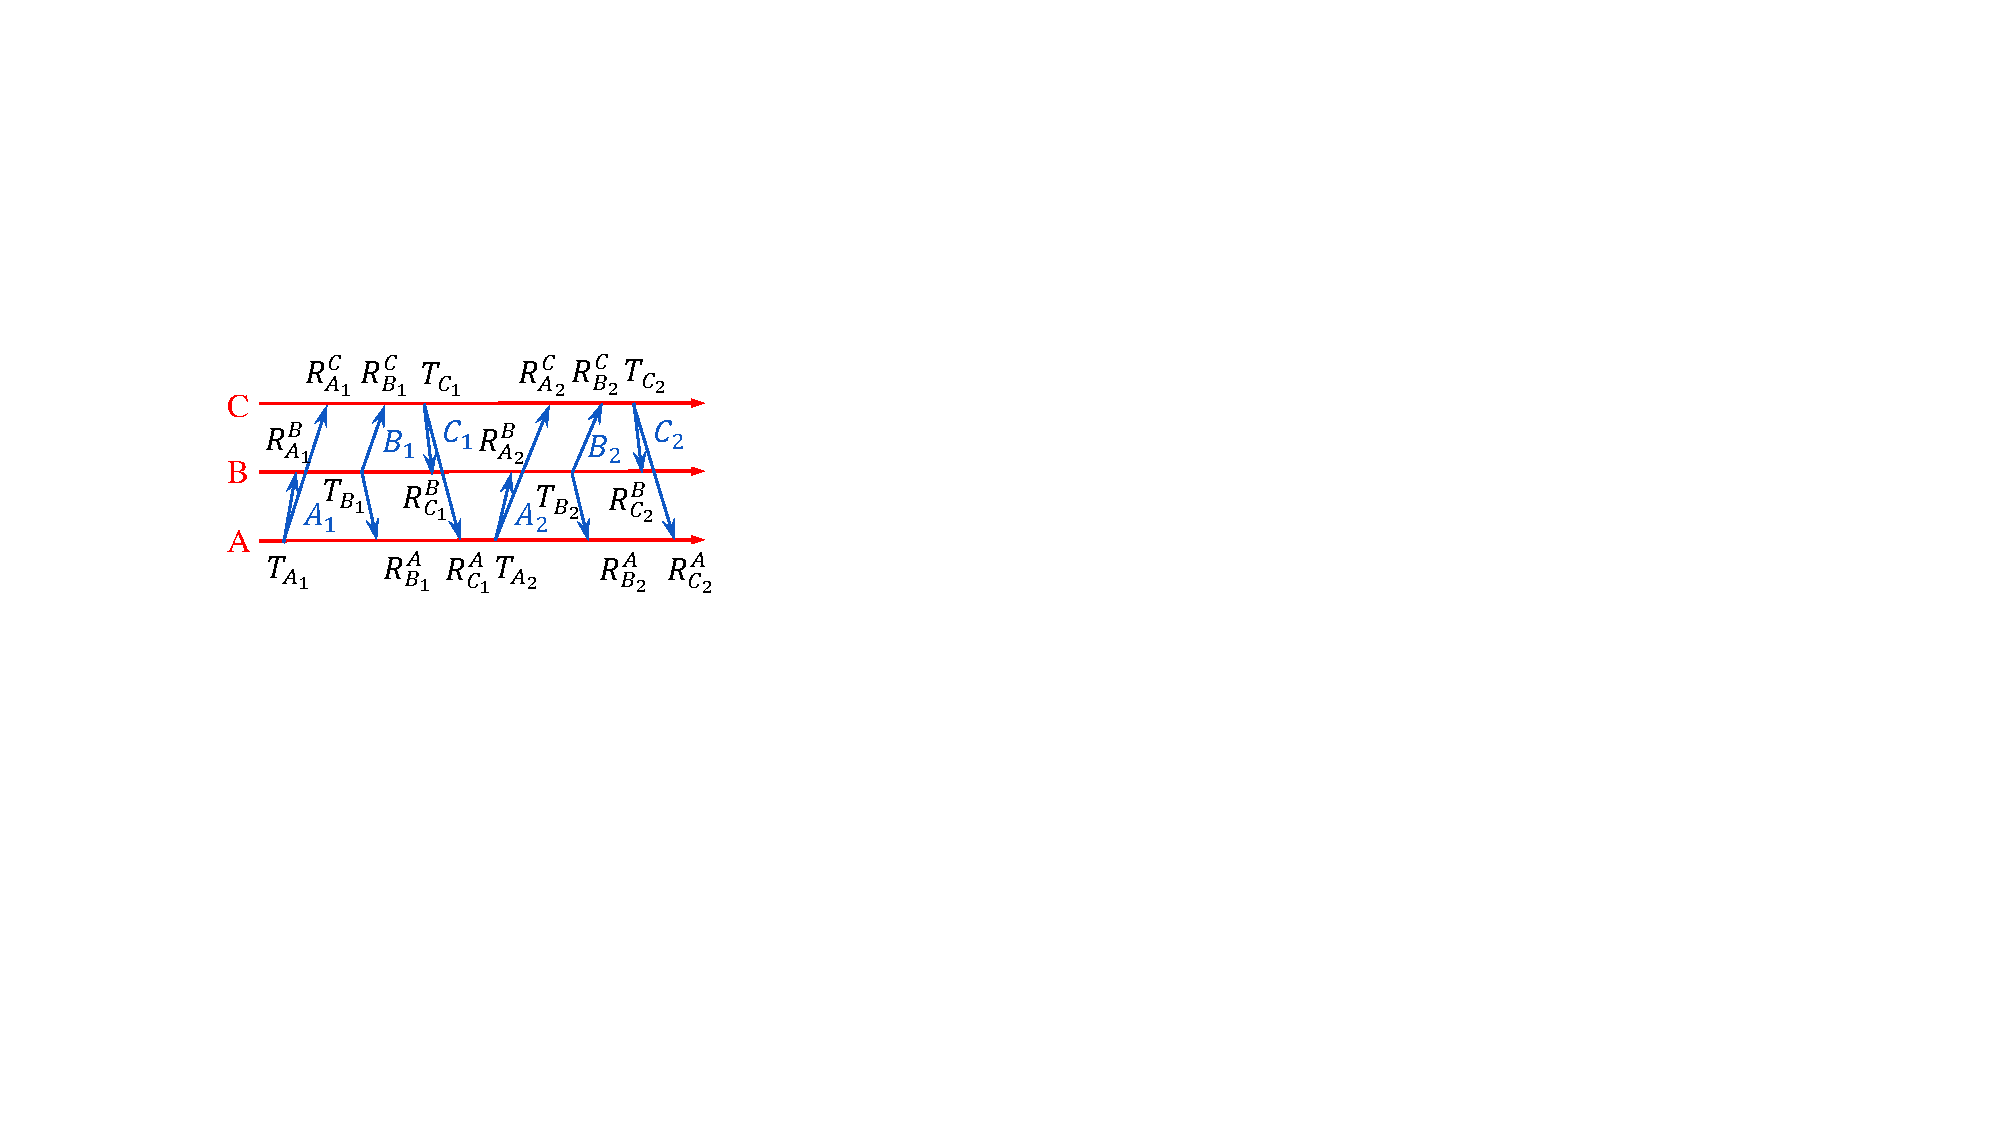
\includegraphics[width=.38\textwidth]{figures/content/chapter3/toyexample1.pdf}
  }
  \quad\quad
  \subfloat[收集足够的时间戳来计算飞行时间\label{fig:3_1b}]{
    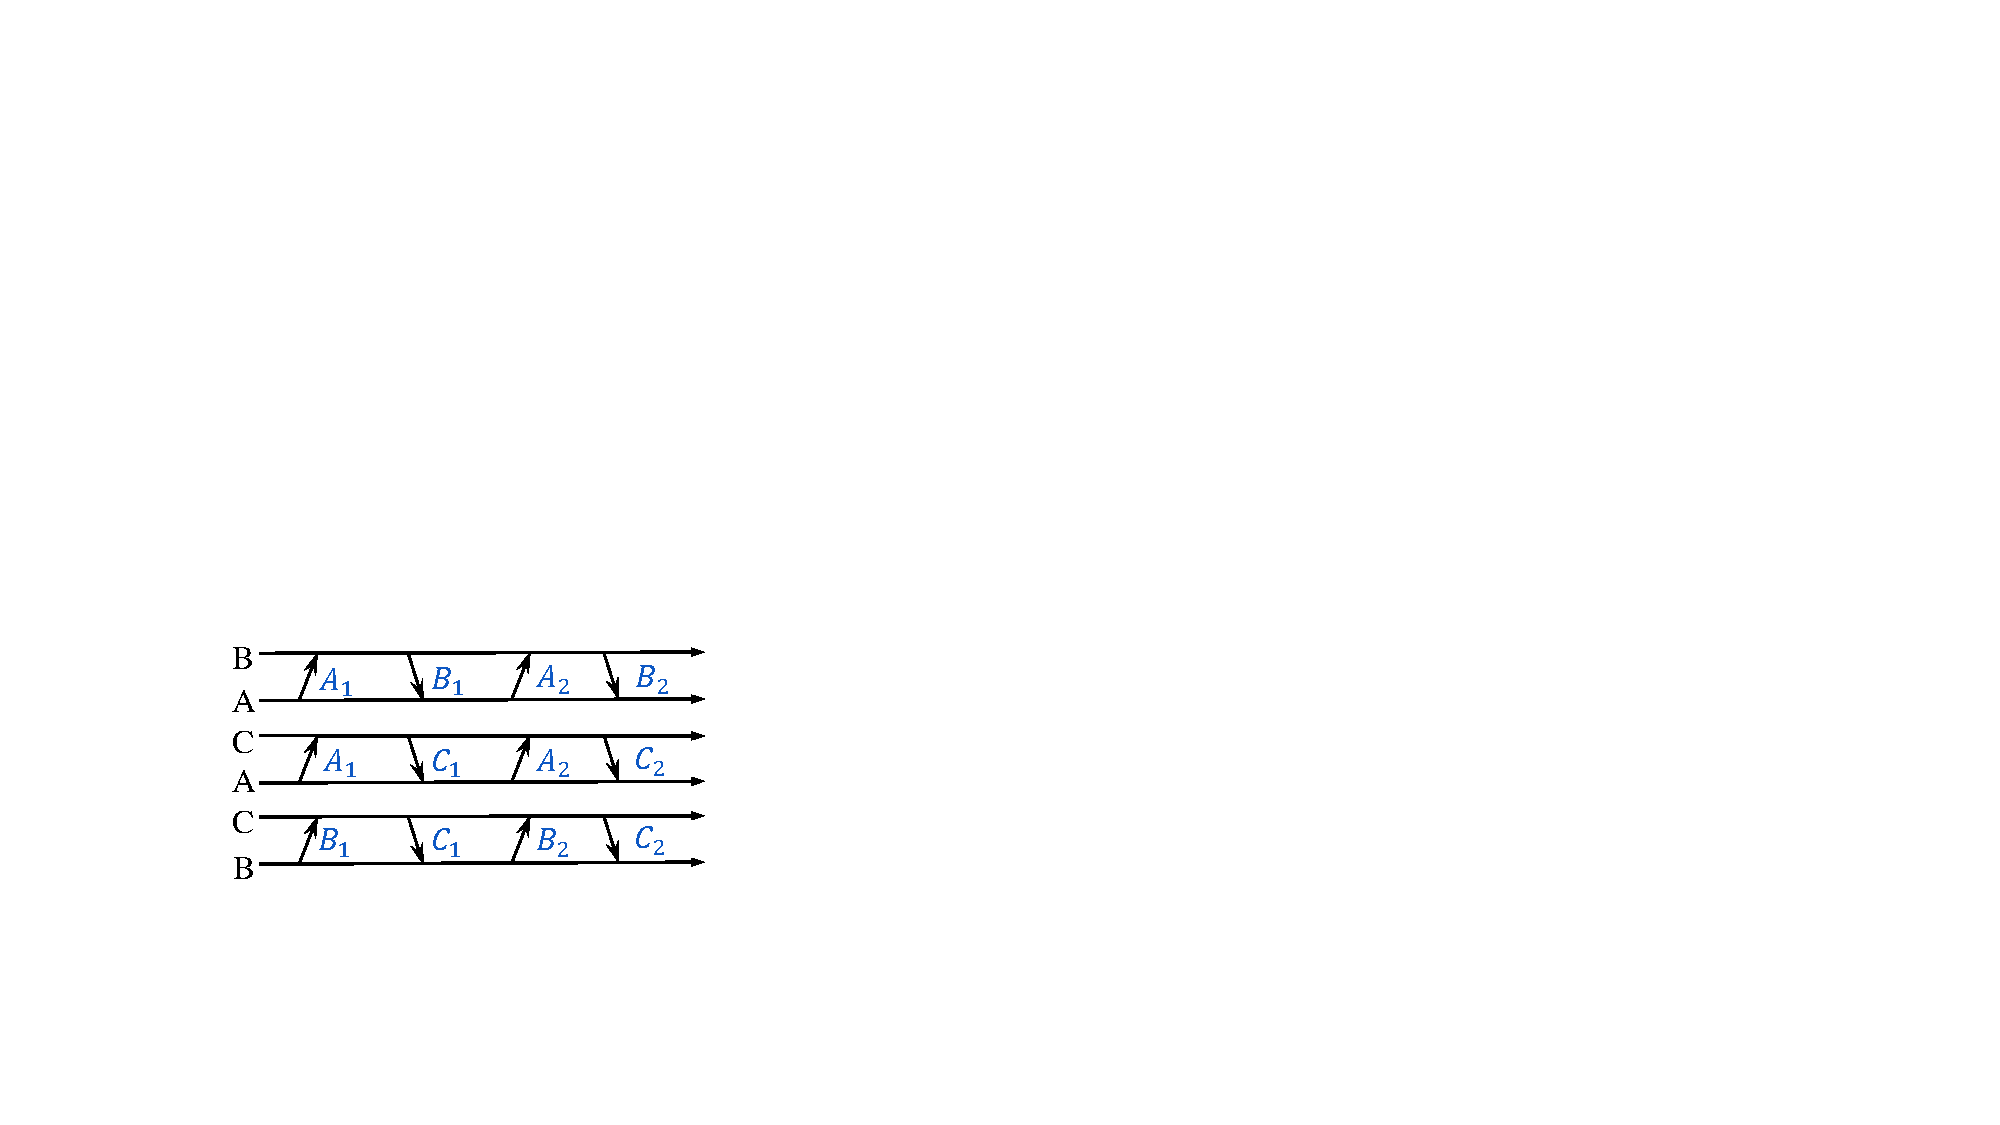
\includegraphics[width=.38\textwidth]{figures/content/chapter3/toyexample2.pdf}
  }
  \caption{无人机集群场景的集群测距协议示意图}
  \label{fig:3_1}
\end{figure}

每个测距报文包含报文标识信息（包括发送无人机的标号及报文序列号）、该无人机最近一次测距报文的发送时间戳，以及从所有邻居无人机节点收集到的接收时间戳。
为了支持相对定位，测距报文必须携带发送方无人机的速度、偏航率和高度信息，以便邻居可以利用这些信息进行相对定位估计。
因此，测距报文的数据字段如图\ref{fig:3_insert}所示。

\begin{figure}[htbp]
  \centering
  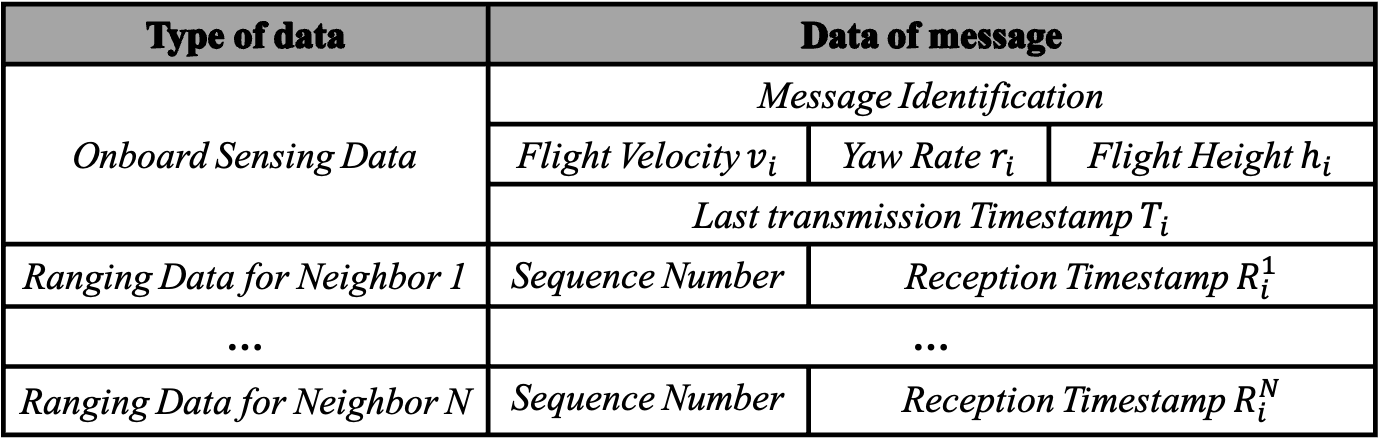
\includegraphics[width=.8\linewidth]{figures/content/chapter3/dataofmessage.png}
  \caption{测距报文中所包含的相对定位相关的数据}
  \label{fig:3_insert}
  \end{figure}


根据飞行时间的计算原理\cite{9179124}，完成一次飞行时间估计需要六个时间戳（$T_p$, $R_p$, $T_r$, $R_r$, $T_f$, $R_f$）。
因此，在该测距协议中，每一个无人机都有一个专用的数据结构，用于存储与其相关的时间戳信息，该数据结构称为测距表。
假设无人机 $A$ 需要与多个邻居无人机进行测距，记$Y$为其中任意一个邻居无人机。
无人机 $A$ 与 $Y$ 之间的报文交互过程如图 \ref{fig:3_2}(a) 所示。
图 \ref{fig:3_2}(b) 展示了无人机 $A$ 在接收到来自无人机 $Y$的第二条测距报文$Y_{2}$时，其测距表中已存储的时间戳信息。
此时，测距表中已包含满足飞行时间计算条件的六个时间戳，从而可以完成无人机$A$ 与无人机 $Y$ 之间的飞行时间估计。

\begin{figure}[htbp]
  \centering
  \subfloat[带有时间戳的报文交换\label{fig:3_2a}]{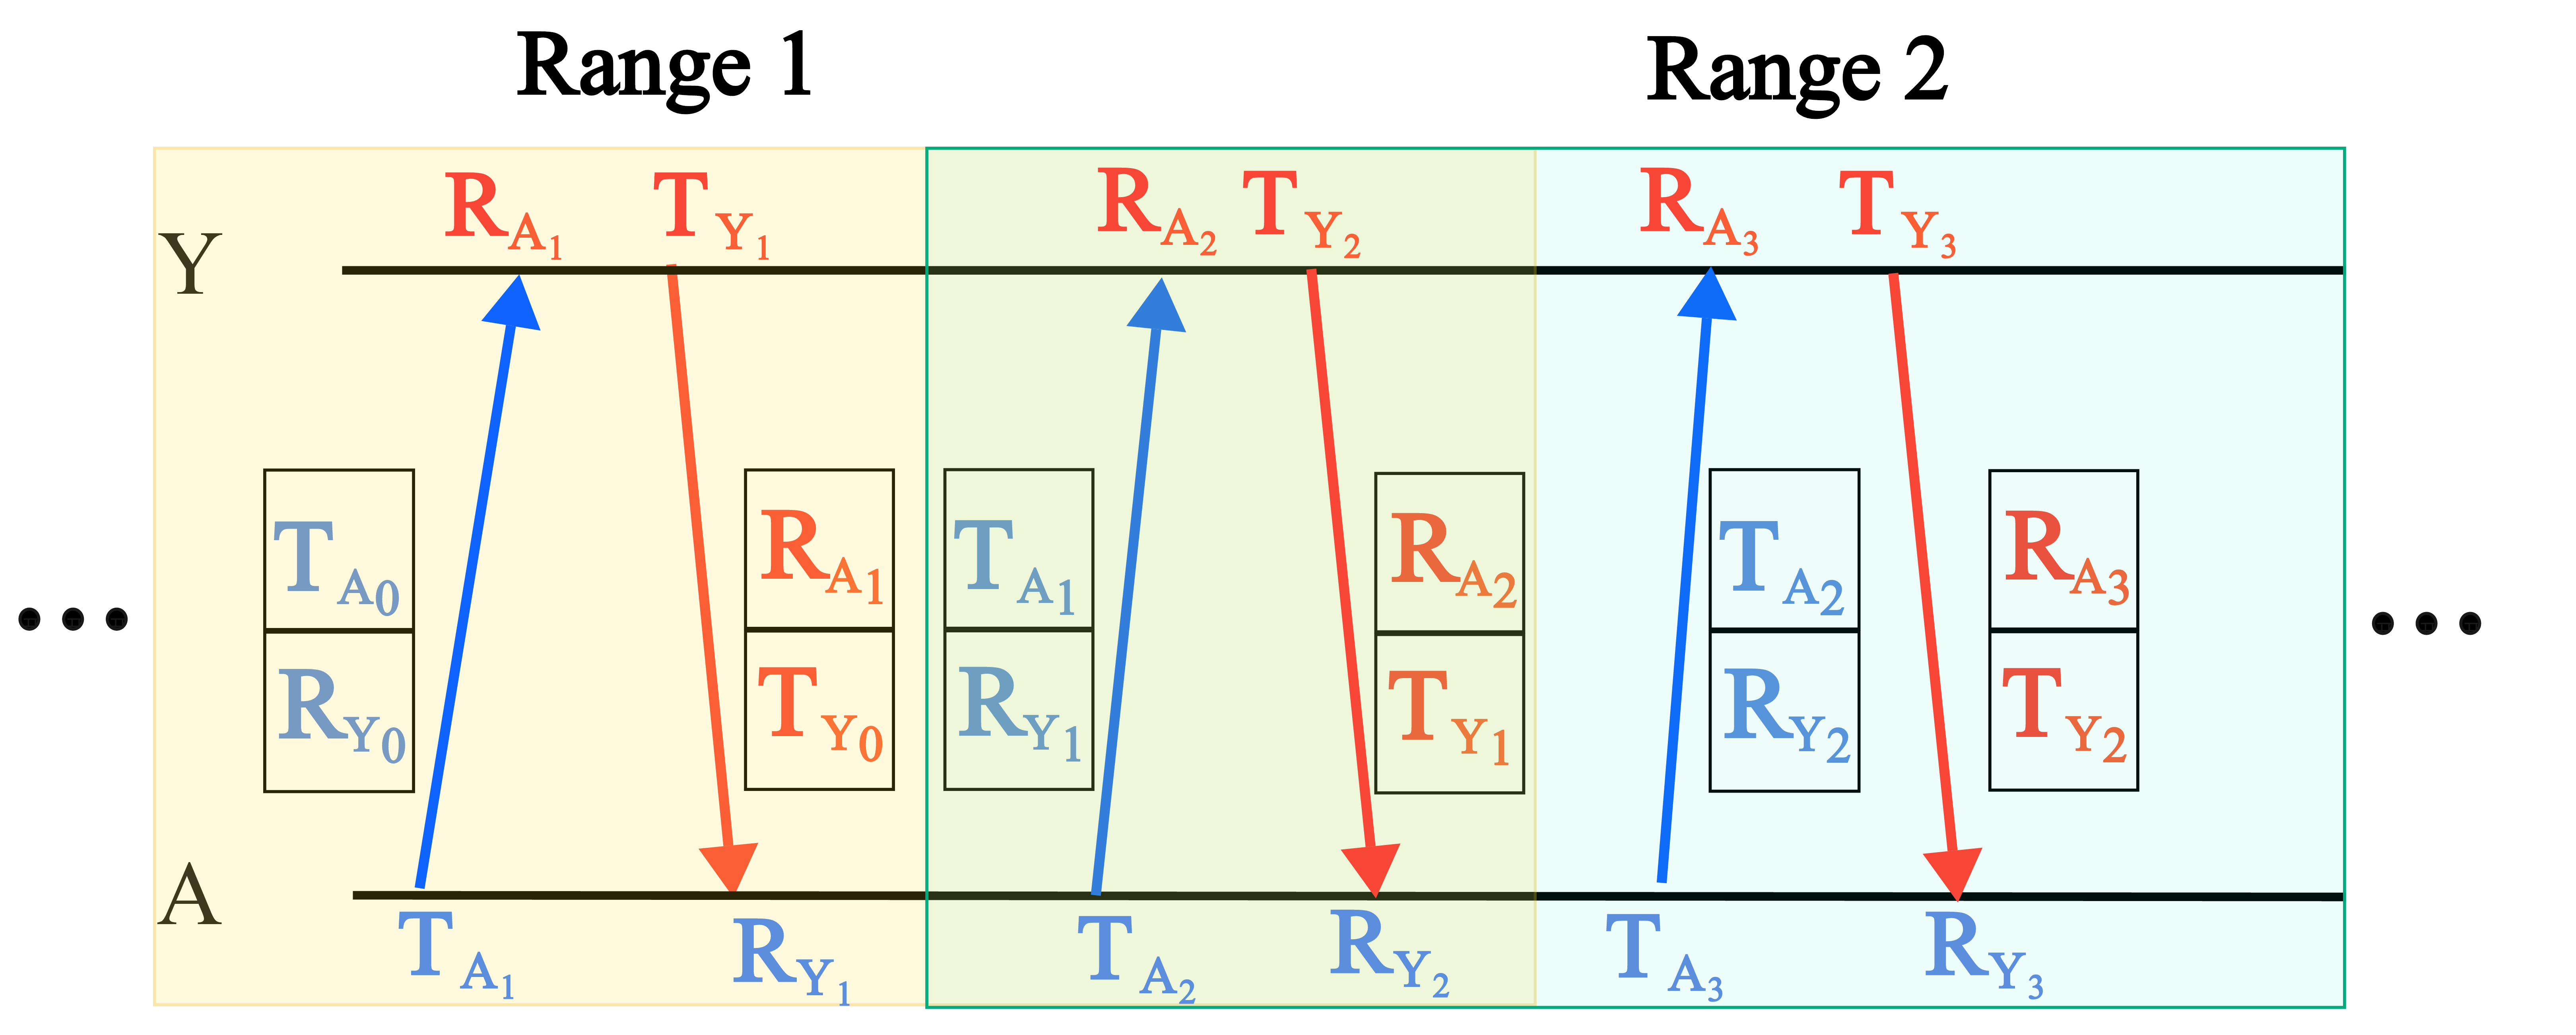
\includegraphics[width=.45\textwidth]{figures/content/chapter3/mes_ex_A_Y.png}}
  \quad\quad
  \subfloat[计算距离的集群测距表\label{fig:3_2b}]{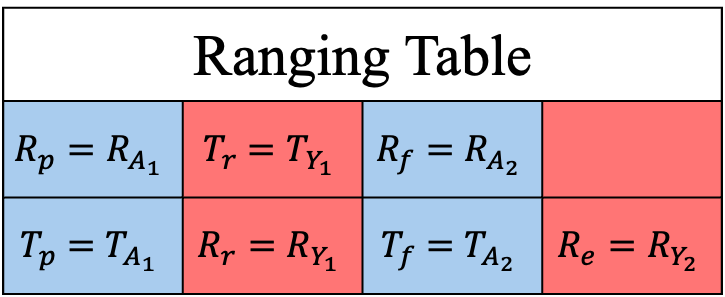
\includegraphics[width=.38\textwidth]{figures/content/chapter3/rangingTable.png}}
  \caption{无人机集群中的报文交换与测距表}
  \label{fig:3_2}
  \end{figure}



在大规模集群测距场景中，众多无人机同时参与集群测距。
各无人机需频繁处理测距报文，包括从邻居无人机接收报文（RX）以及向邻居无人机发送报文（TX），使系统长期处于高通信负载状态。
如图 \ref{fig:3_3} 所示，在理想情况下，无人机报文的发送与接收均按照预设周期进行，两次发送报文时间的间隔具有严格的确定性。
然而在实际应用中，由于硬件芯片普遍存在时钟偏\cite{zhao2022clockids}问题，即使在集群测距协议中为各无人机配置了相同的测距周期，
其本地时钟仍难以实现精确同步，进而导致不同无人机连续两次发送报文的时间戳差值不一致。
如图 \ref{fig:3_4} 所示，不同无人机的时钟存在细微差异，导致 无人机两次发送报文的时间戳随时间逐渐偏移并接近。
最终，两个无人机不可避免地会在非常相近的时间发送报文，从而导致产生长时间的连续测距失败现象。
例如 图\ref{fig:3_4} 中展示的$Y_{2}$，$Y_{3}$报文导致的测距失败。

  \begin{figure}[htbp]
    \centering
    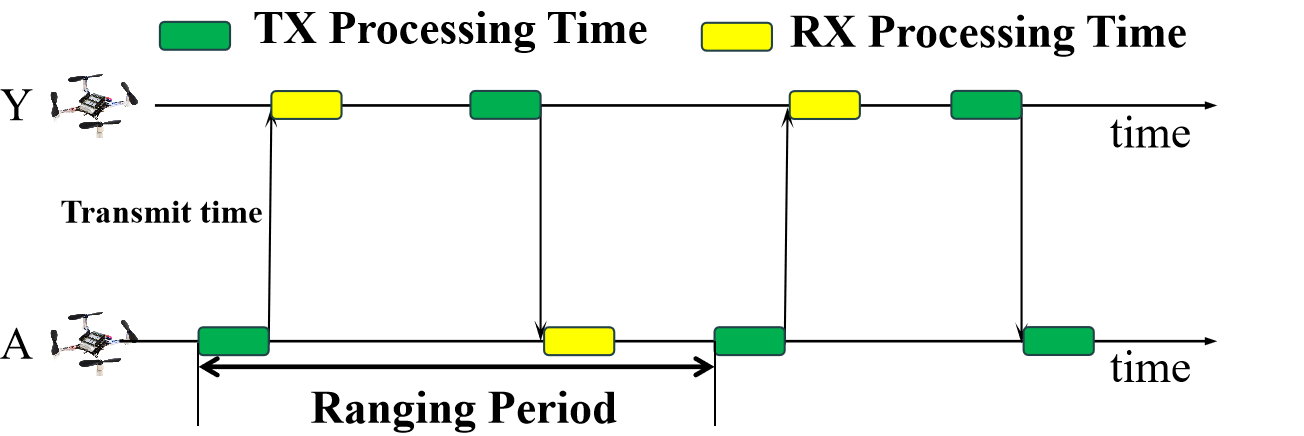
\includegraphics[width=.6\linewidth]{figures/content/chapter3/TxRxProcessTime.png}
    \caption{理想情况下的集群测距}
    \label{fig:3_3}
    \end{figure}

此外，如图 \ref{fig:3_4} 所示，测距报文在网络传输过程中可能发生乱序到达。
例如，来自无人机$Y$的第 7 条测距报文$Y_{7}$可能先于其关联报文到达。
在此情况下，无人机$Y$发送的测距报文无法与无人机$A$发送的关联报文正确匹配，
导致计算飞行时间所需的关键时间戳信息不完整，使得无人机$A$在接收到该报文后无法完成有效测距。
该测距失败的根本原因在于测距报文匹配失败所引起的时间戳缺失问题。
上述问题在无人机密度较高、通信负载较大的大规模集群测距场景中尤为显著，严重制约了系统的测距成功率与整体性能。



\begin{figure}[htbp]
  \centering
  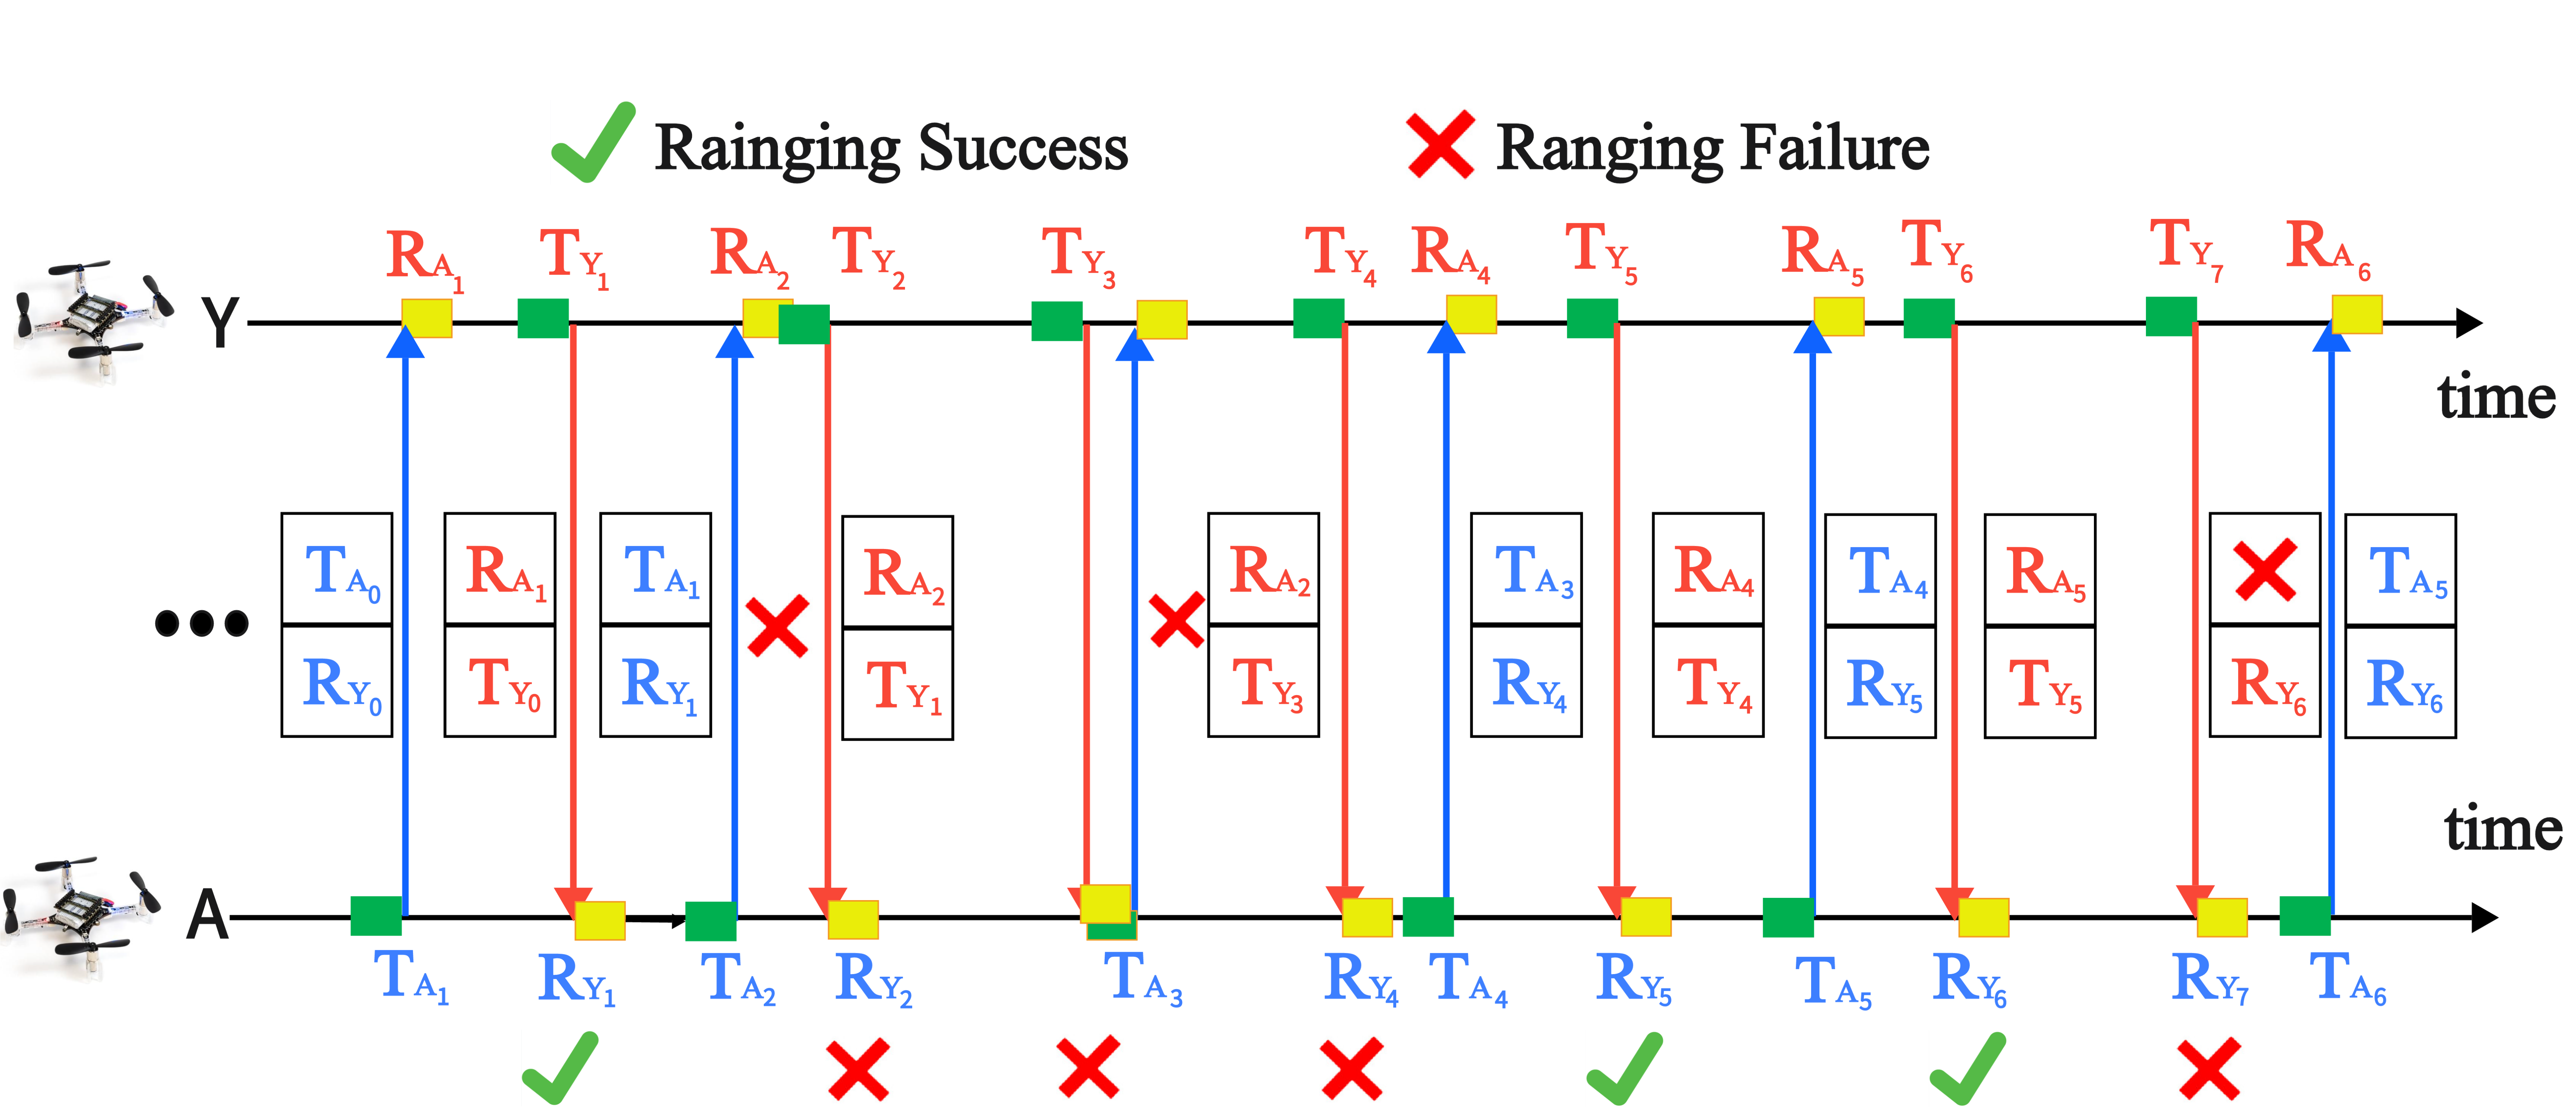
\includegraphics[width=.8\linewidth]{figures/content/chapter3/clockSkew.png}
  \caption{由于时钟偏移所导致的测距失败}
  \label{fig:3_4}
  \end{figure}


因此，我们的研究动机源于三个方面:首先，当我们尝试将此前提出的集群测距协议直接应用于相对定位任务时，会面临着一个难以回避的两难抉择：
一方面，采用静态固定的测距周期，在大规模集群中会不可避免地产生持续的测距报文冲突；
另一方面，引入动态随机的测距周期虽然能够在一定程度上缓解测距冲突，但却会增加测距报文之间无法正确匹配的概率，从而引入新的测距失败问题。
其次，一旦测距报文的交互发生不匹配，部分关键时间戳信息将不可避免地丢失，使得原始集群测距协议无法完成距离计算。
然而，我们注意到，即使时间戳不完整，测距报文中仍可能保留部分有效时间戳信息。
这引出了一个关键问题：在收到报文中存在时间戳缺失的情况下，是否仍可利用现有时间戳信息实现距离估计?
该问题在相对定位应用中尤为关键，也直接促使我们思考设计一种更适用于大规模集群相对定位的新型测距协议。
此外，在通过引入随机性以缓解测距失败时，随机参数的合理选取及其对系统性能的影响仍缺乏系统性的分析与评估方法。
这使得现有测距协议在大规模集群中的性能表现难以预测，也限制了进一步优化的空间。

根据上述内容的分析，测距失败主要由两类原因引起：报文丢失和测距报文不匹配。
对于报文丢失的情况，如图 \ref{fig:3_4} 所示，当无人机 $A$ 在发送自身测距报文时无法接收到无人机 $Y$ 测距报文, 因此无人机$Y$发送的测距报文丢失（如 $Y_{2}$ 和 $Y_{3}$，最终无法计算距离，导致测距失败。

另一方面，在测距报文不匹配的情形下，即便无人机$A$ 成功接收到来自无人机 $Y$ 的测距报文，
该报文中也缺少用于计算飞行时间的关键时间戳（即 无人机$A$报文 的接收时间戳）。
以图 \ref{fig:3_4} 中的报文$Y_{7}$ 为例，由于节点 $Y$ 在发送 $Y_{7}$ 之后才接收到来自 $A$ 的报文 $A_{6}$，导致 $Y_{7}$ 中未包含对应的接收时间戳，从而无法完成飞行时间计算，测距最终失败。

由于硬件时钟偏移通常远小于通信与处理延迟，这类问题往往会导致无人机在一段较长的时间内连续的测距失败。
此外，测距报文混乱交换进一步加剧了报文不匹配现象，显著提高了测距失败的发生概率。

上述分析均已通过实验结果得到验证。
在一组实验中，保持一个无人机静止，另一个无人机以 1 m/s 的速度往返运动，采用原始集群测距协议并将测距周期设置为 $60$ ms。
实验结果如图\ref{fig:3_4} 所示，可以观察到测距过程中周期性地出现连续测距失败的现象，在该实验配置下，每次连续测距失败的持续约 $0.4$ s。

\begin{figure}[htbp]
  \centering
  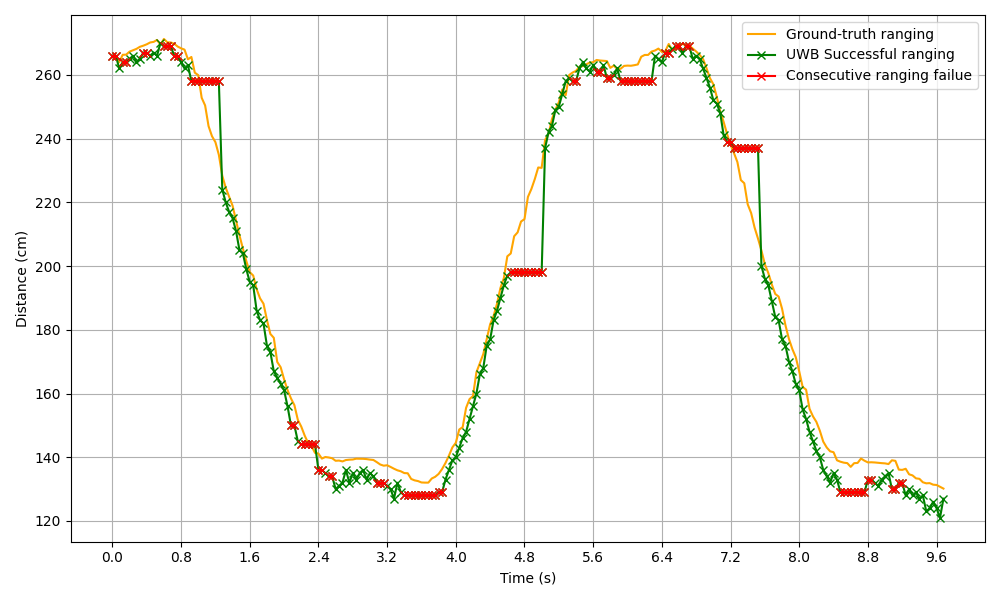
\includegraphics[width=.6\linewidth]{figures/content/chapter3/consecutive_rangingfailuresv2.png}
  \caption{静态的固定测距周期所导致的连续测距失败现象}
  \label{fig:3_5}
  \end{figure}

在另一组实验中，测距周期在 $0–60 $ms 之间随机生成。
实验结果如图 \ref{fig:3_5} 所示，测距失败次数显著增加，从 $9.6$ s 内的 $118$ 次上升至 $9.7$ s 内的 $204$ 次,这些测距失败都是由于测距报文不匹配的原因产生的。

当无人机集群处于高动态、高密集场景时，连续测距失败和测距报文不匹配现象不仅降低了测距可靠性，还会引发额外的通信开销和系统负担。
然而值得注意的是，尽管报文$Y_{7}$ 无法直接用于原始集群测距协议中的距离计算，其仍保留了前一轮测距过程中的发送时间戳。
这一现象进一步启发我们思考：是否可以利用这些残留时间戳信息，实现额外的距离估计？


\begin{figure}[htbp]
  \centering
  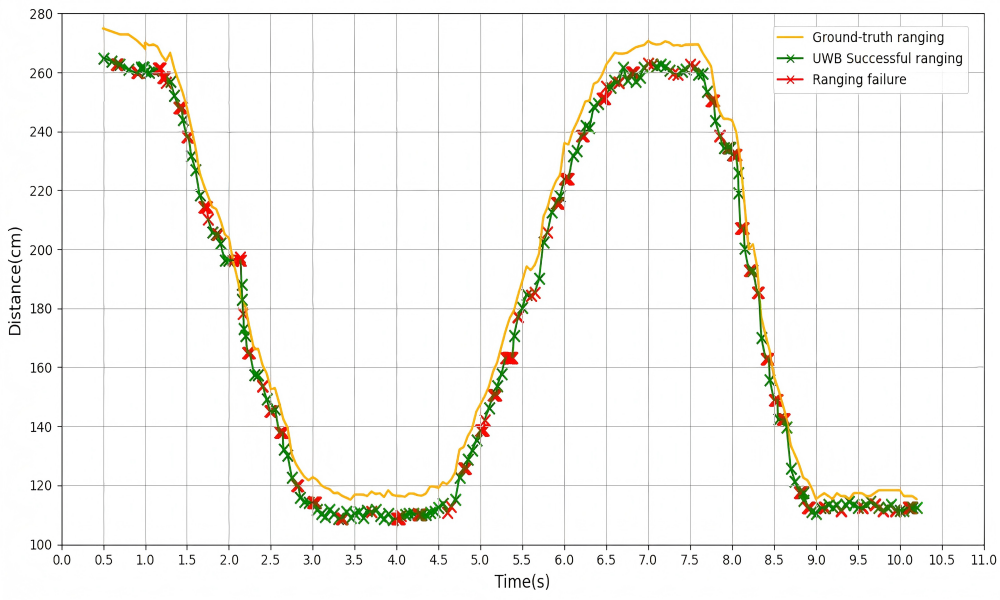
\includegraphics[width=.6\linewidth]{figures/content/chapter3/experiment_w_large.png}
  \caption{测距报文不匹配而导致的测距失败次数增多现象}
  \label{fig:3_6}
  \end{figure}
基于上述分析与实验观察，本文旨在设计一种面向大规模相对定位应用的新型测距协议，以提升在高动态、高密集场景下的测距成功率与系统鲁棒性。
同时，如何系统性地评估该协议在大规模集群中的性能表现，也是本文需要重点关注的问题之一。

下面的小节本文提出并系统分析了一种面向相对定位的鲁棒超宽带测距协议。
该协议首先通过在测距周期中引入随机抖动参数，对测距周期进行随机化，以有效缓解连续测距失败的问题。
然而，抖动的引入也可能带来报文交换不匹配概率增大的风险：当抖动幅度过大时，某一无人机可能在邻居无人机发送下一条测距报文之前连续发送多条报文，
导致这些报文缺乏完整的时间戳信息，使对方无人机无法完成距离计算，最终引发测距失败。
因此，降低报文不匹配发生的概率对于协议的可靠运行至关重要。

针对由报文不匹配导致的时间戳缺失问题，本文进一步提出了一种权衡式测距方法，在鲁棒性与测距成功率之间取得有效平衡。
最后，鲁棒集群测距协议给出了一种高效机制，用于在动态密集集群场景下实现最优性能所需的抖动参数取值，从而提升整体测距稳定性与系统性能。
\subsection{基于扰动的理论分析}
本节首先对由报文冲突导致的连续测距失败次数进行了分析。
直观来看，引入随机化的测距周期似乎可以缓解连续测距失败的问题。
然而，分析结果表明，单纯地增加周期抖动并不能有效降低测距失败的发生频率，因此也无法从根本上减少由报文冲突引起的测距失败。

\begin{definition}[抖动]
测距周期$P$通过引入随机抖动进行随机化处理，其形式为 $P = p + w$。其中，基数 $p$ 为固定值并且$p < P$。
随机变量 $w$ 服从离散均匀分布，其取值范围为 $\left\{0,1,…,W \right\}$，概率质量函数为：
$P(w=k)=\frac{1}{W+1}$。
参数$W$ 被称为随机窗口大小或抖动。因此 ，测距周期的期望值$\overline{P} = E(p + w) = p + W/2$。

\end{definition}

\begin{theorem}
由报文冲突引起的测距失败的平均频率为$\left\lfloor \frac{2L}{\overline{P}^{2}}\right\rfloor$，
其中$L$ 表示 TX 的处理时间。值得注意的是，测距失败的频率与引入的抖动幅度无关。
\end{theorem}

换言之，只要测距周期的期望保持为$P=\overline{P}$ ，是否引入抖动并不会影响由报文冲突导致的测距失败次数。
为证明定理 1，下面首先给出并证明若干引理。

\begin{lemma}
\label{lemma:nojitter}
当不存在抖动（即$W=0$）时，无人机之间可能出现连续的测距失败。
此时，由报文冲突引起的测距失败频率可表示为$f=\left\lfloor \frac{2L}{P^{2}}\right\rfloor$。
    \end{lemma}

证明：考虑两个无人机 $A$和$Y$正在进行集群测距的场景，并且二者采用相同的测距周期 $P$毫秒。
无人机$A$ 和 $Y$ 的单位毫秒时钟偏移率分别记为 $e_A$ ​ 和$e_Y$。
因此，在每个测距周期内，两个无人机累积的时钟偏移分别为 $Pe_A$  ​ 和 $Pe_Y$ 。 
不失一般性，假设 $e_A > e_Y$ ​ 。
则在一个测距周期内，两个无人机之间的报文发送时间差将产生 $P(e_A - e_Y)$ 的漂移。 

当两个无人机之间的报文发送时间差的绝对值小于 $L$  时，其中一个无人机将发生报文冲突并导致报文丢失，从而引发一次测距失败。
由于时钟偏移的存在，这种冲突状态将不可避免地周期性出现。 
我们将连续发生测距失败的时间周期定义为 $P_c=\frac{P}{e_{A}-e_{Y}}$ 。
在一个周期内，测距失败的次数可表示为 $k=\left\lfloor \frac{2L}{P(e_{A}-e_{Y})}\right\rfloor$​ , 而对应的持续时间为 $P_{s}=\frac{2L}{(e_{A}-e_{Y})}$。 
因此，由报文冲突引起的测距失败频率 $ f$ 可计算为$f=\frac{k}{P_{c}}=\left\lfloor \frac{2L}{P^{2}}\right\rfloor$。​\qed

\begin{lemma}
在引入抖动 $W$ 的情况下，由报文冲突引起的测距失败频率仍可表示为$f=\left\lfloor \frac{2L}{\overline{P}^{2}}\right\rfloor$。
  \end{lemma}
证明：
当无人机$A$ 与 $ Y$ 的通信持续时间足够长时，在时钟偏移的影响下，两者的报文发送时间之间必然存在一个时间差 $\Delta t$，其中$\Delta t = TX_{A}-TX_{Y}$。
该时间差  $\Delta t$ 在区间 $[0, P]$ 上服从均匀分布，即 $\Delta t \in U(0, P)$。
 当 $ \left| \Delta t \right | < L $ 时，将发生报文冲突，从而导致测距失败。
 因此，单次测距发生失败的概率为 $\frac{2L}{P}$​ 。 
在引入周期随机化（抖动）后，测距失败的平均发生频率可表示为 $f^{w}=\lfloor \frac{2L}{P^{2}}\rfloor$。
​\qed

由上述分析可知，只要测距周期的期望满足$P=\overline{P}$，则有$f=f^{w}$​，
即无论是否引入抖动，测距失败的总体发生频率保持不变。
这表明，对测距周期设置抖动并不会影响由报文丢失引起的测距失败频率。
换言之，由报文冲突导致的测距失败是不可避免的。

既然由报文冲突引起的测距失败不可避免，那么一个更为关键的问题是：抖动幅度的选择将如何影响 鲁棒集群测距协议在相对定位中的鲁棒性？

以下定理刻画了抖动参数选取过程中所面临的权衡与困境。

\begin{theorem}
连续测距失败平均次数的上确界可计算为 
\begin{equation}
  \sup K_{avg}=1+\frac{2}{W+1}+\frac{1}{W^2+W}, 
\end{equation}
而测距报文不匹配发生的概率可计算为
\begin{equation}
  P(C)=\frac{1}{6P}\frac{W(W^2+3W+2)}{(W+1)^2}.
  \end{equation}
由此可以看出，随着抖动参数 $W$ 的增大，连续测距失败的平均次数虽然有所降低，但测距报文不匹配的概率却随之增加，从而导致整体测距失败次数反而增多。
\end{theorem}

证明：定义事件 $Y_{i}$ ​ 表示发生连续的$i$次测距失败。 
在两个无人机通信测距过程中，精确计算测距失败的概率十分复杂。
为简化分析，本文转而计算连续测距失败平均次数的上确界。
因此，下文给出的概率值均为其上确界。
我们的研究重点在于连续测距失败现象，具体而言，是在发生一次测距失败之后，是否会继续接连不断的发生测距失败。
在该情形下，可以将首次测距失败的发生概率视为 $1$，即 $P(Y_{1})=1$。

当两个无人机进入连续测距失败阶段时，只要它们连续两次发送报文的时间差大于该连续失败阶段的持续时间，则下一次报文丢失将不会发生。
设连续测距失败阶段的持续时间为  $L$ ms。
基于上述分析，在连续测距失败阶段内，两个无人机的测距周期需满足 $\left | P_{A}+P_{A}e_{A}-P_{Y}-P_{Y}e_{Y}\right|>L$,
其中，$P_{A}$ 和$P_{Y}$分别表示无人机$A $和 无人机$Y$ 的测距周期。
在满足上述条件的情况下，将不会发生测距失败。

在实验章节中的实验结果表明，连续测距失败阶段的持续时间满足 $L<1 \text{ms}$。
此外，在单个测距周期内，两个无人机之间的时钟偏移差远小于 $1$ ms。
那么只要下一次测距时引入的抖动满足$w_{A}-w_{Y} \ne 0$，抖动就可以使系统离开连续测距失败阶段。

接下来，我们将分析上述情形发生的概率。
定义 $\Delta w = w_{A}-w_{Y}$, 并记 $\Delta w $ 的概率为 $P(\Delta w)$。
其中， $\Delta w $ 服从表 \ref{tab:Probabilityofdeltaw} 所示的概率分布。

\begin{table}[htbp]
  \centering
  \caption{$\Delta w$ 的概率分布}
  \label{tab:Probabilityofdeltaw}
  \begin{tabular}{|c|c|c|c|c|c|c|c|}
    \hline
    $\Delta w$ 
    & $-W$ 
    & $-W+1$ 
    & $\cdots$ 
    & $0$ 
    & $\cdots$ 
    & $W-1$ 
    & $W$ \\
    \hline
    $P(\Delta w)$ 
    & $\frac{1}{(W+1)^2}$ 
    & $\frac{2}{(W+1)^2}$ 
    & $\cdots$ 
    & $\frac{W+1}{(W+1)^2}$ 
    & $\cdots$ 
    & $\frac{2}{(W+1)^2}$ 
    & $\frac{1}{(W+1)^2}$ \\
    \hline
  \end{tabular}
\end{table}

在无人机进入连续测距失败阶段后，单次继续发生测距失败的概率为 $\frac{1}{W+1}$​ 。
 当$i >1$时， $W$ 取连续  $i$次为 $0$，而第 $i+1$ 次取值不为 $0$，这意味着发生了连续 $i$ 次测距失败。
 因此，连续发生 $i$ 次测距失败的概率  $P(B_{i})$ 可表示为 $\frac{W}{(W+1)^{i}}$。
 由此，可以计算连续测距失败次数平均值的上极限为：

\begin{equation}
\begin{aligned}
\sup K_{avg}&= \lim_{i \to \infty} \sup E(k)=\sum_{i=1}^{\infty} iP(Y_{i})\\
&=1+2\frac{W}{(W+1)^2}+3\frac{W}{(W+1)^3}+...+i\frac{W}{(W+1)^{i}}\\
&=1+\frac{2}{W+1}+\frac{1}{W^2+W}\\
\end{aligned}
\end{equation}

在对测距周期进行随机化之后，连续测距失败的概率将随着 $W$ 的增大而逐渐降低。
与此同时，连续测距失败问题也将得到显著缓解。

接下来，为了尽量减少测距报文不匹配的发生，我们对测距报文不匹配的概率进行分析。
我们考虑在足够长时间的通信测距过程的条件下，计算两个无人机发生测距报文不匹配的概率。
定义事件 $C$ 为两无人机之间发生了一次测距报文不匹配。
显然，当 $W$ 取值过大时，事件 $ C$ 的发生概率将显著升高，这不是我们所期望的。
因此，需要对 $ W$ 的取值范围加以限制，以尽可能降低事件 $C$ 的发生概率。
如图 \ref{fig:3_7}展示了一种特殊情形。
在该情形下，无人机 $A$ 发送了一次测距报文，而无人机 $Y$ 恰好发送了两次测距报文。
其中，无人机 $Y$ 的测距周期在连续两次中均取最小值 $P-\frac{W}{2}$ ，而无人机 $A$ 的测距周期取最大值 $P+\frac{W}{2}$。
只要$W$ 的取值范围满足 $2(P-\frac{W}{2})>P+\frac{W}{2}$, 即 $W<\frac{2P}{3}$​ ,
即可保证在两个无人机同时发送测距报文之后，事件 $ C$ 不可能会发生。 
 \begin{figure}[htbp]
  \centering
  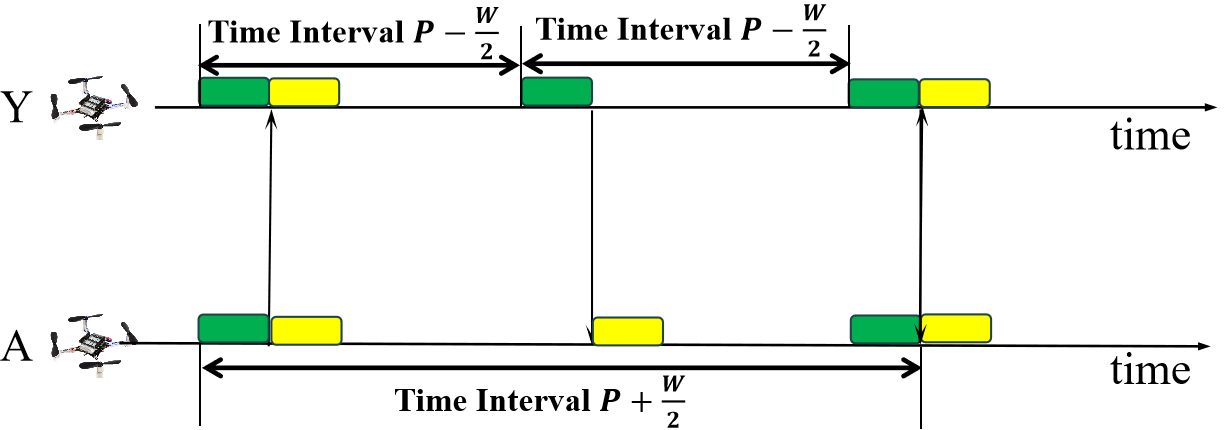
\includegraphics[width=.7\linewidth]{figures/content/chapter3/ProcessTime.png}
  \caption{限制抖动大小的特殊情况}
  \label{fig:3_7}
  \end{figure}
  
当无人机$ A$ 先发送测距报文、随后无人机$Y$ 发送测距报文时，两无人机能够完成一次正常测距。
若在此之后，无人机 $A$ 在无人机$ Y$ 已发送测距报文的情况下再次发送报文，则会发生测距报文不匹配现象。
因此，当条件 $p+w_{A}>p+w_{Y}+\Delta t$成立时，将发生测距报文不匹配。
事件 $ C$ 的发生等价于 $\Delta w>\Delta t$。 
为计算概率 $P(\Delta w> \Delta t)$，首先需要将 $\Delta t$ 的取值范围划分为若干较小的区间，并分别讨论在不同区间内满足条件的 $\Delta t$ 取值范围。
由于必须满足 $\Delta w > \Delta t$，能够满足该条件的 $\Delta t$ 的最大取值为 $W$。
因此，$\Delta t$的取值区间可划分为$\left [ 0,1\right ),\left [ 1,2\right),...,\left[ W-1,W\right)$。
当$\Delta t \in \left [ 0,1\right )$ 时，满足条件的 $\Delta w$取值为 $1,2,...,W$。
同理，当  $\Delta t$ 落入其他区间时，也可以得到相应满足条件的$\Delta w$ 取值范围。
综合上述分析，可最终推导得到事件 $C$ 的发生概率如下所示：
 \begin{equation}
  \begin{aligned}
  P(C)=&\frac{1}{P}\frac{(W+1)W}{2(W+1)^2}+\frac{1}{P}\frac{W(W-1)}{2(W+1)^2}+...+\frac{1}{P}\frac{2}{2(W+1)^2}\\
  =&\frac{1}{2P(W+1)^2}\sum_{k=0}^{W-1}(W+1-k)(W-k) \\
  =&\frac{1}{6P}\frac{W(W^2+3W+2)}{(W+1)^2}
  \end{aligned}
  \end{equation}
因此，我们得到了在对测距周期进行随机化之后，测距不匹配发生的概率。
​\qed

\subsection{权衡测距机制的设计}

尽管通过在测距周期中引入随机性可以显著减少连续测距失败的次数，但该方法也引入了一个新的问题：由于时间戳缺失而导致的测距失败。
当抖动设置过大时，测距周期的波动幅度显著增加，从而更容易引发测距报文不匹配的现象。

如图 \ref{fig:3_8} 所示，当两次测距报文连续发送而且在发送间隔中未接收到来自相邻无人机对应报文的情况下，就会发生消报文不匹配现象。
此时，这些已发送的测距报文缺少测距协议所需的接收时间戳，导致测距过程无法正常完成。
例如，当无人机$A$ 接收到不包含接收时间戳的 $Y_{3}$报文时，与之对应的 $A_{3}$ ​报文的发送时间戳和接收时间戳均未记录在测距表中，从而无法计算最新的测距结果。

\begin{figure}[htbp]
  \centering
  \includegraphics[width=.7\linewidth]{figures/content/chapter3/Problemwithjitter.png}
  \caption{报文不匹配现象}
  \label{fig:3_8}
  \end{figure}

由于时间戳缺失而引起的测距失败，会导致连续测距失败更加频繁且持续时间更长。
该问题源于测距周期的随机化，因此在一定程度上是不可避免的。
所幸的是，我们发现可以通过利用历史时间戳信息来有效缓解这一问题。
在鲁棒集群测距协议中，提出了一种权衡测距方法，用于解决由时间戳缺失导致的测距失败问题。
为此，我们设计了一种新的测距表结构，如图 \ref{fig:3_9} 所示，用以支持权衡测距机制。
在该方法中，当接收到缺失时间戳的测距报文时，系统会调用并使用历史报文中已存储的时间戳来参与距离计算，从而避免测距的失败并降低连续测距失败的发生概率。

在鲁棒集群测距协议中，每完成一次距离计算后，测距表都会进行一次重新整理。 
当接收到报文 $Y_{2}$​ 时，该报文中包含上一条已发送报文$A_{2}$​ 的时间戳，此时可采用 DS-TWR 方法计算当前的最新距离。
若随后接收到不包含接收时间戳的报文 $Y_{3}$ ​ ，则无法继续使用 DS-TWR 完成测距。
然而，此时测距表中已经记录了与报文 $Y_{2}$​ 相关的两个时间戳 $T_{Y_2}$​ 和 $R_{Y_2}$​​ 。 
因此，权衡测距方法会利用报文 $Y_{1}$, $A_{2}$​ 和 $Y_{2}$ ​ 的最近且尚未使用的六个时间戳来完成距离计算，从而弥补时间戳缺失所带来的影响。 
此外，若无人机连续发送多条报文（如 $A_{3}$ 和 $A_{4}$），权衡测距仅保留最新一条报文 $A_{4}$​ 的时间戳。
同样地，当连续接收到多条报文时，下一次发送的测距报文中也仅携带最近一次接收的时间戳。

\begin{figure}[htbp]
  \centering
  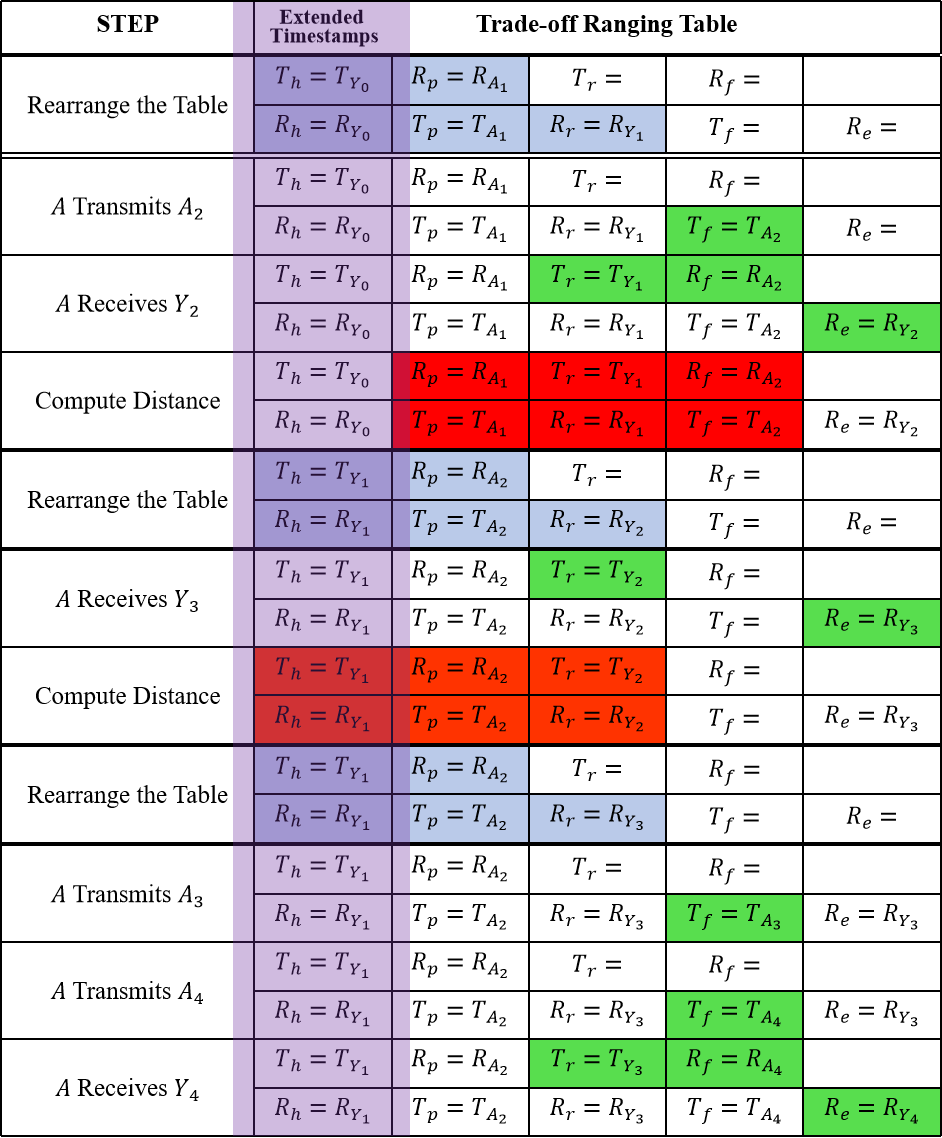
\includegraphics[width=.6\linewidth]{figures/content/chapter3/SwarmRangingSteps.png}
  \caption{采用权衡测距的鲁棒集群测距协议步骤}
  \label{fig:3_9}
\end{figure}

新的测距表结构有效解决了由于时间戳缺失而导致的测距失败问题，其对应的权衡测距方法如算法\ref{alg:trade-off} 所示。

\begin{algorithm}[H]
  \caption{权衡测距算法}
  \label{alg:trade-off}
  \begin{algorithmic}[1]
  
  \While{true}  \Comment{并行任务：发送}
      \State 延时 $P$ 时间
      \ForAll{邻居节点 $Y$}
          \State $Message \gets Message \cup (T_{A_{k-1}}, R_{Y_k})$
      \EndFor
      \State 发送测距报文 $Message$
  \EndWhile
  \Statex
  \Statex \rule{\linewidth}{0.4pt}
  \Statex
  
  \While{true} \Comment{并行任务：接收}
      \State 等待直到接收到测距报文
      \State 设 $Y$ 为报文发送节点的 ID
      \If{在收到的报文中$R_f == \varnothing$}
          \State 对表（AY）：$T_r \gets T_{Y_{k-1}},\; R_f \gets \varnothing,\; R_e \gets R_{Y}$
          \State 利用额外的时间戳计算距离
          \State 更新表：$R_r \gets R_e$（表 AY）
      \Else
          \State 对表（AY）：$T_r \gets T_{Y_{k-1}},\; R_f \gets R_{Y_k},\; R_e \gets R_{Y}$
          \State 计算距离
          \State 更新表：$T_h \gets T_{Y_{k-1}},\; R_h \gets R_{Y_{k-1}},\; R_p \gets R_{A_k},\; T_p \gets T_{A_k},\; R_r \gets R_e$（表 AY）
      \EndIf
  \EndWhile
  
  \end{algorithmic}
\end{algorithm}
      
\subsection{ 最优扰动选择策略}

我们的鲁棒集群测距协议需要在尽可能减少连续测距失败次数的同时，尽量降低权衡测距的发生频率。
因此，本文将该问题建模为一个多目标优化问题，并采用简单加权法来选择合适的抖动参数。
通过在多个目标之间进行协调与折中，实现整体性能的最优。 
在搜索最优抖动参数之前，首先需要对两个目标函数进行归一化处理。
设 $G(W)=1+\frac{1+2W}{W^2+W}$ ,$H(W,P)=P(C)$。
其中，$ G(W)$ 表示连续测距失败次数的度量函数， $H(W,P)$ 表示测距报文不匹配事件发生的概率。
在前文分析中，已将参数$W$ 的取值范围限制为 $\left [ 0, \frac{2}{3}P \right )$。
由于 $G(W)$与 $H(W,P)$ 在该区间内均为单调函数，因此可以分别确定其最大值和最小值。
利用这些极值对目标函数进行归一化，可分别得到归一化后的目标函数 $F_{G}(W)$ 和 $F_{H}(W,P)$。 
据此，本文的多目标优化问题可表示为：


  \begin{equation}
  \begin{aligned}
  \underset{W}{\min }\quad &  \alpha F_{G}(W)+\beta F_{H}(W,P)\\
  \text { s.t. }\quad & 0< W < \frac{2}{3}P\\
  & \alpha + \beta = 1
  \end{aligned}
  \end{equation}

  为有效降低连续测距失败的平均次数，本文将权重系数 $\alpha$设定为 0.9。
  在此权重配置下，得到的最优解 $W^{*}$满足：
  
  \begin{equation}
    \begin{aligned}
    \frac{\partial F(W, P)}{\partial W}=0, F(W,P)=\alpha F_{G}(W)+\beta F_{H}(W) 
    \end{aligned}
    \end{equation} 

根据上述分析，最终可求得最优抖动参数为$W \approx P/10$。
该结果表明，所选取的抖动取值与我们实验章节中的实验结果一致，能够在降低连续测距失败的同时有效抑制测距报文不匹配问题。

\section{自适应协同定位算法}
\subsection{ 系统定义与问题建模}
在进行无人机集群相对定位算法研究之前，本文首先对无人机的机载传感器模型以及无人机相对状态的运动方程进行系统性的介绍，以支撑后续相对定位算法的设计与分析。

\begin{figure}[htbp]
  \centering
  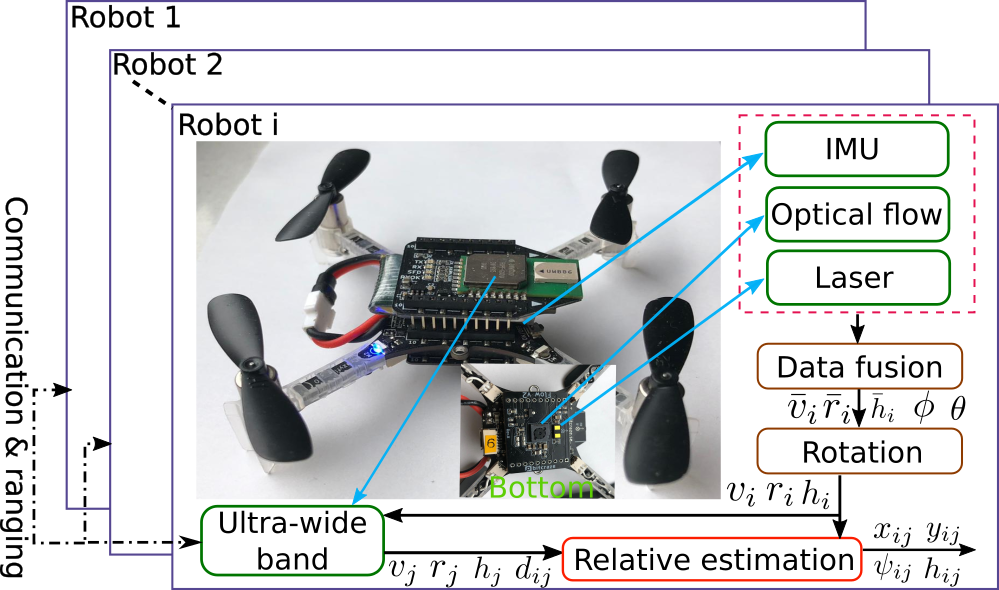
\includegraphics[width=.6\linewidth]{figures/content/chapter3/uwb_sensor.png}
  \caption{无人机集群系统及搭载的机载传感器}
  \label{fig:3_10}
\end{figure}
无人机集群系统中所搭载的传感器如图\ref{fig:3_10}所示。
具体而言，每个无人机均配备惯性测量单元（Inertial Measurement Unit，IMU）、光流传感器以及向下指向的激光测距传感器，用于获取无人机的运动与姿态相关的多源信息。
其中，IMU主要由加速度计和陀螺仪组成，用于测量无人机在本体坐标系下的线加速度和角速度信息。
通过对角速度进行积分可获得无人机的姿态变化情况，而加速度信息则为速度估计和运动建模提供基础，是无人机短时间内高频状态估计的核心传感器。
光流传感器通过观测地面纹理在连续图像帧中的位移变化，估计无人机相对于地面的平移速度，通常用于获取无人机在水平平面内的速度信息。
该传感器不依赖外部定位系统，在近地飞行或低速运动条件下能够提供较为稳定的速度测量，有效抑制仅依赖 IMU 积分所带来的累积误差。
向下指向的激光测距传感器用于测量无人机与地面之间的垂直距离，从而获得高度信息。
该传感器具有测量精度高、响应速度快的特点，可为高度估计提供可靠观测，并与光流传感器协同工作，用于提高速度估计的精度与鲁棒性。

上述传感器数据通过机载滤波器进行融合，得到无人机本体坐标系下的速度、偏航角速率及高度估计值。
随后，利用姿态信息对速度进行坐标变换，将其转换至水平坐标系下，并获得对应的偏航角速率与高度信息。
此外，无人机之间通过超宽带无线通信与测距，基于前文所述的鲁棒集群测距协议实现状态信息的交互与距离测量。
通过融合自身状态估计与来自其他无人机的状态信息，进一步完成对无人机之间相对状态的估计。

为便于分析，本文讨论了任意两个无人机的模型，实现集群协作的前提是无人机$i$需要确定另一个无人机$\{j\mid j\in\mathbb{N}, j\neq i\}$的相对位置。
其中 ， $\mathbb{N}=\{1,2,...,N \}$, $N$是无人机的总数量。
在以无人机$i$为参考坐标系的条件下，定义无人机$j$ 的相对运动状态为 $\boldsymbol{s}_{i j}=\left[\Delta x_{ij}, \Delta y_{i j}, \Delta \theta_{ij}\right]^{\mathrm{T}}$。
结合机载惯性测量单元、光流传感器以及陀螺仪提供的测量信息，可构造系统输入向量$\boldsymbol{u}_{ij}=\left[\boldsymbol{v}_{i}^{\mathrm{T}}, \omega_{i}, \boldsymbol{v}_{j}^{\mathrm{T}}, \omega_{j}\right]^{\mathrm{T}}$。
其中 $\boldsymbol{v}_{i}$​ 与 $\boldsymbol{v}_{j}$分别表示无人机 $i$与 $j$ 在全局参考坐标系下的二维速度向量，
 $\omega_{i}$ ​ 与 $\omega_{j}$ ​ 为对应的偏航角速度。
在牛顿运动定律描述框架下，并仅考虑无人机在水平平面内的平移与偏航运动，可建立无人机对间相对状态的连续时间运动学模型，其表达式为

  \begin{equation}
\dot{\boldsymbol{s}}_{a b}=\boldsymbol{f}\left(\boldsymbol{s}_{a b}, \boldsymbol{u}_{a b}\right)=\left[\begin{array}{c}
\boldsymbol{C}\left(\Delta \theta_{a b}\right) \boldsymbol{v}_{b}-\boldsymbol{v}_{a}-\omega_{a} \boldsymbol{J} \boldsymbol{p}_{a b} \\
\omega_{b}-\omega_{a}
\end{array}\right]
\end{equation}
其中，$\boldsymbol{p}_{a b}=\left[\Delta x_{a b}, \Delta y_{a b}\right]^{\mathrm{T}}$,
$\boldsymbol{C}(\theta)$ 表示二维平面旋转矩阵，$\boldsymbol{J}$ 为二维反对称矩阵，用于刻画角速度对平面位移的耦合影响，其表达式分别为
\begin{equation}
\boldsymbol{C}(\theta)=
\begin{bmatrix}
\cos \theta & -\sin \theta \\
\sin \theta & \cos \theta
\end{bmatrix},
\quad
\boldsymbol{J}=
\begin{bmatrix}
0 & -1 \\
1 & 0  
\end{bmatrix}\text{。}
\end{equation}

基于前文提出的鲁棒集群测距协议，无人机之间可实现相对距离的测量。
设第  $k$  时刻无人机  $i$  与无人机  $j$  的位置分别为
$\boldsymbol{p}_{i, k}=\left[\boldsymbol{x}_{i, k}, \boldsymbol{y}_{i, k}, \boldsymbol{z}_{i, k}\right]^{\mathrm{T}}, \quad \boldsymbol{p}_{j, k}=\left[\boldsymbol{x}_{j, k}, \boldsymbol{y}_{j, k}, \boldsymbol{z}_{j, k}\right]^{\mathrm{T}},$
则无人机  $i$  对无人机  $j$  的距离量测函数可表示为
\begin{equation}
d_{i j, k}=\sqrt{\left(x_{i, k}-x_{j, k}\right)^{2}+\left(y_{i, k}-y_{j, k}\right)^{2}+\left(z_{i, k}-z_{j, k}\right)^{2}} \text{。}
\end{equation}

\subsection{ 自适应扩展卡尔曼滤波算法}
扩展卡尔曼滤波是一类广泛应用于系统状态估计的递推滤波方法，能够处理系统模型中存在的非线性特性以及噪声统计特性未知或近似非高斯的情况。
基于前文构建的无人机状态信息及其运动学模型，本文首先对扩展卡尔曼滤波的预测与校正过程进行说明，随后引入自适应扩展卡尔曼滤波方法，以进一步提升状态估计的鲁棒性与精度。

在采样周期为 $T$ 的条件下，对连续时间模型进行离散化，可得相对状态的离散预测模型为
\begin{equation}
\hat{\mathbf{s}}_{i j, k \mid k-1}=f\left(\hat{\mathbf{s}}_{i j, k-1}, \mathbf{u}_{i j, k-1}\right)=\hat{\mathbf{s}}_{i j, k-1}+\dot{\hat{\mathbf{s}}}_{i j, k-1} T
\end{equation}
其中， $\hat{\mathbf{s}}_{i j, k \mid k-1}$​ 表示在时刻 $ k-1$ 对 $k $时刻的相对状态预测值。

定义相对状态估计误差协方差矩阵为  $\Sigma_{i j, k}$  ，则其预测更新形式为
\begin{equation}
\Sigma_{i j, k \mid k-1}=\Phi_{i j, k-1} \Sigma_{i j, k-1} \Phi_{i j, k-1}^{\mathrm{T}}+\Gamma_{i j, k-1} \Omega_{k-1} \Gamma_{i j, k-1}^{\mathrm{T}}
\end{equation}

其中：
$\Phi_{i j, k}=\left.\frac{\partial f}{\partial \mathbf{s}_{i j}}\right|_{\hat{\mathbf{s}}_{i j, k}}$  为相对运动模型关于状态的雅可比矩阵；
$\Gamma_{i j, k}$  为过程噪声输入矩阵；
$\Omega_{k}$  表示过程噪声协方差矩阵。

在当前预测状态处，对距离观测函数进行一阶泰勒展开，其关于相对状态的雅可比矩阵可表示为
\begin{equation}
J_{i j, k}=\frac{\partial g}{\partial \mathbf{s}_{i j}}=\left[\begin{array}{ccc}
\frac{\Delta x_{i j, k}}{d_{i j, k}} & \frac{\Delta y_{i j, k}}{d_{i j, k}} & 0
\end{array}\right]
\end{equation}
其中，第三项为零是由于距离观测对相对航向角不敏感。

基于预测协方差与观测噪声统计特性，卡尔曼增益矩阵计算如下：
\begin{equation}
G_{i j, k}=\Sigma_{i j, k \mid k-1} J_{i j, k}^{\mathrm{T}}\left(J_{i j, k} \Sigma_{i j, k \mid k-1} J_{i j, k}^{\mathrm{T}}+\Lambda_{k}\right)^{-1}
\end{equation}
其中， $\Lambda_{k}$  为距离测量噪声的协方差矩阵。

在获得距离观测后，相对状态估计可更新为
\begin{equation}
\hat{\mathbf{s}}_{i j, k}=\hat{\mathbf{s}}_{i j, k \mid k-1}+G_{i j, k}\left(d_{i j, k}-g\left(\hat{\mathbf{s}}_{i j, k \mid k-1}\right)\right)
\end{equation}
其中，括号内项为观测残差。

相应的估计误差协方差更新公式为 
\begin{equation}
\begin{array}{l}

\Sigma_{i j, k}=\left(I-G_{i j, k} J_{i j, k}\right) \Sigma_{i j, k \mid k-1}
\end{array}
\end{equation}

在过程噪声协方差矩阵 $\Omega_{k}$ 与观测噪声协方差矩阵$\Lambda_{k}$​ 准确已知的理想条件下，扩展卡尔曼滤波能够为非线性状态空间系统提供线性最小均方误差意义下的最优状态估计。
然而，在实际工程应用中，噪声统计特性往往难以精确获取，一旦 $\Omega_{k}$​ 或 $\Lambda_{k}$ ​ 设定不合理，滤波性能将显著劣化，甚至引发估计不稳定或发散现象。
尤其在微型无人机集群协同定位任务中，由于传感器性能易受环境变化影响，其噪声水平通常具有不确定性和时变性，使得噪声协方差矩阵呈现明显的不确定性与时变特征，从而对定位精度产生不利影响。
因此，研究适用于噪声统计特性不确定条件下的自适应扩展卡尔曼滤波方法具有重要现实意义。 

为进一步阐明噪声协方差矩阵对扩展卡尔曼滤波性能的影响机制，下面对其作用过程进行分析。
当过程噪声协方差矩阵 $\Omega_{k}$​估计不准确时，将首先通过预测协方差更新方程影响相对状态预测误差协方差矩阵$\Sigma_{i j, k\mid ßk−1​}$​的计算结果。
随后，由于卡尔曼增益矩阵$G_{i j, k}$​的求取依赖于$\Sigma_{i j, k\mid ßk−1​}$​，不准确的预测协方差将进一步传递至增益计算过程，最终在状态更新阶段导致相对状态估计$\hat{\mathbf{s}}_{i j, k+1 \mid k}$​偏离最优解，并使对应的估计误差协方差矩阵$\Sigma_{i j, k\mid k−1​}$​失去统计一致性。
因此，过程噪声协方差矩阵$\Omega_{k}$​对滤波性能的影响主要是通过预测误差协方差矩阵$\Sigma_{i j, k\mid ßk−1​}$​间接体现的。

相比之下，观测噪声协方差矩阵$\Lambda_{k}$​ ​的不准确设定将直接作用于卡尔曼增益矩阵$G_{i j, k}$​的计算过程，从而直接影响相对状态的修正结果。
当$\Lambda_{k}$​ ​取值不合理时，将不可避免地导致相对状态估计$\hat{\mathbf{s}}_{i j, k+1 \mid k}$的次优性，并引起估计误差协方差矩阵$\Sigma_{i j, k\mid ßk−1​}$​的不一致问题。
因此，观测噪声协方差矩阵$\Lambda_{k}$​ ​对扩展卡尔曼滤波性能的影响更为直接。

基于上述分析可以看出，相较于难以准确建模的过程噪声协方差矩阵$\Omega_{k}$​，预测误差协方差矩阵$\Sigma_{i j, k\mid k−1​}$​与相对状态估计结果之间具有更加直接的耦合关系，其变化对滤波性能的影响也更为直观，从而为其在线估计与调整提供了可行性。
这一认识构成了本文的主要研究动机。为此，本文提出一种启发式自适应滤波思路，通过对预测误差协方差矩阵$\Sigma_{i j, k\mid k−1​}$​与观测噪声协方差矩阵$\Lambda_{k}$​进行联合估计，避免对过程噪声协方差矩阵$\Omega_{k}$​的直接依赖，并在此基础上设计一种新的自适应扩展卡尔曼滤波算法。

本文旨在利用从初始时刻到当前时刻  $k$  所获得的无人机间距离观测序列$\mathcal{D}_{1: k}=\left\{d_{i j, 1}, d_{i j, 2}, \ldots, d_{i j, k}\right\}$
对预测误差协方差矩阵  $\Sigma_{i j, k \mid k-1}$  以及距离测量噪声协方差矩阵  $\Lambda_{k} $ 进行联合估计。
为此，引入待估参数集合
$\boldsymbol{\theta}_{k} \triangleq\left\{\Sigma_{i j, k \mid k-1}, \Lambda_{k}\right\}$
并基于最大似然准则，通过最大化距离观测序列的对数似然函数$\ell_{\boldsymbol{\theta}_{k}}\left(\mathcal{D}_{1: k}\right) \triangleq \log p_{\boldsymbol{\theta}_{k}}\left(\mathcal{D}_{1: k}\right)$来获得参数估计，即
\begin{equation}
\hat{\boldsymbol{\theta}}_{k}=\arg \max _{\boldsymbol{\theta}_{k}} \ell_{\boldsymbol{\theta}_{k}}\left(\mathcal{D}_{1: k}\right)=\arg \max _{\boldsymbol{\theta}_{k}} \log p_{\boldsymbol{\theta}_{k}}\left(\mathcal{D}_{1: k}\right) 
\end{equation}
其中  $\ell(\cdot)$  表示关于参数  $\boldsymbol{\theta}_{k}$  的对数似然函数。

由于完整联合对数似然函数$\ell_{\boldsymbol{\theta}_{k}}\left(\mathbf{s}_{i j, k}, \mathcal{D}_{1: k}\right) \triangleq \log p_{\boldsymbol{\theta}_{k}}\left(\mathbf{s}_{i j, k}, \mathcal{D}_{1: k}\right)$
相比不完全对数似然函数更易于处理，但相对状态向量  $\mathbf{s}_{i j, k}$  为隐变量，因而上述函数仍不可直接计算。
为此，采用期望最大化思想，通过构造辅助函数
\begin{equation}
\begin{array}{c}
\log p_{\theta_{k}}\left(s_{i j, k}, D_{1: k}\right) \approx \mathcal{Q}\left(\theta_{k}, \theta_{k}^{(l)}\right) \triangleq \mathbb{E}_{s_{i j, k}}\left[\log p_{\theta_{k}}\left(s_{i j, k}, D_{1: k}\right) \mid \theta_{k}^{(l)}, D_{1: k}\right] \\
=\int \log p_{\theta_{k}}\left(s_{i j, k}, D_{1: k}\right) p_{\theta_{k}^{(l)}}\left(s_{i j, k} \mid D_{1: k}\right) d s_{i j, k}
\label{equ:联合概率}
\end{array}
\end{equation}



来近似原对数似然函数，其中  $\theta_{k}^{(l)}$  表示第  $l $ 次迭代的参数估计值。
因此，原始优化问题可转化为$\theta_{k}^{(l+1)} \approx \arg \max _{\theta_{k}} \mathcal{Q}\left(\theta_{k}, \theta_{k}^{(l)}\right)$ 。

下面进行可行性证明：
由联合概率密度函数与条件概率密度函数之间的关系可知，辅助函数的定义式 \ref{equ:联合概率} 可以重新写为：

\begin{equation}
\begin{array}{c}
\mathcal{Q}\left(\theta_{k}, \theta_{k}^{(l)}\right)=\int \log p_{\theta_{k}}\left(s_{i j, k} \mid D_{1: k}\right) p_{\theta_{k}^{(l)}}\left(s_{i j, k} \mid D_{1: k}\right) d s_{i j, k} \\
+\int \log p_{\theta_{k}}\left(D_{1: k}\right) p_{\theta_{k}^{(l)}}\left(s_{i j, k} \mid D_{1: k}\right) d s_{i j, k} \\
=\int \log p_{\theta_{k}}\left(s_{i j, k} \mid D_{1: k}\right) p_{\theta_{k}^{(l)}}\left(s_{i j, k} \mid D_{1: k}\right) d s_{i j, k}+\ell_{\theta_{k}}\left(D_{1: k}\right)
\end{array}
\end{equation}

在上式中令 $\theta_{k}=\theta_{k}^{(l)}$ ，可得：
\begin{equation}
\mathcal{Q}\left(\theta_{k}^{(l)}, \theta_{k}^{(l)}\right)=\int \log p_{\theta_{k}^{(l)}}\left(s_{i j, k} \mid D_{1: k}\right) p_{\theta_{k}^{(l)}}\left(s_{i j, k} \mid D_{1: k}\right) d s_{i j, k}+\ell_{\theta_{k}^{(l)}}\left(D_{1: k}\right)
\end{equation}
因此，
\begin{equation}
 \ell_{\theta_{k}}\left(D_{1: k}\right)-\ell_{\theta_{k}^{(l)}}\left(D_{1: k}\right)=\mathcal{Q}\left(\theta_{k}, \theta_{k}^{(l)}\right)-\mathcal{Q}\left(\theta_{k}^{(l)}, \theta_{k}^{(l)}\right) \\
\int \log \frac{p_{\theta_{k}}\left(s_{i j, k} \mid D_{1: k}\right)}{p_{\theta_{k}^{(l)}}\left(s_{i j, k} \mid D_{1: k}\right)} p_{\theta_{k}^{(l)}}\left(s_{i j, k} \mid D_{1: k}\right) d s_{i j, k}
\end{equation}
由于右侧积分项为 Kullback–Leibler 散度\cite{huang2017novel, tzikas2008variational}，其值非负，因此可得不等式
\begin{equation}
\ell_{\theta_{k}}\left(D_{1: k}\right)-\ell_{\theta_{k}^{(l)}}\left(D_{1: k}\right) \geq \mathcal{Q}\left(\theta_{k}, \theta_{k}^{(l)}\right)-\mathcal{Q}\left(\theta_{k}^{(l)}, \theta_{k}^{(l)}\right) .
\end{equation}
只要保证
$\mathcal{Q}\left(\theta_{k}^{(l+1)}, \theta_{k}^{(l)}\right) \geq \mathcal{Q}\left(\theta_{k}^{(l)}, \theta_{k}^{(l)}\right),$
即可得到$\ell_{\theta_{k}^{(l+1)}}\left(D_{1: k}\right) \geq \ell_{\theta_{k}^{(l)}}\left(D_{1: k}\right),$
从而证明该方法在每次迭代中均能提高对数似然函数值，算法具有可行性与单调收敛性。

下文将基于期望最大化算法进行证明，首先在期望步骤方面：对辅助函数  $\mathcal{Q}\left(\theta_{k}, \theta_{k}^{(l)}\right)$  进行简化。
根据贝叶斯定理，有
\begin{equation}
p_{\theta_{k}}\left(s_{i j, k}, D_{1: k}\right)=p_{\theta_{k}}\left(d_{i j, k} \mid s_{i j, k}\right) p_{\theta_{k}}\left(s_{i j, k} \mid D_{1: k-1}\right) p\left(D_{1: k-1}\right) .
\end{equation}

在扩展卡尔曼滤波框架下，上式中各项可近似表示为高斯分布：
\begin{equation}
\begin{array}{c}
p_{\theta_{k}}\left(s_{i j, k} \mid D_{1: k-1}\right)=\mathcal{N}\left(s_{i j, k} ; \hat{s}_{i j, k \mid k-1}, \Sigma_{i j, k \mid k-1}\right) \\
p_{\theta_{k}}\left(d_{i j, k} \mid s_{i j, k}\right)=\mathcal{N}\left(d_{i j, k} ; g\left(s_{i j, k}\right), \Lambda_{k}\right)
\end{array}
\end{equation}

由于  $p\left(D_{1: k-1}\right)$  与参数  $\theta_{k}$  无关，因此在最大化过程中可视为常数项。
于是，对数联合概率密度函数可写为
\begin{equation}
\log p_{\theta_{k}}\left(s_{i j, k}, D_{1: k}\right)=-\frac{1}{2} \log \left|\Lambda_{k}\right|-\frac{1}{2}\left(d_{i j, k}-g\left(s_{i j, k}\right)\right)^{T} \Lambda_{k}^{-1}\left(d_{i j, k}-g\left(s_{i j, k}\right)\right)+c_{\theta_{k}} .
\end{equation}

进一步近似后验分布为
\begin{equation}
p_{\theta_{k}}^{(l)}\left(s_{i j, k} \mid D_{1: k}\right)=\mathcal{N}\left(s_{i j, k} ; \hat{s}_{i j, k \mid k}^{(l+1)}, \Sigma_{i j, k \mid k}^{(l+1)}\right) .
\end{equation}
将上述结果代入辅助函数，可得

\begin{equation}
\mathcal{Q}\left(\theta_{k}, \theta_{k}^{(l)}\right)=-\frac{1}{2} \log \left|\Lambda_{k}\right|-\frac{1}{2} \operatorname{tr}\left(A_{k} \Lambda_{k}^{-1}\right)-\frac{1}{2} \log \left|\Sigma_{i j, k \mid k-1}\right|-\frac{1}{2} \operatorname{tr}\left(B_{k} \Sigma_{i j, k \mid k-1}^{-1}\right)+c_{\theta_{k}},
\end{equation}

其中
\begin{equation}
\begin{aligned}
A_{k} & =\int\left[d_{i j, k}-g\left(s_{i j, k}\right)\right]\left[d_{i j, k}-g\left(s_{i j, k}\right)\right]^{T} \mathcal{N}\left(s_{i j, k} ; \hat{s}_{i j, k \mid k}^{(l+1)}, \Sigma_{i j, k \mid k}^{(l+1)}\right) d s_{i j, k} \\
B_{k} & =\int\left(s_{i j, k}-\hat{s}_{i j, k \mid k-1}\right)\left(s_{i j, k}-\hat{s}_{i j, k \mid k-1}\right)^{T} \mathcal{N}\left(s_{i j, k} ; \hat{s}_{i j, k \mid k}^{(l+1)}, \Sigma_{i j, k \mid k}^{(l+1)}\right) d s_{i j, k}
\end{aligned}
\end{equation}

根据上文定义的距离观测模型，在当前迭代估计点 $\hat{s}_{i j, k}^{(l+1)}$处对观测函数进行一阶泰勒展开，可得
\begin{equation}
g\left(s_{i j, k}\right) \approx g\left(\hat{s}_{i j, k}^{(l+1)}\right)+J_{i j, k}^{(l+1)}\left(s_{i j, k}-\hat{s}_{i j, k}^{(l+1)}\right)
\end{equation}
其中,$J_{i j, k}^{(l+1)}=\left.\frac{\partial g}{\partial s_{i j}}\right|_{\hat{s}_{i j, k}^{(l+1)}}$表示观测函数在  $\hat{s}_{i j, k}^{(l+1)}$  处的雅可比矩阵。
根据距离函数的偏导计算，可得$J_{i j, k}^{(l+1)}=\left[\begin{array}{ll}
\frac{\Delta x_{i j, k}}{d_{i j, k}} & \frac{\Delta y_{i j, k}}{d_{i j, k}}
\end{array}\right]$
利用线性化的结果对$A_{k} $和$B_{k}$进行详细的推导计算：
利用上述的线性化结果代入可得
\begin{equation}
\begin{aligned}
A_{i j, k}= & \int\left[d_{i j, k}-g\left(\hat{s}_{i j, k \mid k}^{(l+1)}\right)-J_{i j, k}^{(l+1)}\left(s_{i j, k}-\hat{s}_{i j, k \mid k}^{(l+1)}\right)\right] \\
& {\left[d_{i j, k}-g\left(\hat{s}_{i j, k \mid k}^{(l+1)}\right)-J_{i j, k}^{(l+1)}\left(s_{i j, k}-\hat{s}_{i j, k \mid k}^{(l+1)}\right)\right]^{T} } \\
& \mathcal{N}\left(s_{i j, k} ; \hat{s}_{i j, k \mid k}^{(l+1)}, \Sigma_{i j, k \mid k}^{(l+1)}\right) d s_{i j, k}
\end{aligned}
\end{equation}

利用高斯积分公式可得
\begin{equation}
A_{i j, k}=\left[d_{i j, k}-g\left(\hat{s}_{i j, k \mid k}^{(l+1)}\right)\right]\left[d_{i j, k}-g\left(\hat{s}_{i j, k \mid k}^{(l+1)}\right)\right]^{T}+J_{i j, k}^{(l+1)} \Sigma_{i j, k \mid k}^{(l+1)}\left(J_{i j, k}^{(l+1)}\right)^{T}
\end{equation}

同理可得：
\begin{equation}
\begin{aligned}
B_{i j, k}=\int & \left(s_{i j, k}-\hat{s}_{i j, k \mid k}^{(l+1)}+\hat{s}_{i j, k \mid k}^{(l+1)}-\hat{s}_{i j, k \mid k-1}\right) \\
& \left(s_{i j, k}-\hat{s}_{i j, k \mid k}^{(l+1)}+\hat{s}_{i j, k \mid k}^{(l+1)}-\hat{s}_{i j, k \mid k-1}\right)^{T} \\
& \mathcal{N}\left(s_{i j, k} ; \hat{s}_{i j, k \mid k}^{(l+1)}, \Sigma_{i j, k \mid k}^{(l+1)}\right) d s_{i j, k}
\end{aligned}
\end{equation}

最终得到
\begin{equation}
B_{i j, k}=\Sigma_{i j, k \mid k}^{(l+1)}+\left(\hat{s}_{i j, k \mid k}^{(l+1)}-\hat{s}_{i j, k \mid k-1}\right)\left(\hat{s}_{i j, k \mid k}^{(l+1)}-\hat{s}_{i j, k \mid k-1}\right)^{T}
\end{equation}

在最大化步骤中，通过最大化  $\mathcal{Q}\left(\theta_{k}, \theta_{k}^{(l)}\right)$  对参数  $\theta_{k}$  进行更新，即
\begin{equation}
\left.\frac{\partial \mathcal{Q}\left(\theta_{k}, \theta_{k}^{(l)}\right)}{\partial \theta_{k}}\right|_{\theta_{k}=\theta_{k}^{(l+1)}}=0 .
\end{equation}

由于$\theta_{k}=\left\{\Sigma_{i j, k \mid k-1}, \Lambda_{k}\right\},$上述条件可分别转化为
\begin{equation}
\frac{\partial \mathcal{Q}}{\partial \Sigma_{i j, k \mid k-1}}=0, 
\frac{\partial \mathcal{Q}}{\partial \Lambda_{k}}=0 .
\end{equation}


偏导数$\frac{\partial \mathcal{Q}\left(\theta_{k}, \theta_{k}^{(l)}\right)}{\partial \Sigma_{i j, k \mid k-1}}$
和$\frac{\partial \mathcal{Q}\left(\theta_{k}, \theta_{k}^{(l)}\right)}{\partial \Lambda_{k}}$
可以被计算如下：
\begin{equation}
\begin{array}{c}
\frac{\partial \mathcal{Q}\left(\theta_{k}, \theta_{k}^{(l)}\right)}{\partial \Sigma_{i j, k \mid k-1}}=-\frac{1}{2} \Sigma_{i j, k \mid k-1}^{-1}+\frac{1}{2} \Sigma_{i j, k \mid k-1}^{-1} B_{k} \Sigma_{i j, k \mid k-1}^{-1} \\
\frac{\partial \mathcal{Q}\left(\theta_{k}, \theta_{k}^{(l)}\right)}{\partial \Lambda_{k}}=-\frac{1}{2} \Lambda_{k}^{-1}+\frac{1}{2} \Lambda_{k}^{-1} A_{k} \Lambda_{k}^{-1}
\end{array}
\end{equation}

因此求解可得更新公式
\begin{equation}
\Sigma_{i j, k \mid k-1}^{(l+1)}=B_{k},  \Lambda_{k}^{(l+1)}=A_{k}
\end{equation}

\begin{figure}[htbp]
  \centering
  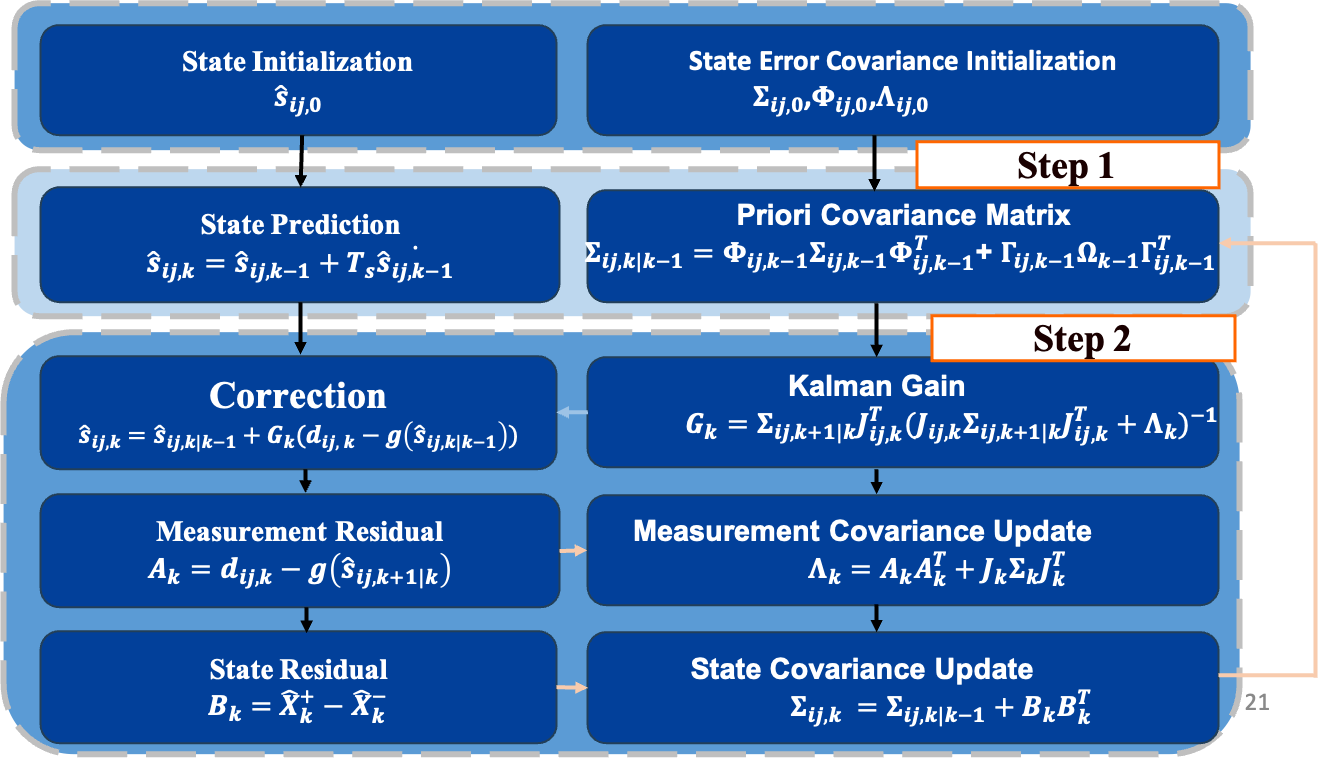
\includegraphics[width=.8\linewidth]{figures/content/chapter3/自适应EKF算法流程.png}
  \caption{自适应扩展卡尔曼滤波算法流程图}
  \label{fig:3_11}
\end{figure}

上述为所提出自适应扩展卡尔曼滤波算法的可行性证明，算法伪代码如算法\ref{alg:AEKF_UAV} 所示。


针对传统扩展卡尔曼滤波在实际应用中对过程噪声协方差和观测噪声协方差依赖性较强、相关参数难以准确获取的问题，本章在原有滤波框架基础上，引入期望最大化算法构建参数自适应估计机制。
具体而言，将预测误差协方差矩阵与观测噪声协方差矩阵视为待估参数。在期望步中，通过计算完全数据对数似然函数的条件期望来估计隐藏变量的统计特性；
在最大化步中，对上述期望函数进行极大化求解，从而得到参数的更新表达式。
基于该过程，推导获得了预测协方差矩阵和观测噪声协方差矩阵的递推更新公式，并将其嵌入扩展卡尔曼滤波的迭代计算流程中，形成一种自适应扩展卡尔曼滤波算法。

通过上述方法，所提出的自适应扩展卡尔曼滤波能够在噪声统计特性未知或存在不确定性的情况下，实现对无人机相对状态的稳定估计。
同时，该方法能够根据观测数据动态调整噪声参数，提高滤波算法对环境变化的适应能力，从而为无人机协同定位与编队控制提供一种有效且鲁棒的状态估计方案。


\begin{algorithm}[H]
\caption{基于期望最大化算法的自适应扩展卡尔曼滤波算法}
\label{alg:AEKF_UAV}

\begin{algorithmic}

\State \textbf{输入：}  $\hat{s}_{ij,k-1|k-1}$， $\Sigma_{ij,k-1|k-1}$，$\Omega_{k-1}$, $\mathbf{u}_{ij, k}$， $g(s_{ij,k})$，
 $d_{ij,k}$，$\tilde{\Sigma}_{ij,k-1}$，
$\tilde{\Lambda}_{k-1}$，$N$

\State \textbf{时间更新：}

\State 1. $\hat{\mathbf{s}}_{i j, k \mid k-1}=\hat{\mathbf{s}}_{i j, k-1}+\dot{\hat{\mathbf{s}}}_{i j, k-1} T$


\State 2. $\Sigma_{i j, k \mid k-1}=\Phi_{i j, k-1} \Sigma_{i j, k-1} \Phi_{i j, k-1}^{\mathrm{T}}+\Gamma_{i j, k-1} \Omega_{k-1} \Gamma_{i j, k-1}^{\mathrm{T}}$

\State \textbf{迭代测量更新：}

\State 3. 初始化：$\Sigma^{(0)}_{ij,k|k-1} = \tilde{\Sigma}_{ij,k|k-1},\quad \Lambda^{(0)}_k = \tilde{\Lambda}_k$, $\hat{s}^{(0)}_{ij,k|k} = \hat{s}_{ij,k|k-1}$

\For{$l = 0 : N - 1$}

\State 给定 $\Sigma^{(l)}_{ij,k|k-1}$、$\Lambda^{(l)}_k$ 和 $\hat{s}^{(l)}_{ij,k|k}$，更新 $\hat{s}^{(l+1)}_{ij,k|k}$ 和 $\Sigma^{(l+1)}_{ij,k|k}$：

\State 4. 计算雅可比矩阵
\[
J^{(l)}_{ij,k} =
\begin{bmatrix} 
\dfrac{\Delta x^{(l)}_{ij,k|k}}{\sqrt{(\Delta x^{(l)}_{ij,k|k})^2 + (\Delta y^{(l)}_{ij,k|k})^2}}, &
\dfrac{\Delta y^{(l)}_{ij,k|k}}{\sqrt{(\Delta x^{(l)}_{ij,k|k})^2 + (\Delta y^{(l)}_{ij,k|k})^2}}
\end{bmatrix}
\]

\State 5. 计算卡尔曼增益: $G^{(l+1)}_{ij,k} =
\Sigma^{(l)}_{ij,k|k-1}(J^{(l)}_{ij,k})^T
\left(
J^{(l)}_{ij,k}\Sigma^{(l)}_{ij,k|k-1}(J^{(l)}_{ij,k})^T + \Lambda^{(l)}_k
\right)^{-1}$

\State 6. 更新状态估计:$
\hat{s}^{(l+1)}_{ij,k|k}
=
\hat{s}_{ij,k|k-1}
+
G^{(l+1)}_{ij,k}
\left(
d_{ij,k}
-
g(\hat{s}^{(l)}_{ij,k|k})
-
J^{(l)}_{ij,k}
(\hat{s}_{ij,k|k-1} - \hat{s}^{(l)}_{ij,k|k})
\right)
$

\State 7. 更新后验协方差:$
\Sigma^{(l+1)}_{ij,k|k}
=
\Sigma^{(l)}_{ij,k|k-1}
-
G^{(l+1)}_{ij,k}
J^{(l)}_{ij,k}
\Sigma^{(l)}_{ij,k|k-1}
$

\State 8. 计算更新后的雅可比矩阵
\[
J^{(l+1)}_{ij,k} =
\begin{bmatrix} 
\dfrac{\Delta x^{(l+1)}_{ij,k|k}}{\sqrt{(\Delta x^{(l+1)}_{ij,k|k})^2 + (\Delta y^{(l+1)}_{ij,k|k})^2}}, &
\dfrac{\Delta y^{(l+1)}_{ij,k|k}}{\sqrt{(\Delta x^{(l+1)}_{ij,k|k})^2 + (\Delta y^{(l+1)}_{ij,k|k})^2}}
\end{bmatrix}
\]

\State 9. 计算观测相关矩阵:
$A_k =
\left[d_{ij,k} - g(\hat{s}^{(l+1)}_{ij,k|k})\right]
\left[d_{ij,k} - g(\hat{s}^{(l+1)}_{ij,k|k})\right]^T
+
J^{(l+1)}_{ij,k}
\Sigma^{(l+1)}_{ij,k|k}
(J^{(l+1)}_{ij,k})^T$


\State 10. 计算状态相关矩阵:
\[B_k =
\Sigma^{(l+1)}_{ij,k|k}
+
(\hat{s}^{(l+1)}_{ij,k|k} - \hat{s}_{ij,k|k-1})
(\hat{s}^{(l+1)}_{ij,k|k} - \hat{s}_{ij,k|k-1})^T
\]

\State 11. 更新参数:
$\Sigma^{(l+1)}_{ij,k|k-1} = B_k,\quad
\Lambda^{(l+1)}_k = A_k$


\EndFor

\State 12. 输出最终估计结果
\[
\hat{s}_{ij,k|k} = \hat{s}^{(N)}_{ij,k|k},\quad
\Sigma_{ij,k|k} = \Sigma^{(N)}_{ij,k|k},\quad
\hat{\Sigma}_{ij,k|k-1} = \Sigma^{(N)}_{ij,k|k-1},\quad
\hat{\Lambda}_k = \Lambda^{(N)}_k
\]

\State \textbf{输出：} 当前时刻后验状态估计 $\hat{s}_{ij,k|k}$，后验协方差 $\Sigma_{ij,k|k}$，
预测协方差估计 $\hat{\Sigma}_{ij,k|k-1}$ 和观测噪声协方差估计 $\hat{\Lambda}_k$

\end{algorithmic}

\end{algorithm}

\section{实验设置与结果分析}

本节通过真实无人机集群实验，对所提出的鲁棒集群测距协议以及自适应协同定位算法的实际性能进行验证，并进一步展示在仅依赖相对定位信息条件下的大规模无人机集群自主飞行能力。

实验平台采用商业微型四旋翼无人机 Crazyflie 2.1 构建无人机集群系统。
如图\ref{fig:3_12}所示，每架无人机均搭载多种传感器模块，用于实现相对定位与集群飞行。具体配置如下：

\begin{figure}[htbp]
  \centering
  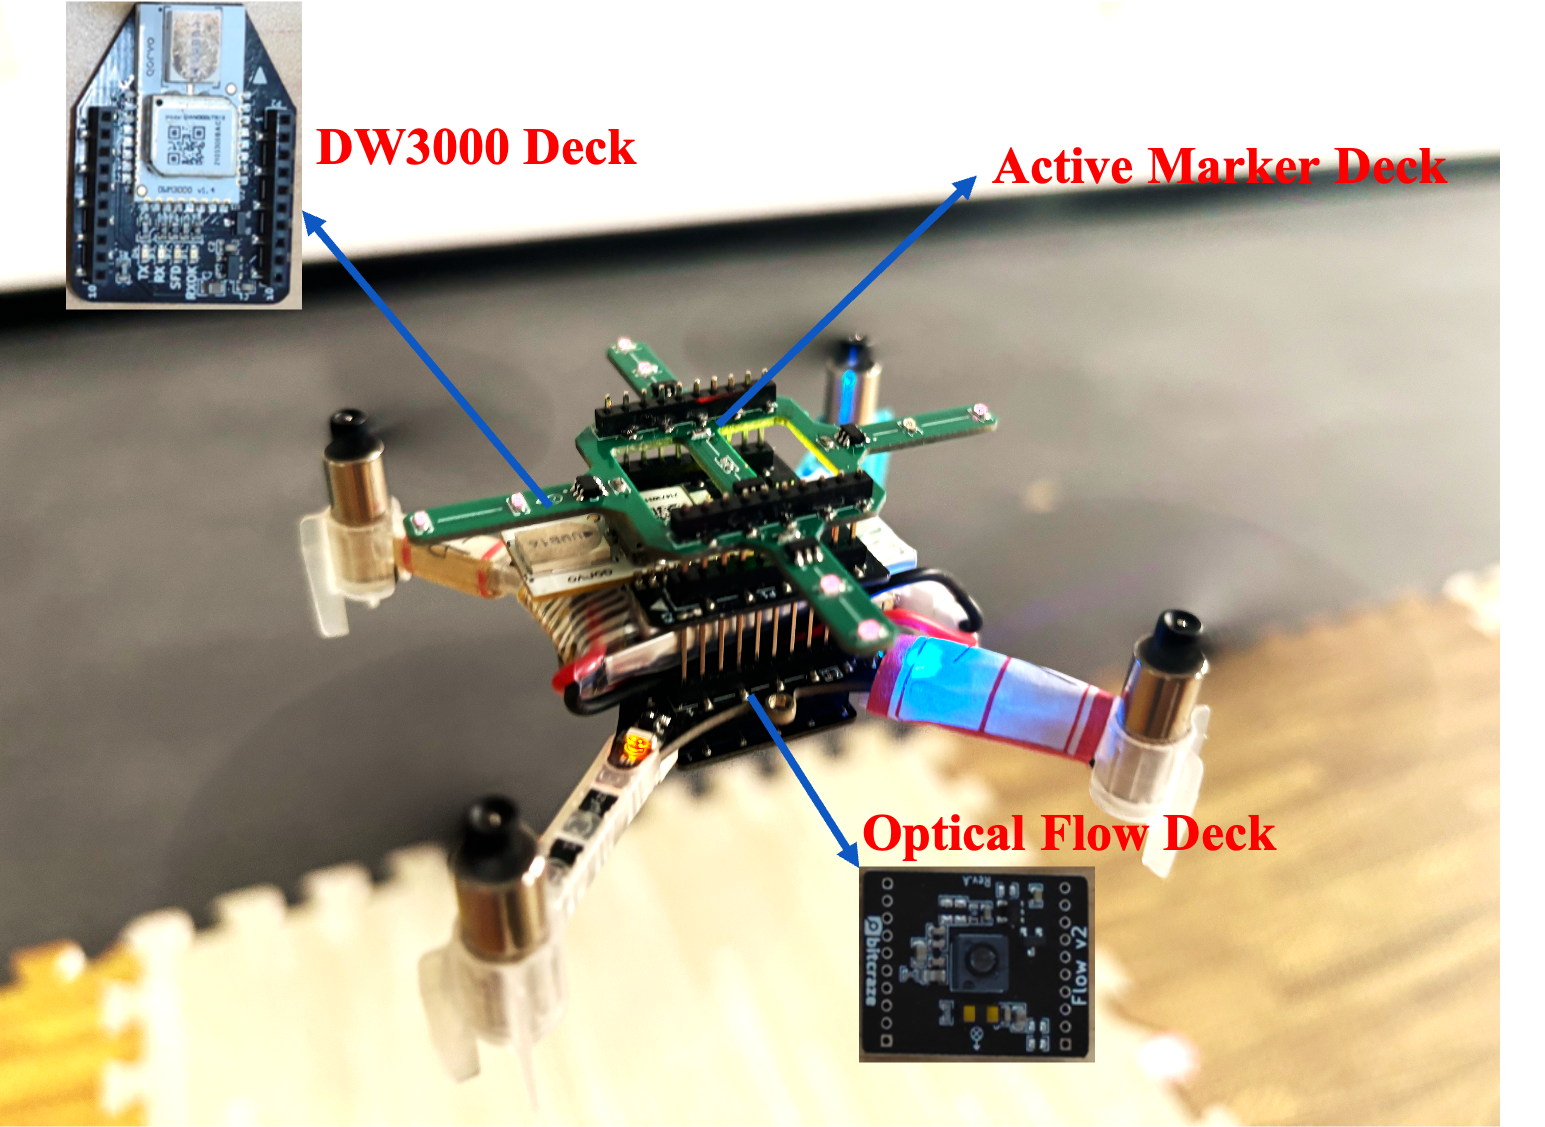
\includegraphics[width=.6\linewidth]{figures/content/chapter3/crazyflie_drone_flo_uwb.pdf}
  \caption{实验用到的无人机以及传感器}
  \label{fig:3_12}
\end{figure}

\begin{itemize}
\item 惯性测量单元（IMU）：包含三轴加速度计和三轴陀螺仪，用于获取无人机的姿态和运动信息。

\item 光流传感器模块（Optical Flow Deck）：由 VL53L1x 激光高度传感器和 PMW3901 光流传感器组成，可提供最高 100 Hz 的速度测量数据。

\item 超宽带测距模块（UWB3000 Deck）：基于 DWM3000 UWB芯片，用于无人机之间的距离测量，是实现集群相对定位的重要信息来源。

\item 主动标记模块（Active Marker Deck）：由高功率 LED 构成，可设置不同 ID，从而在运动捕捉系统中实现大量刚体目标的唯一识别，避免使用大量反光标记。
\end{itemize}

无人机系统采用STM32F4微控制器作为主处理单元，主频 168 MHz，片上内存 192 KB。
在该处理器上同时运行的核心算法模块包括：集群测距协议、自适应相对定位算法与飞行控制算法。

所有实验均在 6 m × 6 m 的室内实验场地中进行，如图\ref{fig:3_13}所示。
为了获得精确的参考数据，实验系统使用 OptiTrack运动捕捉系统实时获取每架无人机的真实位置与偏航角。
该系统提供高精度位姿信息，用于记录实验真实轨迹并在实验后进行性能评估与误差分析
需要说明的是，运动捕捉系统数据仅用于实验结果验证和后期数据分析，并未参与算法的在线估计过程。无人机在实际运行过程中仅依赖机载传感器和UWB测距信息进行相对定位与协同飞行。

\begin{figure}[htbp]
  \centering
  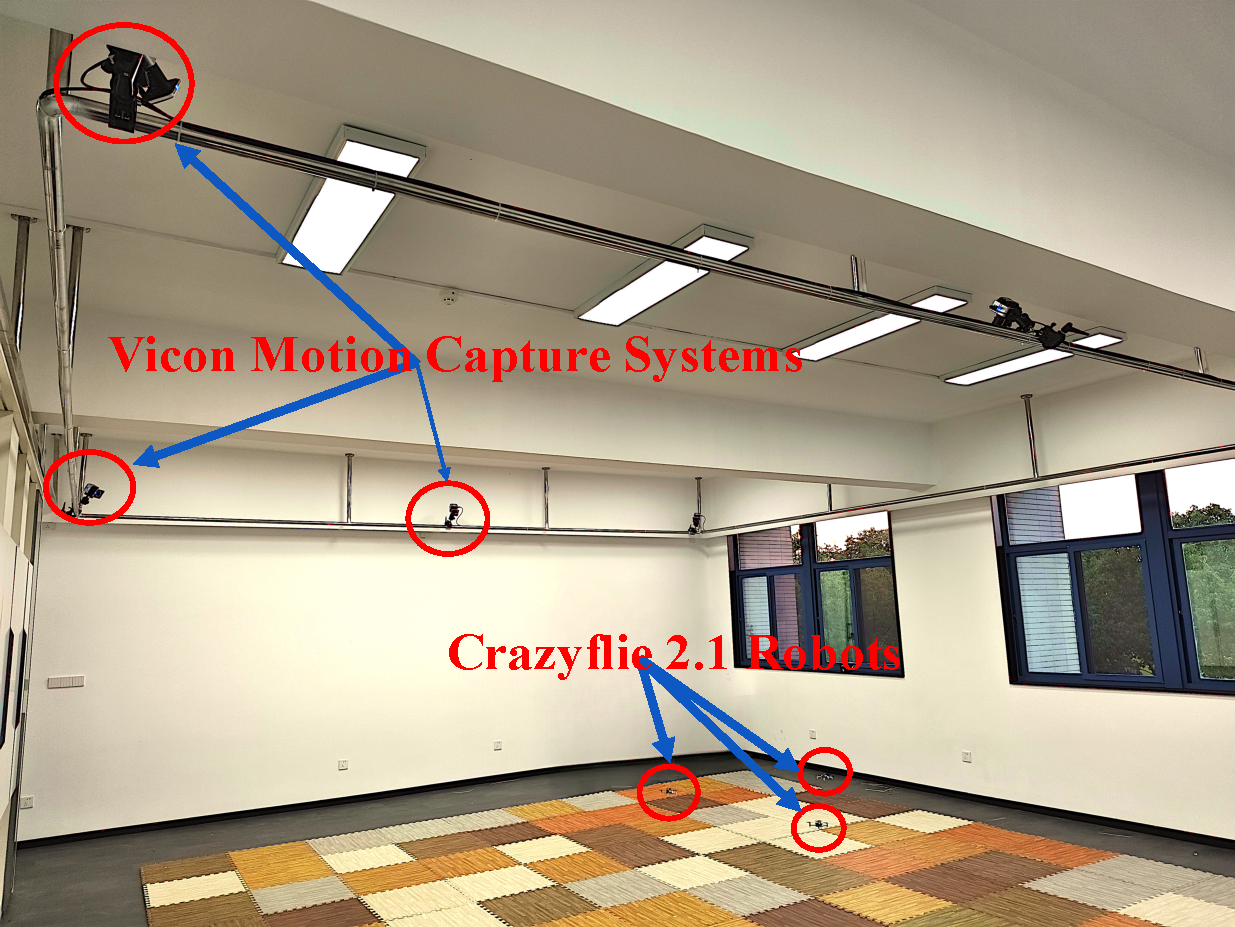
\includegraphics[width=.6\linewidth]{figures/content/chapter3/environment.pdf}
  \caption{实验场地}
  \label{fig:3_13}
\end{figure}


通过大量真实飞行实验验证，所提出的鲁棒集群测距协议能够在动态密集的无人机网络环境中提供稳定、高效的距离更新，从而显著提升自适应协同定位算法在大规模无人机集群中的定位性能与鲁棒性。

\subsection{  DW3000的时钟偏移与处理时间验证}

为研究两块 DW3000 芯片之间的时钟偏差，本小节设计并开展了一组实验。
在该实验中，两个无人机同时按照 10 ms 的测距周期执行周期性测距任务，并记录了 10,000 次消息发送的时间戳。

实验结果表明，两无人机的平均测距周期分别为 9.981966 ms 和 9.988414 ms。
由此可以得到，两无人机发送报文的时间戳差值（即两块 DW3000 芯片之间的相对时钟偏差）约为 0.00645 ms（即 9.988414 ms − 9.981966 ms）。
尽管该时钟偏差数值较小，但随着时间累积会导致同步误差的逐渐增大。
具体而言，在约 15.5 s 之后（计算方式为 10 ms x 10ms/ 0.00645 ms），两无人机将进入连续测距失败阶段。

此外，还开展了另一组实验以评估 DW3000 芯片处理报文的时间开销。
在该实验中，通过计算无人机发送报文后与下一次接收报文的时间戳差值，连续两次接收报文时间戳之间的差值来估计芯片在发送和接收报文过程中的处理时间。
实验过程中未为无人机设置随机化等待时间。
在时钟偏差的影响下，所测得的时间差会从一个最小值逐渐增加至最大值，其中最小值对应于芯片完成一次报文发送和接收所需的处理时间，而最大值对应于测距周期。

实验结果如 表 \ref{tab:timing} 所示。结果表明，即使在 26 架机器人组成的集群系统中，单条测距消息的处理时间仍然 小于 1 ms。
实验数据可以进一步被用于第 \ref{sec:sim_performence}节中的仿真实验参数设置。

\begin{table}[h]
\centering
\caption{不同规模无人机集群中的报文收发处理时间}
\label{tab:timing}
\begin{tabular}{|c|c|c|c|c|}
\hline
\textbf{集群数量} & 2   & 10  & 18  & 26  \\ \hline
\textbf{报文发送处理时间}               & 0.167ms & 0.259ms & 0.312ms & 0.389ms \\ \hline
\textbf{报文接收处理时间}               & 0.339ms & 0.441ms & 0.548ms & 0.662ms \\ \hline
\end{tabular}
\end{table}
\subsection{ 大规模集群测距的仿真鲁棒性分析}
\label{sec:sim_performence}

前文已从理论角度分析了两架无人机执行鲁棒集群测距协议时的性能表现。
然而，在大规模无人机集群中，随着参与无人机数量的增加，集群内部的通信与测距交互显著增多，同时信号干扰的可能性也随之提高，从而使系统复杂度大幅上升。
因此，在包含大量无人机参与的场景下，对鲁棒集群测距协议性能进行建模与预测成为一项具有挑战性的任务。
为此，本节通过构建仿真模型，对大规模集群环境下该协议的性能进行分析。

\begin{algorithm}[htbp]
\caption{大规模集群收发包仿真算法}
\label{alg:sim_alg}
\setlength{\baselineskip}{0.98\baselineskip}
\textbf{Input:} $N, P, W, D, I$ \\
\textbf{Output:} $recv\_packets$ \\
$packets = generateTxPacket(N, P, W, D)$ \\
计算 $tx, rx$ by Eq.(\ref{eq:txrxdiff}) and (\ref{eq:rxtxdiff}) \\
初始化 $recv\_packets = [\,]$ and $seq = 1$ \\
\textbf{for} $pkt$ in $packets$ \textbf{do} \\
\hspace*{1em} \textbf{if} $pkt.id == I$ \textbf{then} \\
\hspace*{1em} $tran\_Start = pkt.tx,\; tran\_End = pkt.tx + tx,\; seq++$ \\
\hspace*{1em} \textbf{continue} \\
\hspace*{1em} \textbf{end if} \\
\hspace*{1em} \textbf{if} $pkt.tx \ge rece\_Start$ and $pkt.tx \le rece\_End$ \textbf{then} \\
\hspace*{1em} \textbf{continue} \\
\hspace*{1em} \textbf{end if} \\
\hspace*{1em} \textbf{if} $pkt.tx \ge tran\_Start$ and $pkt.tx \le tran\_End$ \textbf{then} \\
\hspace*{1em} \textbf{continue} \\
\hspace*{1em} \textbf{end if} \\
\hspace*{1em} \textbf{if} $packets[I][seq].tx \le pkt.tx \le packets[I][seq].tx + tx$ \textbf{then} \\
\hspace*{1em} \textbf{continue} \\
\hspace*{1em} \textbf{end if} \\
\hspace*{1em} $rece\_Start = pkt.tx + tx,\; rece\_End = pkt.tx + rx$ \\
\hspace*{1em} $recv\_packets.append(pkt)$ \\
\textbf{end for}

\end{algorithm}

仿真工具的核心功能是模拟目标无人机发送数据包以及从邻居无人机接收数据包的过程，并考虑数据报文在传输过程中可能发生的丢失情况。
该仿真工具的输入参数包括：用于仿真的无人机数量 $N$、测距周期的平均值$P$、测距周期的抖动范围 $W$、
目标无人机编号 $I$，以及总仿真时长$D$。

在仿真过程中，一个关键挑战在于如何合理地设置各无人机之间的时钟偏差。
为此，利用真实实验中测得的测距周期的均值和方差，为每架无人机随机生成一系列数据报文的发送时间戳，以模拟真实系统中的时钟漂移特性。

为了模拟目标无人机从邻居无人机接收报文的过程，需要对报文发送与接收过程中的处理时间进行精确建模。
当接收操作与另一接收操作或发送操作之间的时间间隔过小时，接收过程可能发生失败。
因此，在仿真模型中需要考虑报文发送与接收处理时间之间的约束关系。

此外，为了刻画报文大小与处理时间之间的关系，采用线性回归分析方法建立相应的线性模型。该线性函数可以表示为：
\begin{align}
tx &= tx\_k * packetSize + tx\_b, \label{eq:txrxdiff}\\
rx &= rx\_k * packetSize + rx\_b, \label{eq:rxtxdiff}
\end{align}
其中，模型参数通过最小二乘法进行估计，不同数据包大小对应的处理时间如表\ref{tab:timing}所示。

该算法的核心思想是判断无人机是否能够成功接收数据包。
仿真核心部分的伪代码如算法 \ref{alg:sim_alg}所示。
在仿真过程中，按照时间顺序依次遍历每一个数据包，并根据模拟得到的处理时间判断该数据包是否应被丢弃。
如果某一邻居无人机在其自身发送或接收报文的处理时间内发送数据包，则该数据包将被判定为丢失。
通过对无人机集群中的报文发送与接收过程进行仿真，并结合前述分析，可以进一步判断系统中是否出现连续测距失败或权衡测距的情况。

图 \ref{fig:3_14}展示了仿真实验结果。
仿真分别在 25、50、75 和 100 架无人机组成的集群规模下进行，仿真时长为 200 s，平均测距周期设置为 100 ms。
实验结果表明，随着集群规模的增大，由于报文大小增加以及丢失概率上升，系统中出现连续测距失败的次数也随之增加。
此外，随着随机化程度的提高，连续测距失败的平均次数呈现下降趋势。
值得注意的是，权衡测距的比例基本不受集群规模影响，而仅与随机数的选择有关。
上述结果验证了该协议在大规模集群场景下的可扩展性，并为其在实际系统中的部署提供了参考依据。

\begin{figure}[h]
\centerline{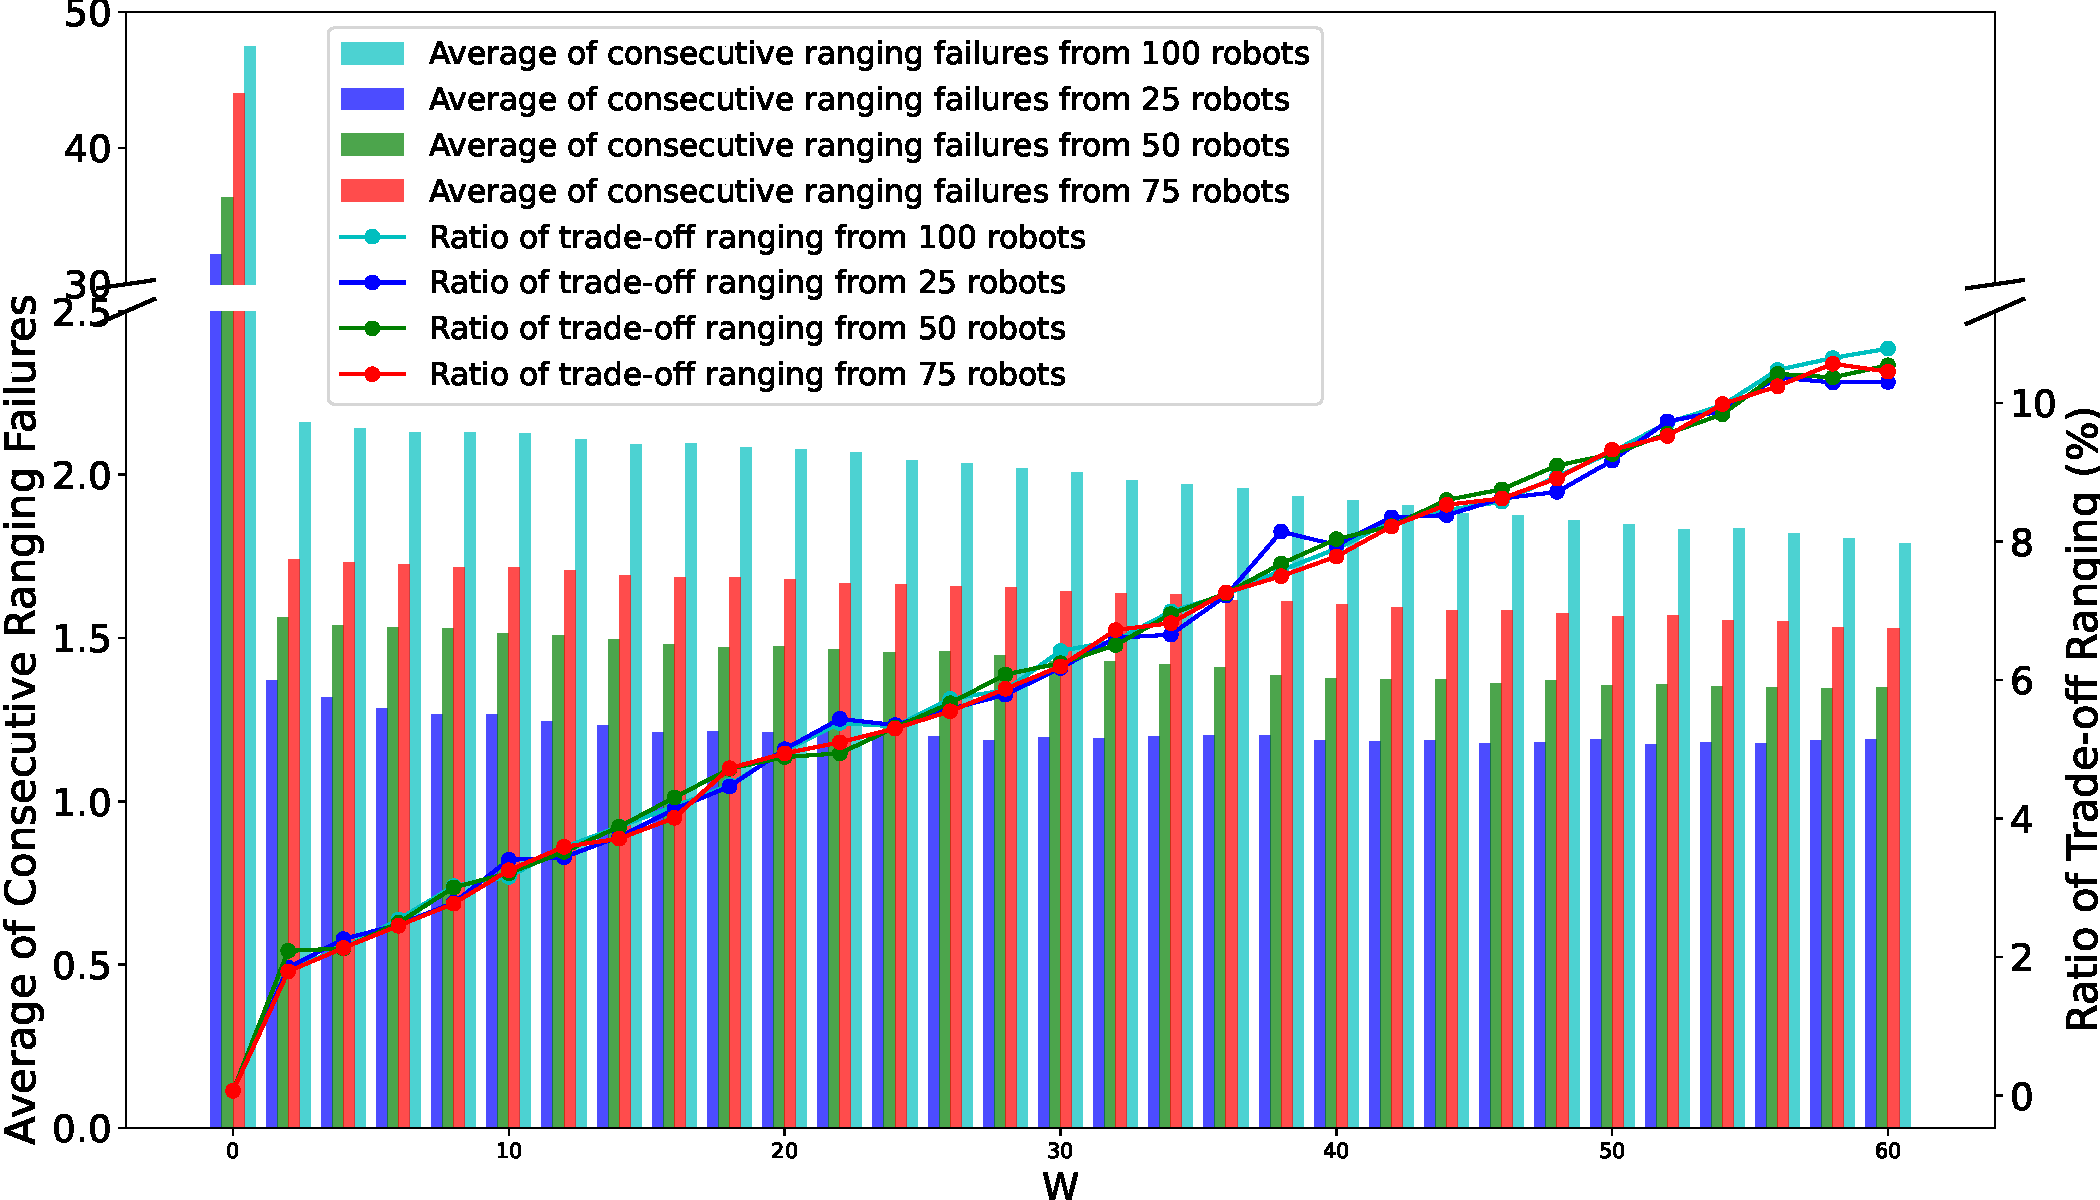
\includegraphics[width=0.8\textwidth]{figures/content/chapter3/robotsSimulation.pdf}}
\caption{
不同规模无人机集群在平均测距周期为100 ms、仿真时长为200s条件下的仿真结果
}
\label{fig:3_14}
\end{figure}
\subsection{真实世界中的鲁棒集群测距协议性能}
在本小节中，通过开展一系列大量真实世界中的无人机实验，对所提出测距协议的鲁棒性与准确性进行验证。

首先，在两台无人机执行测距的过程中，统计连续测距失败次数的平均值以及权衡测距的发生次数。
连续测距失败次数通过分析上一条成功接收报文的序列号进行计算；
权衡测距的概率则通过权衡测距发生次数与总测距次数之比进行统计。
在实验中，平均测距周期设置为 20 ms。
我们针对每一种不同的周期抖动取值，分别进行了 3 组实验，每组实验的测距持续时间为 120 s。
最终利用这些实验数据对相应的实验曲线进行拟合。

\begin{figure}[htbp]
  \centering
  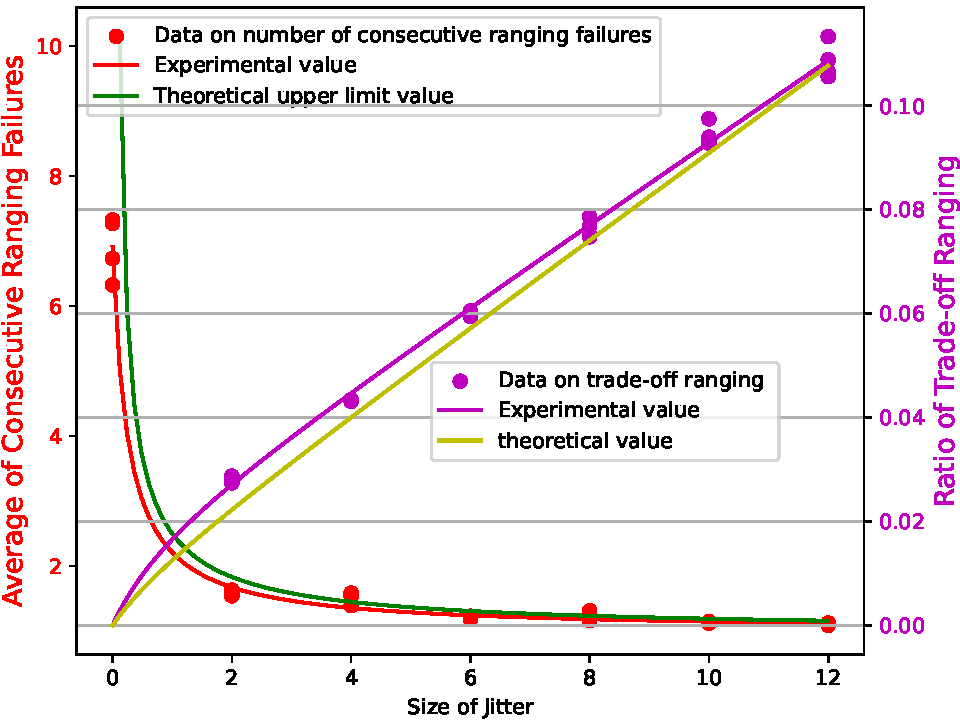
\includegraphics[width=.6\linewidth]{figures/content/chapter3/Comparison_TheoryandExperiment.pdf}
  \caption{鲁棒集群测距协议的理论分析与实验结果对比}
  \label{fig:3_15}
\end{figure}

如图\ref{fig:3_15}所示，实验结果与理论分析结果具有较高的一致性。
引入随机化周期后，连续测距失败的发生次数显著降低。
随着抖动幅度的增加，连续测距失败次数不再明显下降，而权衡测距发生的概率则持续快速上升。
真实实验结果验证了第\ref{sec:Theory}节中关于周期抖动对连续测距失败以及权衡测距概率影响的理论分析结论的正确性。

随后，我们在大规模无人机集群场景下对所提出的鲁棒集群测距协议的鲁棒性进行了系统评估。
通过逐步增大周期的抖动，观察连续测距失败次数的平均值、最大连续测距失败次数、权衡测距比例以及丢包率等指标的变化情况。
在实验设置中，共有 24 架无人机同时进行通信与测距，平均测距周期设置为 60 ms。
在 鲁棒集群测距协议运行过程中，对 120 s 内的数据进行了统计与分析。

\begin{figure}[htbp]
  \centering
  \includegraphics[width=.6\linewidth]{figures/content/chapter3/24RobotExpone.pdf}
  \caption{24 架无人机连续测距失败次数最大值与平均值的统计结果 }
  \label{fig:3_16}
\end{figure}

如图\ref{fig:3_16}所示，随着抖动幅度的增加，连续测距失败的平均值和最大值均呈现明显下降趋势。
在引入随机化周期后，这两个指标均出现显著降低，并且随着抖动值的进一步增大，其波动范围逐渐减小。
当抖动值大于 10 时，连续测距失败的最大值与平均值基本趋于稳定，不再发生明显变化。

\begin{table}[htbp]
\centering
\caption{24 架无人机实验中权衡测距比例与收包成功率统计结果}
\label{tab:jitter_results}

\resizebox{\textwidth}{!}{
\begin{tabular}{c|cccccccccc}
\hline
Jitter size & 0 & 2 & 4 & 6 & 8 & 10 & 14 & 20 & 30 & 40 \\
\hline
权衡测距比例
& 0.5\% & 0.7\% & 1.28\% & 1.86\% & 2.31\% & 3.58\% & 4.27\% & 6.34\% & 9.48\% & 12.3\% \\

收包成功率
& 85.49\% & 85.06\% & 85.13\% & 85.11\% & 85.04\% & 84.92\% & 85.24\% & 85.15\% & 84.96\% & 85.01\% \\
\hline
\end{tabular}
}

\end{table}

如表\ref{tab:jitter_results}所示，与第\ref{sec:Theory}节中的理论分析结果一致，权衡测距的比例随着抖动值的增大而逐渐上升。
同时，尽管测距周期引入了随机化，无人机集群的丢包率基本保持不变。
上述实验结果不仅验证了所提出协议在测距过程中能够有效缓解连续测距失败的问题，同时也为后续大规模实验中随机化周期参数的选择提供了重要参考。

\begin{figure}[htbp]
  \centering
  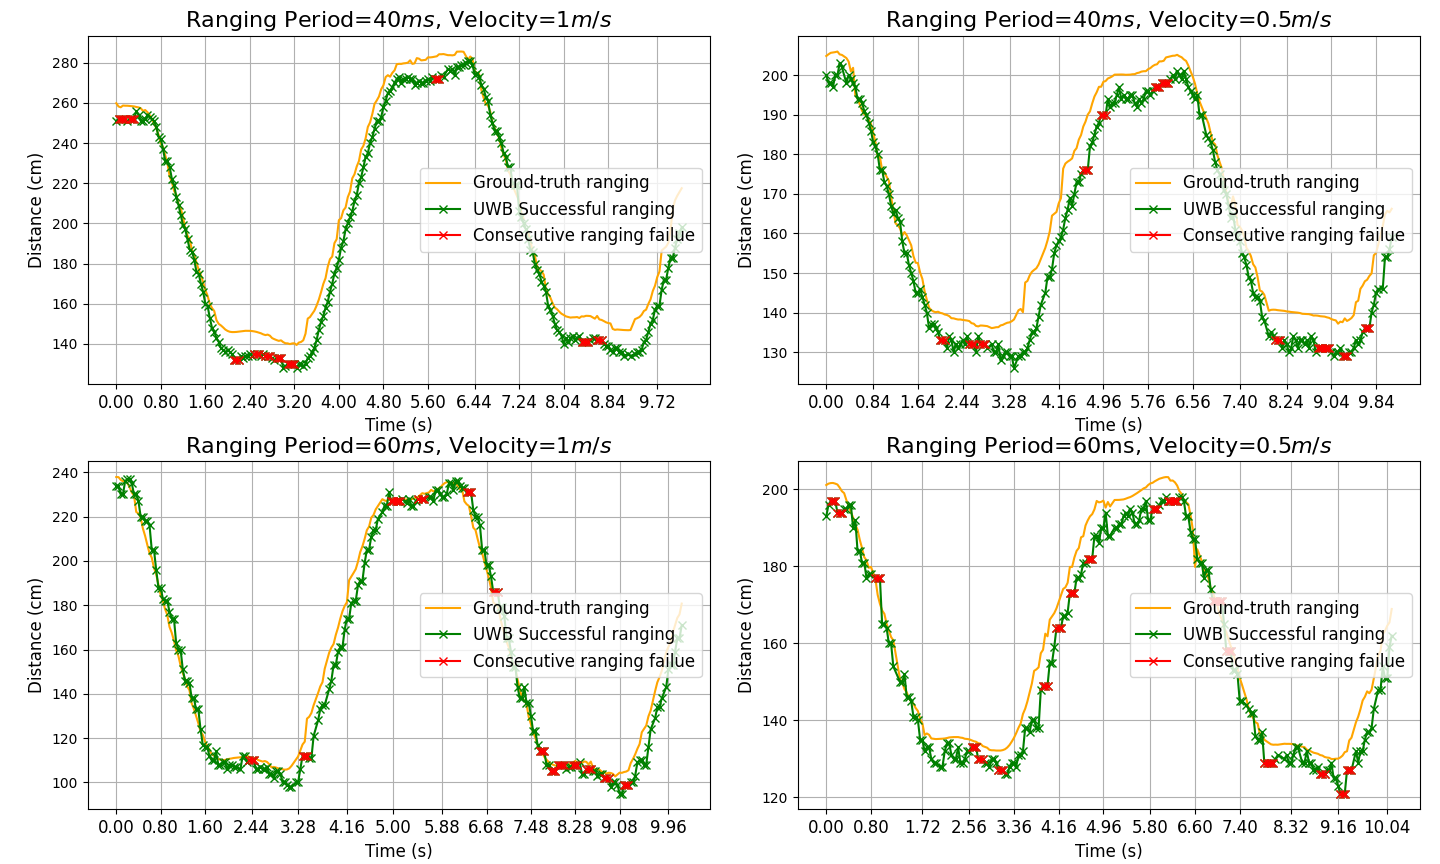
\includegraphics[width=.9\linewidth]{figures/content/chapter3/multiMeasurementsV2.png}
  \caption{应用鲁棒集群测距协议后，不同测距周期与速度下连续测距失败的缓解情况}
  \label{fig:3_17}
\end{figure}

最后，我们在图\ref{fig:3_16}所示的实验平台基础上，采用优化后的抖动参数设置的基础上，并在不同的运动速度和测距周期条件下进行了进一步实验。
实验结果如图\ref{fig:3_17}表明，在应用鲁棒集群测距协议后，与理论分析结果一致，测距失败在时间上呈现更加分散的分布特性，长时间连续测距失败现象不再出现。


\subsection{自适应协同定位算法性能}

为了评估所提出自适应协同定位算法的定位精度与稳定性，本文首先通过仿真实验对算法性能进行验证，并与传统扩展卡尔曼滤波方法进行对比分析。
实验主要关注在噪声统计特性未知或存在建模误差的情况下，算法对系统状态的估计能力。

在仿真中，系统采样周期设定为$\Delta t=0.1s$，每次实验包含 100 个时间步。为了保证实验结果的统计稳定性，每组实验进行 100 次 蒙特卡洛重复仿真，并对结果取平均值。
实验中一无人机静止，另一无人机以1 m/s 的速度匀速向前运动，其中过程噪声协方差矩阵$\Omega_{0} = =\operatorname{diag}(0.2^2,0.2^2,0.3^2,0.2^2,0.2^2, 0.3^2)$, 
量测噪声为高斯白噪声，其协方差设定为 $\Lambda_{0} = 0.1^2$​。
初始协方差矩阵设定为 $\Sigma_{ij,0} = =\operatorname{diag}(5,5,0.1)$

为了评估所提出算法的性能，本文选取以下两种方法进行对比：第一种传统扩展卡尔曼滤波
采用标准扩展卡尔曼滤波进行状态估计，量测噪声协方差在整个滤波过程中保持固定。
第二种为本文提出的自适应扩展卡尔曼滤波，在每个时刻通过迭代更新状态估计、协方差矩阵以及量测噪声协方差，实现对系统不确定性的自适应估计。
为了研究迭代次数对算法性能的影响，本文分别设置迭代次数 $N=1,2,3,4,5$。

本文采用位置均方根误差（Root Mean Square Error，RMSE）作为算法性能评价指标：
\begin{equation}
R M S E=\sqrt{\frac{1}{T} \sum_{k=1}^{T}\left\|\hat{p}_{k}-p_{k}\right\|^{2}}
\end{equation}
其中：$p_{k}$  为真实位置,$\hat{p}_{k}$  为估计位置, $T$  为仿真步数.

\begin{figure}[htbp]
  \centering
  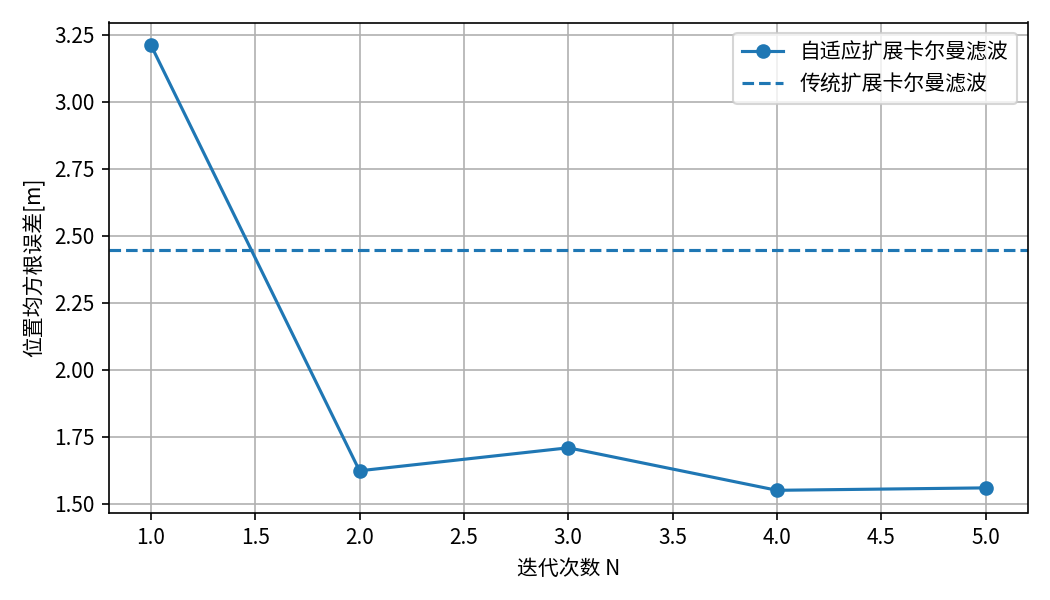
\includegraphics[width=.7\linewidth]{figures/content/chapter3/AEKF.png}
  \caption{自适应EKF与传统EKF定位误差对比图}
  \label{fig:3_19}
\end{figure}

从实验结果图\ref{fig:3_19}中可以看出，不同迭代次数下算法的定位误差均方根变化情况，并与传统扩展卡尔曼滤波的定位误差进行了对比。
图中横轴表示迭代次数 N，纵轴表示位置估计误差的均方根值，虚线表示传统 EKF 算法的定位误差水平。

当迭代次数 N = 1 时，算法的 RMSE 约为 3.2 m，此时误差较大，说明在未进行充分迭代优化的情况下，状态估计精度仍然较低。
随着迭代次数增加，定位误差明显下降。当 N = 2 时，RMSE 降至约 1.62 m，相较于传统 EKF 的约 2.45 m，定位精度得到明显提升。
当迭代次数继续增加时，RMSE 的变化逐渐趋于稳定。
结果表明，当迭代次数达到 4 次左右时，算法的估计精度已经基本收敛，继续增加迭代次数对精度提升的作用较为有限。

与传统 EKF 算法相比，所提出的迭代算法在 N ≥ 2 时均表现出更低的定位误差，RMSE 从 EKF 的约 2.45 m 降低到约 1.55 m，误差降低约 36\%。

综上所述，仿真结果验证了所提出算法在定位精度方面相较于传统 EKF 具有明显优势，并且在迭代次数达到一定程度后能够快速收敛，在保证定位精度的同时兼顾计算效率。

\begin{figure}[htbp]
  \centering
  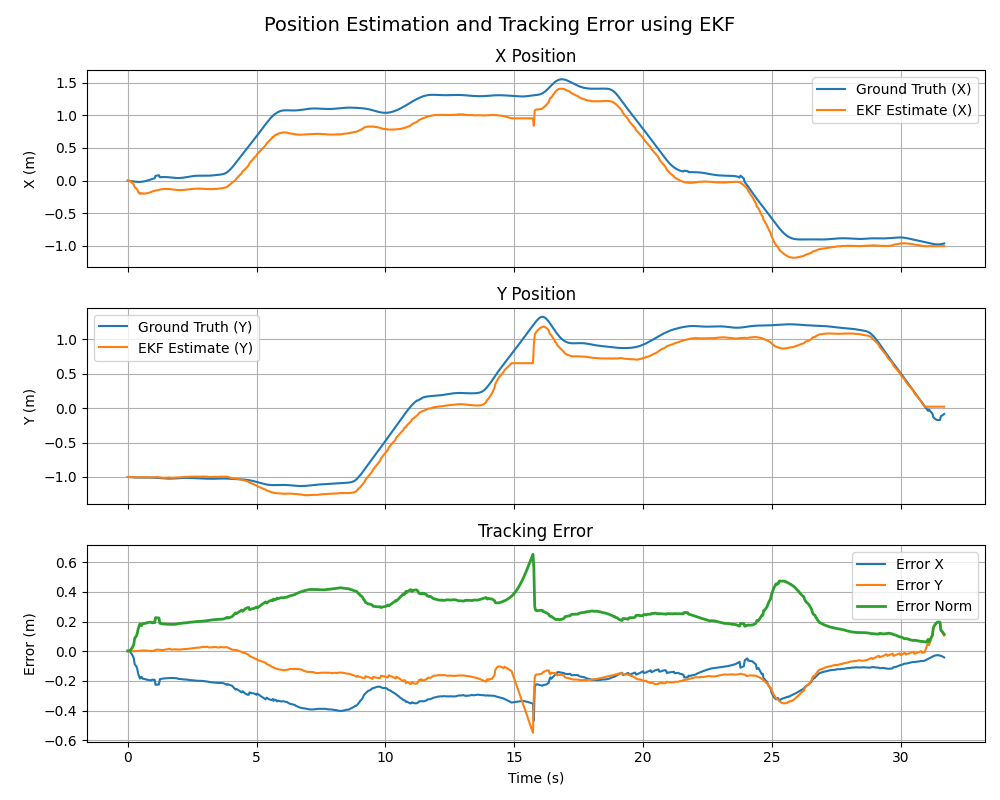
\includegraphics[width=.6\linewidth]{figures/content/chapter3/EKFError.png}
  \caption{传统EKF定位误差图}
  \label{fig:3_20}
\end{figure}
为验证所提出自适应扩展卡尔曼滤波算法在无人机相对定位中的性能，本文设计并开展了双无人机相对定位实验。
在实验场景中，选取两架无人机，其中一架无人机保持悬停状态，作为参考节点；
另一架无人机执行预设轨迹飞行，其运动轨迹为边长为 1m×1m 的正方形路径。
该实验设计能够构建具有代表性的动态相对运动场景，有利于评估定位算法在实际飞行过程中的跟踪性能与稳定性。

在测量方面，系统采用超宽带模块进行相对距离观测，测距平均周期约为60 ms。基于前文的鲁棒集群测距协议，在测距周期中引入幅值为6ms的随机扰动，使得测距的结果更为鲁棒。
同时，在滤波过程中，AEKF算法基于上述仿真实验的分析在每一时刻执行3次迭代更新，以增强对非线性系统的逼近能力，提高状态估计精度。

实验过程中，通过Vicon光学运动捕捉系统获取高精度位置数据，作为真实值（Ground Truth）。
将滤波器输出的估计位置与真实值进行对比，从而计算定位误差并评估算法性能。


\begin{table}[htbp]
\centering
\caption{两种算法定位误差统计对比}
\label{tab:error_comparison}
\begin{tabular}{lccc}
\toprule
算法类型 & X 轴 (m) & Y 轴 (m) & 总误差 (m) \\
\midrule
传统 EKF & 0.3896 & 0.2715 & 0.4749 \\
自适应 AEKF & \textbf{0.1651} & \textbf{0.1868} & \textbf{0.2493} \\
\bottomrule
\end{tabular}
\end{table}



实验分别运行基于传统扩展卡尔曼滤波（EKF）和自适应扩展卡尔曼滤波（AEKF）的定位计算，记录目标无人机在 $X$ 轴与 $Y$ 轴方向的实时位置误差。
具体的误差统计数据如表\ref{tab:error_comparison}所示。



AEKF 算法的总均方根误差（RMSE）为 0.2493 m，相较于传统 EKF 算法的 0.4749 m，定位精度提升了约 47.5\%。
\begin{figure}[htbp]
  \centering
  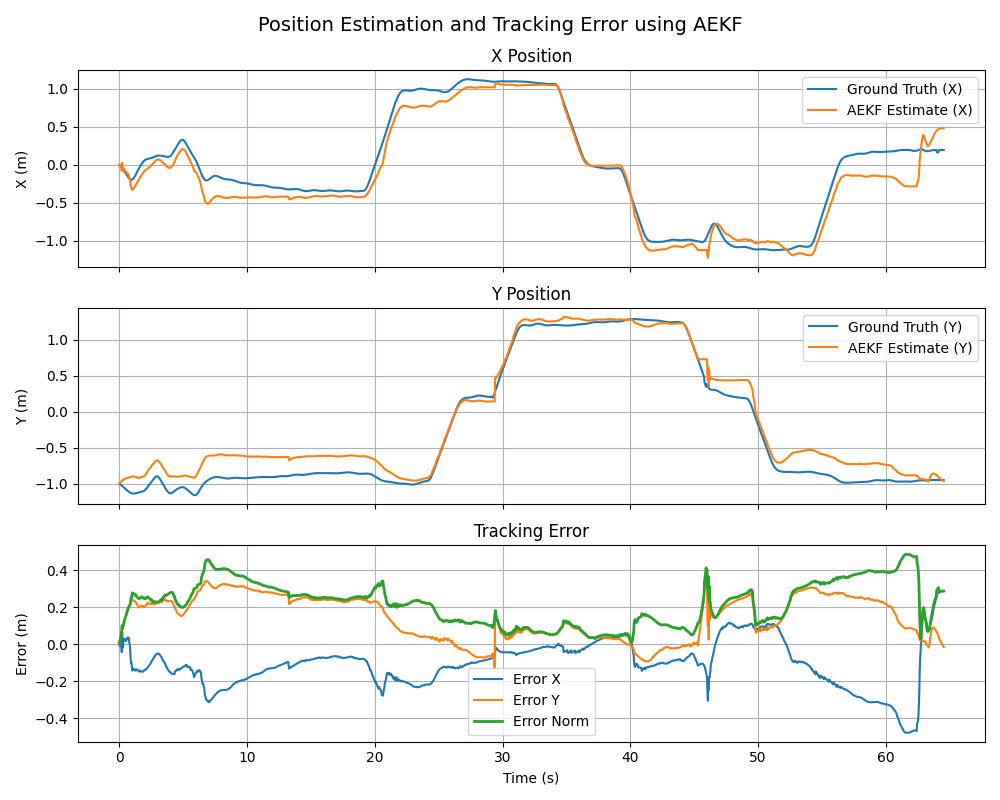
\includegraphics[width=.6\linewidth]{figures/content/chapter3/AEKFError.png}
  \caption{自适应EKF定位误差图}
  \label{fig:3_21}
\end{figure}
图 \ref{fig:3_20} 与图 \ref{fig:3_21} 分别展示了传统扩展卡尔曼滤波（EKF）与自适应扩展卡尔曼滤波（AEKF）在双机协同定位实验中的位置估计与跟踪误差时域曲线。
各子图中，蓝色曲线表示地面真实轨迹，橙色曲线表示滤波估计轨迹；
底部误差子图中，蓝色、橙色与绿色曲线分别对应 X 轴误差、Y 轴误差及总误差范。

对比两图的上部位置跟踪曲线可以观察到：传统 EKF：在目标无人机执行 1 m × 1 m 正方形轨迹的转弯机动阶段（约 $t = 2.5$ s、$5.0$ s、$7.5$ s 等时刻），估计轨迹与真实轨迹之间存在肉眼可辨的滞后与超调现象。尤其在 Y 轴方向，当无人机由上升段转入平飞段时，EKF 估计值未能及时响应运动状态的变化，导致橙色曲线明显偏离蓝色真实值。
自适应 AEKF：在全飞行时段内，橙色估计曲线与蓝色真实曲线几乎紧密贴合。即便在正方形四个顶点的急转弯处，AEKF 仍能保持对真实轨迹的高保真跟踪，未见明显的滞后或过冲。这表明自适应协方差调整机制能够实时感知机动状态的变化，并动态增强滤波器对观测新息的响应能力。

上述实验结果表明，所采用的自适应 EKF 算法在仅增加少量计算迭代次数的前提下，能够有效克服传统 EKF 在动态环境及测距抖动下的精度发散问题。
该算法在保证厘米级定位精度的同时，为后续的大规模集群编队飞行提供了可靠的相对定位数据支撑。
\subsection{  大型集群编队飞行实验}

本小节展示了一项真实飞行实验，用于验证领导-跟随编队控制的效果。
实验中基于上文的自适应协同定位算法实现无人机之间的相对定位。
实验共使用13架Crazyflie无人机，初始时各无人机间距为1米。
在飞行过程中，9架无人机在边长为2 m的内环区域飞行，其余4架无人机在边长为4 m的外环区域飞行。
平均测距周期为60 ms，抖动设置为6。
飞行过程如图\ref{fig:3_22}所示，四张图分别展示了无人机的初始位置、跟随阶段以及编队变化阶段。
红色圆圈表示领航无人机，其他颜色圆圈表示跟随无人机。

\begin{figure}[htbp]
  \centering
  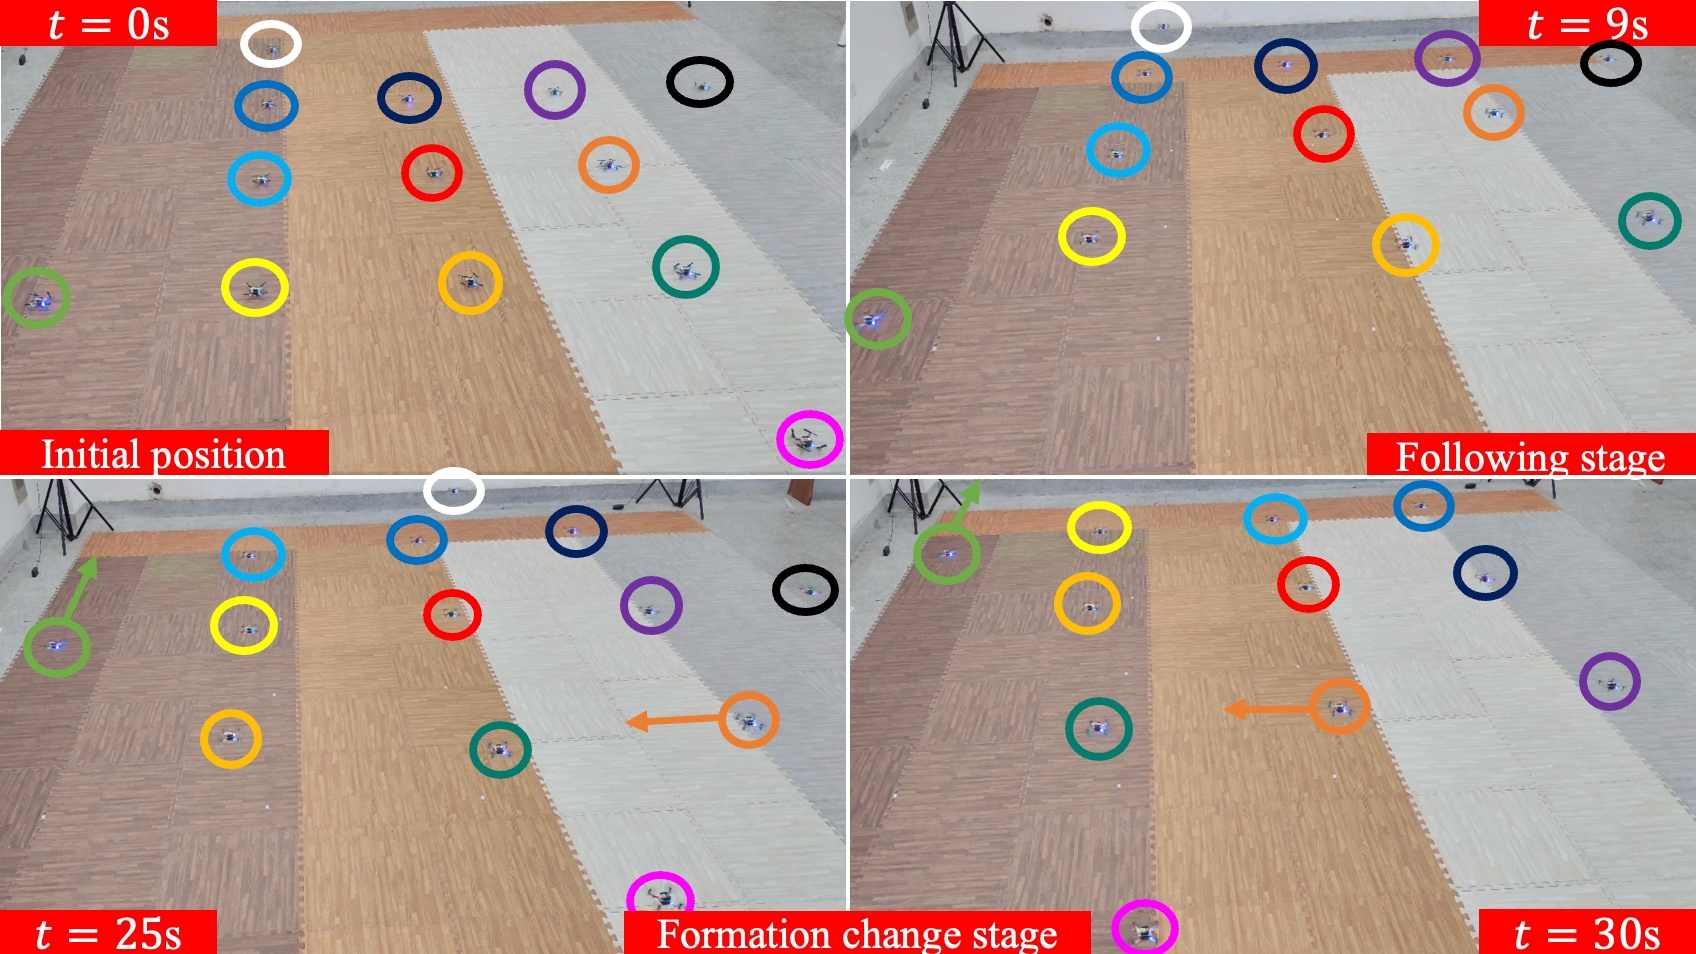
\includegraphics[width=.7\linewidth]{figures/content/chapter3/uwb_13_formation.png}
  \caption{13架无人机编队飞行的顶部视图}
  \label{fig:3_22}
\end{figure}

在 t= 0 s时，所有无人机从各自已知的初始位置起飞；
经过5秒后，无人机已形成编队，并保持与红色圆圈编号为1的无人机的相对位置，该无人机以随机方式飞行。
从 t= 15 s开始，所有无人机开始改变编队，图中箭头表示下一步编队变化的方向。
此外，在编队飞行过程中，记录了4架无人机相对于橙色圆圈（编号为2的无人机）的UWB测距数据及地面真实距离，如图\ref{fig:3_23}(a)所示。
图\ref{fig:3_23}显示了测距误差分布，两架无人机之间距离测量的平均绝对误差约为6.21 cm。

\begin{figure}[ht]
    \centering
    
    \begin{minipage}[b]{0.5\textwidth}
        \centering
        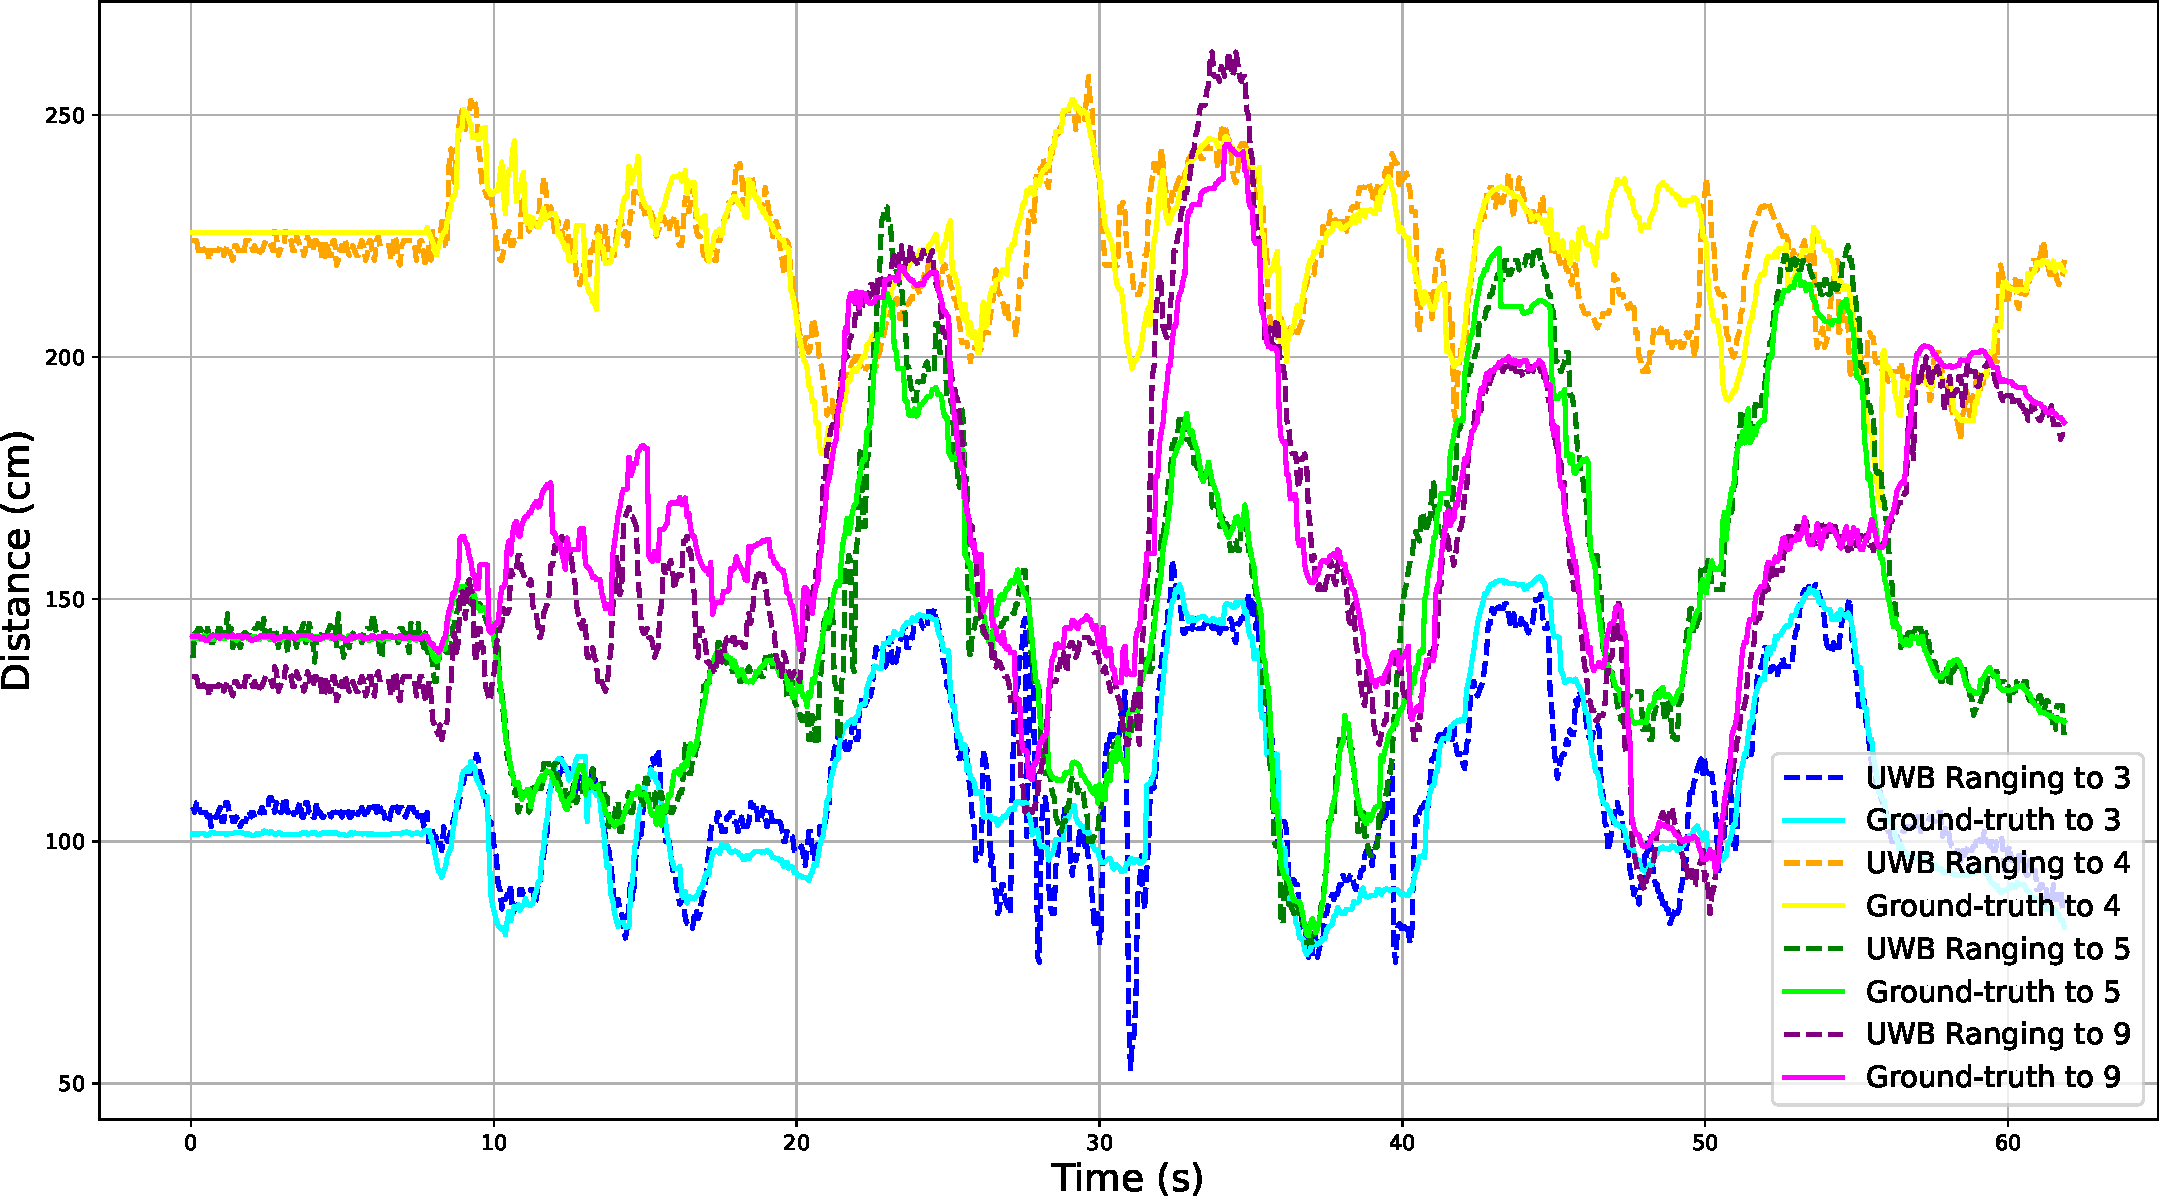
\includegraphics[width=\textwidth, trim={0cm 0cm 0cm 0cm}, clip]{figures/content/chapter3/uwb_4_distance.pdf}
        \\(a) UWB测距结果
    \end{minipage}
    \begin{minipage}[b]{0.3\textwidth}
        \centering
        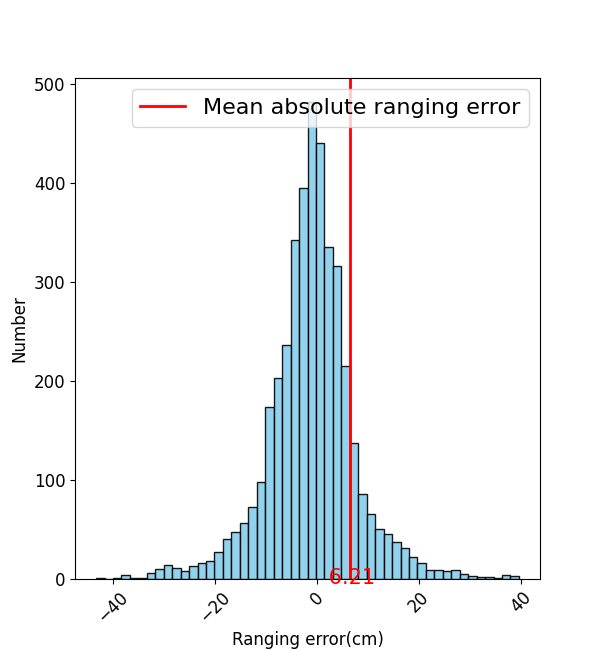
\includegraphics[width=\textwidth, trim={0.2cm 0cm 0cm 0.3cm}, clip]{figures/content/chapter3/errorDistribution.png}
        \\(b) 测距误差分布
    \end{minipage}
    \caption{13架无人机编队飞行过程中获取的5架无人机测量数据}
    \label{fig:3_23}
\end{figure}

实验结果表明，所提出的无人机集群自适应协同定位算法在动态且密集的大规模无人机群中，能够实现稳健且精确的距离测量。
因此，该算法可为大规模无人机群的高效定位和自主编队飞行任务提供可靠支持。

\section{本章小节}

本章针对无人机集群相对定位问题，提出了一种基于 UWB 的自适应协同定位方法。
首先，为解决大规模集群中测距冲突和连续测距失败的问题，设计了一种鲁棒集群测距协议，并通过引入周期抖动机制以及权衡测距方法，提高了测距成功率和系统稳定性。
随后，在扩展卡尔曼滤波框架下引入期望最大化算法，实现对系统噪声参数的在线估计，从而提升无人机协同定位的精度与鲁棒性。
通过仿真实验和真实无人机编队飞行实验对所提出方法进行了验证，实验结果表明该方法能够在多无人机动态环境中实现稳定且高精度的相对定位。

      % 第三章：
\chapter{无人机风险感知的自主航方法}


\section{引言}
无人机自主导航能力是保障无人机在复杂环境中安全、高效执行任务的重要基础。
然而，在复杂未知环境中实现安全可靠的自主导航与避障仍然是无人机研究中的关键问题。
传统基于规则或模型的方法在结构化环境中能够取得一定效果，但在动态变化和部分可观测环境下，其适应能力和鲁棒性仍然有限。
因此，近年来深度强化学习被广泛应用于无人机自主导航任务中，通过与环境交互不断学习策略，以最大化长期累积回报。

尽管深度强化学习在路径规划和决策控制方面表现出较强的能力，但其核心优化目标通常是最大化期望累积回报，这往往隐含地假设未来回报分布相对稳定，并未充分考虑低概率但高风险的灾难性事件。
在无人机导航避障任务中，这类事件可能包括突发障碍物、飞行姿态异常以及极端环境干扰等。
由于这些事件在训练过程中出现频率较低，在传统强化学习的回报计算中所占权重有限，模型往往难以学习到针对这些风险场景的有效策略。
然而，对于安全关键系统而言，一次灾难性事件就可能导致任务失败甚至设备损毁，因此仅依赖期望回报最大化的策略难以满足无人机导航系统对安全性的要求。

另一方面，无人机在实际飞行过程中需要对环境变化做出快速响应。
虽然边缘计算技术可以通过将部分计算任务卸载至网络边缘服务器来提升整体计算能力，但在无人机导航避障任务中，依赖远程推理往往会受到网络延迟、数据传输时间以及通信带宽限制等因素的影响。
对于需要毫秒级响应的飞行决策而言，这种延迟可能导致无人机无法及时做出避障动作，从而增加发生碰撞或任务失败的风险。
因此，在无人机自主导航系统中，如何在有限计算资源条件下实现高效、可靠且实时的决策策略，是一个亟需解决的重要问题。

针对上述问题，本文提出了一种面向无人机自主导航任务的风险感知强化学习方法，在复杂未知环境中实现安全高效的自主避障与导航决策。
该方法通过对强化学习回报分布进行建模，引入风险评估机制，使无人机在决策过程中能够同时考虑任务收益与潜在风险，从而在保证导航效率的同时降低灾难性事件发生的概率。
此外，为满足无人机实时决策的需求，本文对训练后的强化学习模型进行了量化与压缩，使其能够在资源受限的嵌入式平台上实现高效推理与导航。
最终，所提出的方法在Crazyflie 2.1 Brushless微型四旋翼无人机平台上完成了实际部署，并通过仿真与真实飞行实验验证了算法在复杂环境中的有效性与鲁棒性。
\section{基于分布式强化学习的导航模型构建与训练}

\subsection{问题定义与奖励函数设计}
\label{sec:stateDefine}
本文将无人机导航任务建模为部分可观测马尔可夫决策过程（Partially Observable Markov Decision Process，POMDP）\cite{arcieri2025deep}。
在POMDP建模中，其通常被表示为一个五元组$(S, A, O, P, R, \gamma)$。
其中，$S$、$A$和$O$分别表示状态空间、动作空间以及观测空间。
无人机在离散时间步下与环境进行交互。
在每一个时间步$t$，无人机从环境中获得观测信息$o_{t} \in O$，并根据策略函数$\pi\left(a_{t} \mid o_{t}\right)$选择动作$a_{t} \in A$。
执行该动作后，系统状态由$s_{t}$按照状态转移概率$P\left(\cdot \mid s_{t}, a_{t}\right)$转移至下一状态$s_{t+1}$，同时环境产生即时奖励$r_{t}=R\left(s_{t}, a_{t}\right)$，并生成新的观测$o_{t+1} \sim O\left(\cdot \mid s_{t+1}, a_{t}\right)$。
在给定策略$\pi$的情况下，未来累积折扣回报可以表示为随机变量
$Z^{\pi}\left(s_{t}, a_{t}\right)=\sum_{k=0}^{\infty} \gamma^{k} R\left(s_{t+k}, a_{t+k}\right)$。
其中,$\gamma \in(0,1)$为折扣因子，用于衡量未来奖励的重要程度。传统强化学习方法通常以最大化该随机回报的期望值为目标，即动作价值函数
$Q^{\pi}\left(s_{t}, a_{t}\right)=\mathbb{E}\left[Z^{\pi}\left(s_{t}, a_{t}\right)\right]$。

\begin{figure}[htbp]
  \centering
  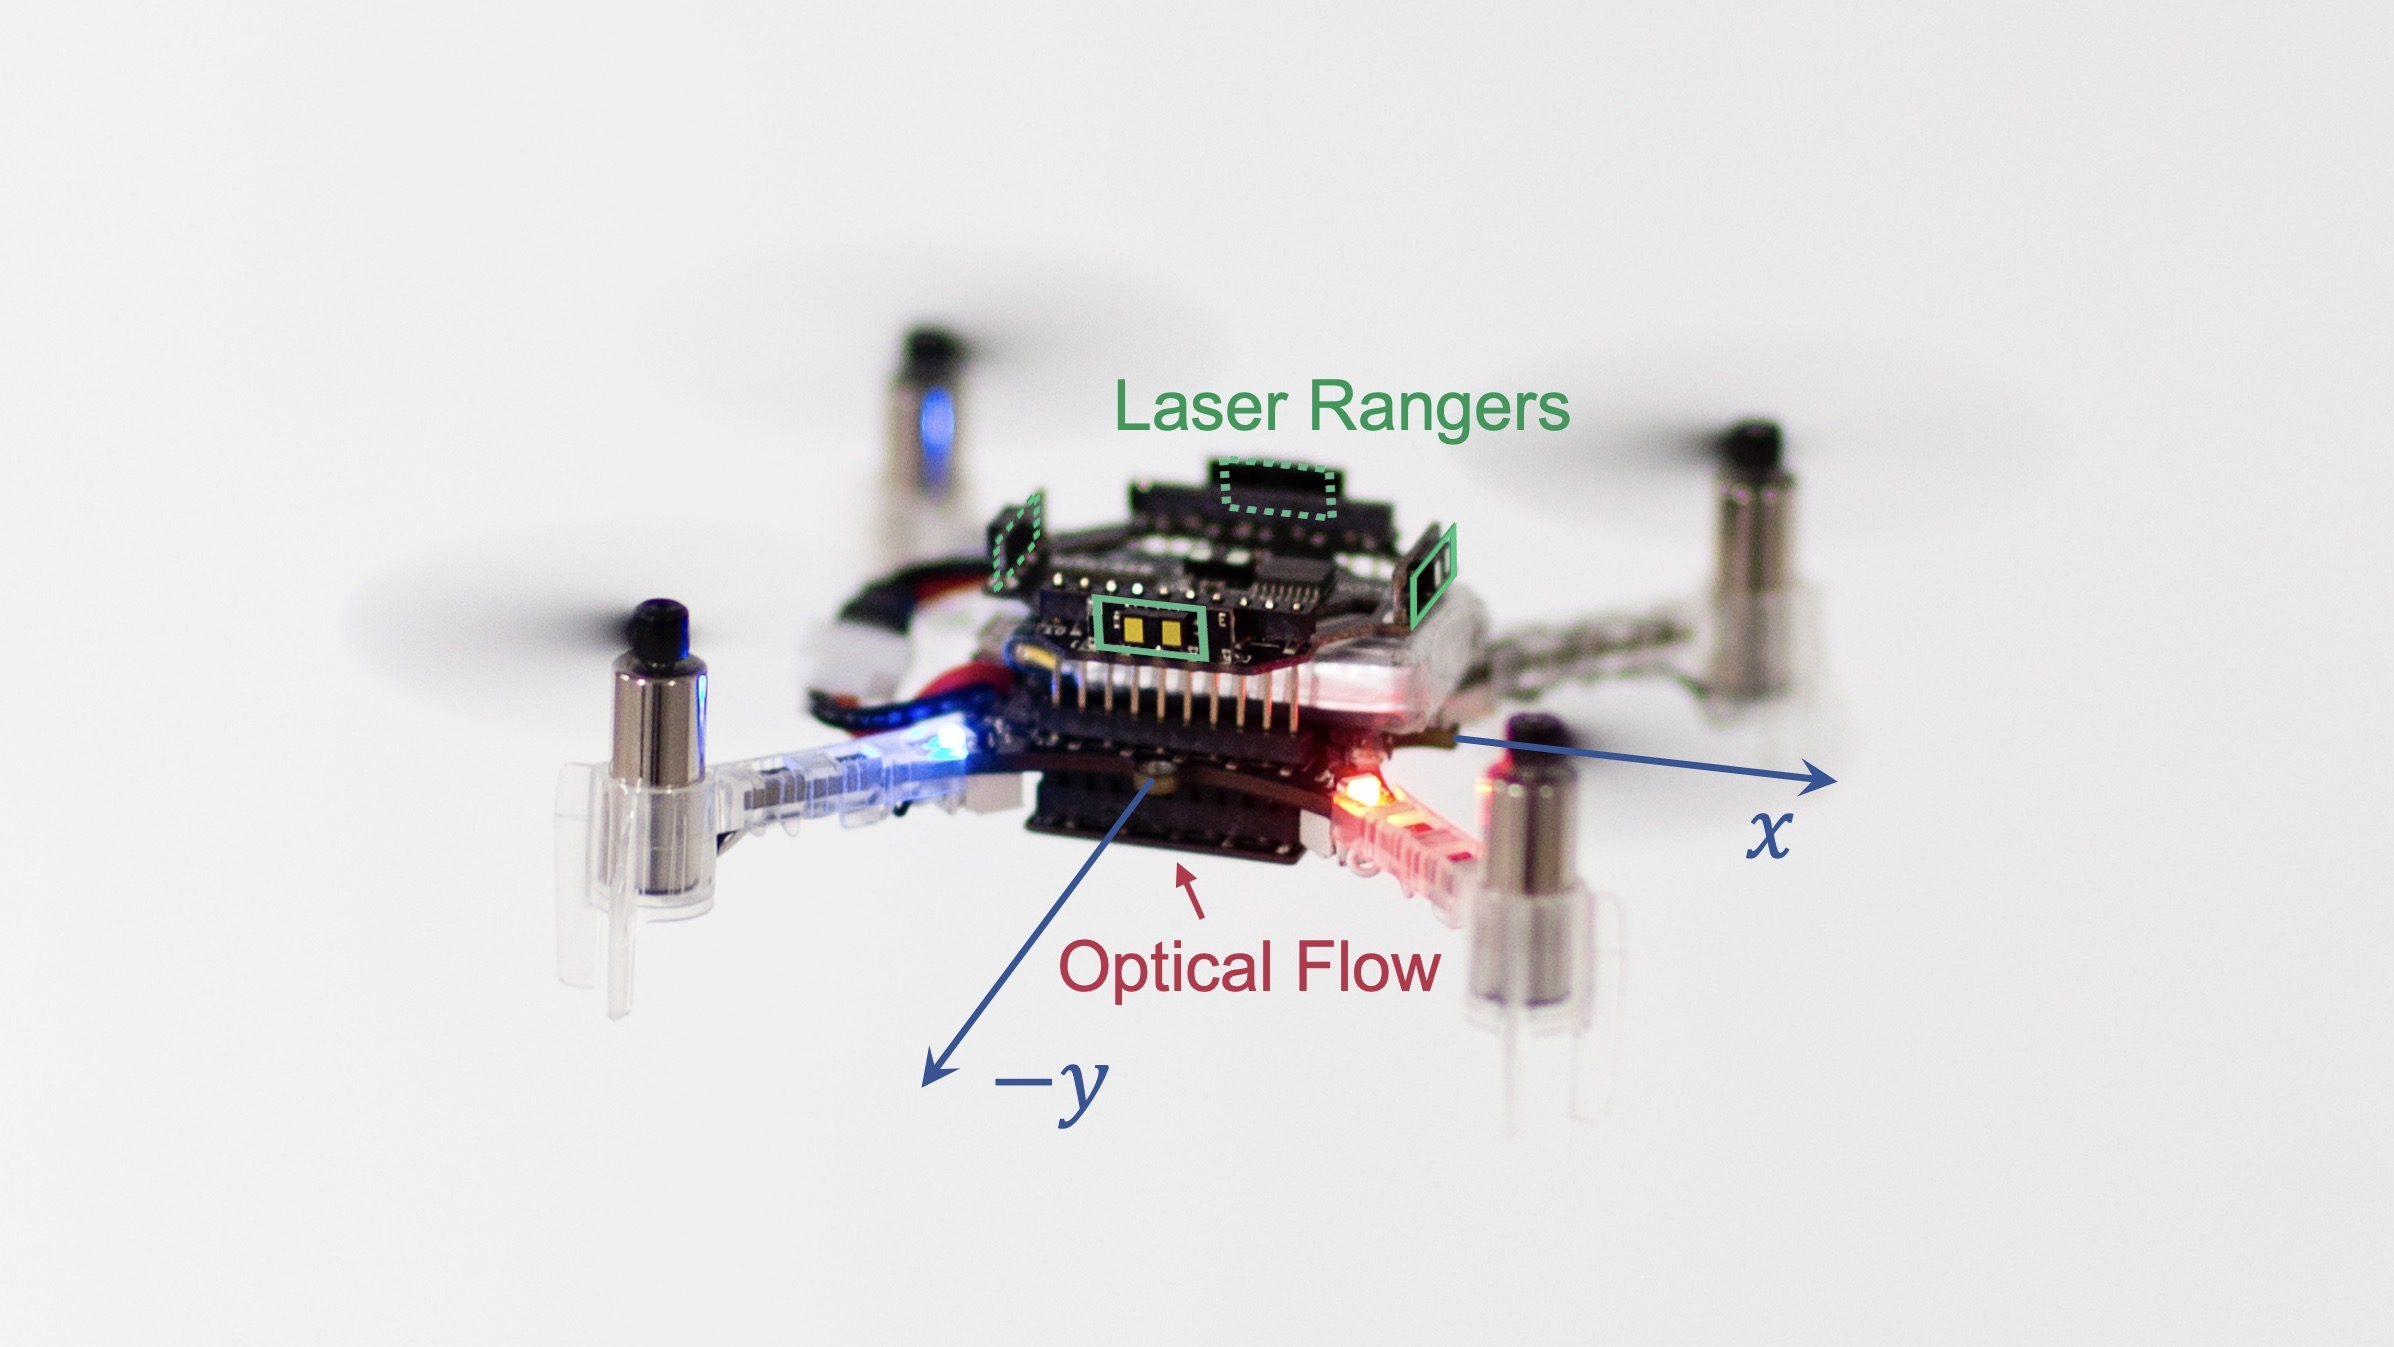
\includegraphics[width=.6\linewidth]{figures/content/chapter4/crazyflie.jpeg}
  \caption{带有4个激光器的微型无人机设备，用于探测障碍物}
  \label{fig:4_1}
\end{figure}

无人机的状态与观测部分中，本文选用Crazyflie 2.1 Brushless纳米四旋翼无人机作为实验平台。
如图\ref{fig:4_1}所示，该无人机在机体$x$轴和$y$轴的正负方向上分别安装了四个激光测距传感器，用于检测周围障碍物。
同时，无人机还配备了光流相机扩展版，用于估计飞行速度，从而实现底层飞行控制。
在导航任务中，系统状态空间$S$包含无人机自身状态、目标位置以及环境障碍物信息。
状态可以表示为
$s_{t}=\left\langle p, d_{g}, d_{o}\right\rangle$。
其中， $p$  表示无人机的全局位置；
$d_{g}=\left\|p-p_{g}\right\|_{2}$  表示无人机与目标点之间的欧氏距离；
$d_{o}$  为一个向量，用于表示无人机到周围障碍物的距离信息。
由于机载传感器数量和测量能力有限，无人机无法完全观测到完整的系统状态。
因此，在实际决策过程中，无人机仅能够获得部分观测信息。观测向量表示为
$o_{t}=\left\langle p, d_{g}, d_{l}\right\rangle$。
其中，$d_{l}$表示激光测距传感器的反射距离。
激光传感器的最大探测距离为4 m。
在真实飞行实验中，无人机的全局位置$p$以及目标距离$d_{g}$由外部运动捕捉系统提供。

为了适配所提出的算法，本文将动作空间$A$设计为离散化的速度控制指令，包括不同大小和方向的速度组合。
速度幅值被离散为$m$个指数间隔分布在区间$\left(0, v_{m}\right]$内的取值，其中$v_{m}$表示无人机允许的最大飞行速度。
由于激光传感器只能检测与激光束方向相交的障碍物，因此无人机的运动方向被离散为在区间 $[0,2 \pi)$内均匀分布的4个方向。

奖励函数通过人工设计，用于鼓励无人机尽快到达目标点，同时对发生碰撞或接近障碍物的行为进行惩罚。奖励函数定义为
\begin{equation}
  R\left(s_{t}, a_{t}\right)=\left\{\begin{array}{ll}
50, & d_{g}<d_{f} \\
5\left(d_{o}-d_{s}\right), & r_{d}<d_{o}<d_{s} \\
-25, & d_{o}<r_{d} \\
-0.1, & \text { otherwise }
\end{array}\right.
\end{equation}
其中，$d_{f}$表示到达目标点的判定阈值；$d_{o}$表示无人机到最近障碍物的距离；$d_{s}$表示安全距离阈值；$r_{d}$表示无人机机体半径。
通过上述奖励设计，可以引导无人机在保持安全距离的前提下快速到达目标位置，从而实现安全高效的自主导航。
\subsection{自适应风险倾向隐式分位数网络} 

为了能够在决策过程中动态调整策略的风险倾向，本文提出一种自适应风险倾向隐式分位网络（Adaptive Risk-Tendency Implicit Quantile Network，ART-IQN）算法。
该方法在分布式强化学习框架下构建，图\ref{fig:4_2}给出了 ART-IQN 的整体结构，其核心组成部分包括：
1）风险敏感隐式分位网络；
2）内在不确定性估计机制；
3）基于指数加权平均预测的不确定性预测方法，下文将分别对他们进行详细的阐述与说明。

\begin{figure}[htbp]
  \centering
  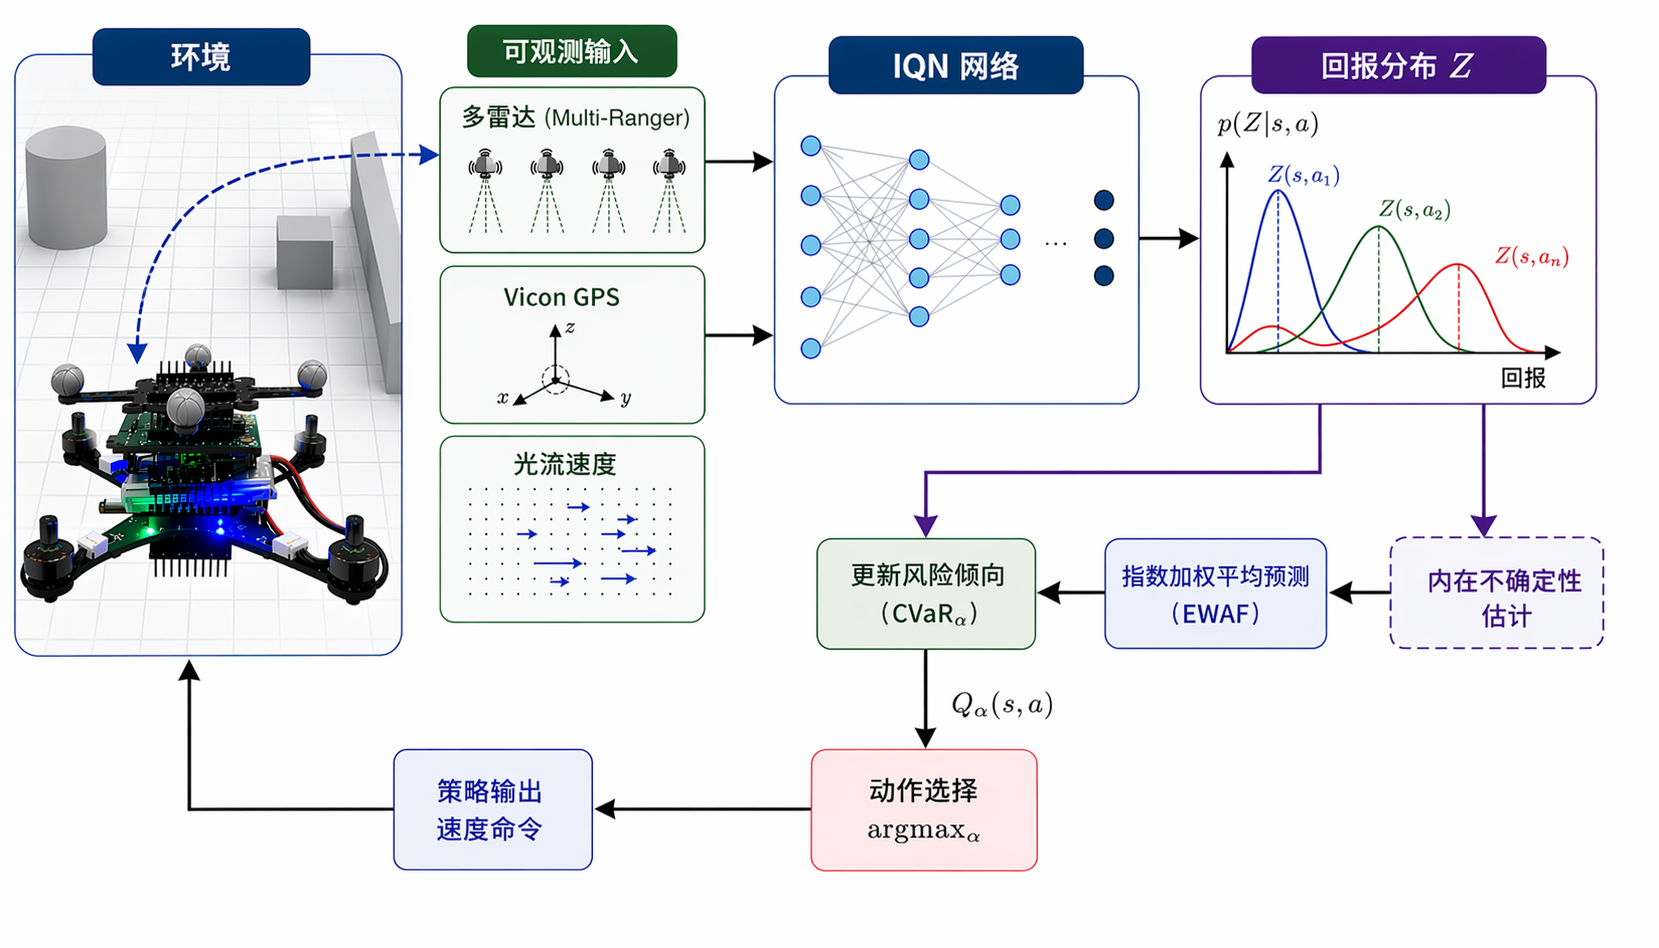
\includegraphics[width=.8\linewidth]{figures/content/chapter4/IQN.png}
  \caption{自适应风险倾向隐式分位网络框架}
  \label{fig:4_2}
\end{figure}

在分布式强化学习中，贝尔曼方程可以表示为
\begin{equation}
Z^{\pi}(s, a) \stackrel{D}{=} R(s, a)+\gamma Z^{\pi}\left(s^{\prime}, a^{\prime}\right)
\end{equation}
其中，符号$\stackrel{D}{=}$表示两个随机变量在分布意义下相等。
状态$s^{\prime}$和动作$a^{\prime}$的分布满足$s^{\prime} \sim P(s, a), a^{\prime} \sim \pi\left(\cdot \mid s^{\prime}\right)$。


在隐式分位数网络\cite{mokhtari2018iqn}方法中，我们使回报分布$Z^{\pi}(s, a$)通过其分位函数进行隐式表示，这种表示方式便于与不同风险度量方法结合，从而实现策略风险倾向的动态调整。
具体而言，分位函数由参数为$\theta$的神经网络进行近似表示：$Z_{\theta}^{\pi}(s, a ; \tau)$，
其中，$\tau \in[0,1]$表示分位水平。
为了训练该网络并优化参数$\theta$，需要进行分位回归\cite{buchinsky1998recent}，并采用Quantile Huber损失作为Wasserstein\cite{mokhtari2018iqn}距离的近似优化目标。

对于样本$\left(s, a, r, s^{\prime}\right)$，本文使用参数为$\theta^{\prime}$的神经网络对目标回报分布进行近似表示，并通过时间差分（Temporal Difference，TD）更新计算其误差。
其时序差分误差可表示为
\begin{equation}
\delta_{\tau, \tau^{\prime}}=r+\gamma Z_{\theta}^{\pi}\left(s^{\prime}, a^{\prime} ; \tau^{\prime}\right)-Z_{\theta}^{\pi}(s, a ; \tau)
\end{equation}
其中，$\tau$与$\tau^{\prime}$独立地从均匀分布中采样，即$\tau, \tau^{\prime} \sim U[0,1]$。

对应的$\tau$－分位Huber损失定义为
\begin{equation}
\begin{array}{l}
\rho_{\kappa}(\delta ; \tau)=|\tau-\mathbb{I}\{\delta<0\}| \frac{\mathcal{L}_{\kappa}(\delta)}{\kappa}, \text { with } \\
\mathcal{L}_{\kappa}(\delta)=\left\{\begin{array}{ll}
\frac{1}{2} \delta^{2} & \text { if }|\delta| \leq \kappa \\
\kappa\left(|\delta|-\frac{1}{2} \kappa\right) & \text { otherwise }
\end{array}\right.
\end{array}
\label{equ:Huber}
\end{equation}
其中, $\mathbb{I}$为指示函数，参数$\kappa$用于实现平滑梯度裁剪。
在实际训练中，通过采样$N$个分位值$\tau$以及$N^{\prime}$个目标分位值$\tau^{\prime}$，最终得到网络参数$\theta$的优化目标：
\begin{equation}
\mathcal{L}(\theta)=\frac{1}{N \cdot N^{\prime}} \sum_{i=1}^{N} \sum_{j=1}^{N^{\prime}} \rho_{\kappa}\left(\delta_{\tau_{i}, \tau_{j}^{\prime}} ; \tau_{i}\right)
\label{equ:lossfunction}
\end{equation}
通过对该损失函数进行反向传播优化，可以最小化当前回报分布$Z^{\pi}(s, a)$与目标分布$R(s, a)+\gamma Z^{\pi}\left(s^{\prime}, a^{\prime}\right)$之间的Wasserstein距离。

在风险敏感策略与风险度量方面，分布式强化学习通过对回报分布进行建模，使策略能够结合不同的风险度量指标进行决策。
通常情况下，可以通过扭曲期望来构造风险敏感策略。
该期望是在回报分布上施加一个单调非减的扭曲函数$\beta:[0,1] \rightarrow[0,1]$，并满足$\beta(0)=0, \beta(1)=1$。
在该扭曲函数作用下，回报分布的扭曲期望定义为$Q_{\beta}=\int_{0}^{1} F_{Z}^{-1}(\tau) d \beta(\tau)$。
其中，$F_{Z}^{-1}(\tau)$表示回报分布的分位函数。
实际上，该期望可以通过对分位值进行加权求和来近似计算。
具体而言，通过从均匀分布中采样$K$个分位值$\tilde{\tau}\sim U[0,1]$来近似$Q_{\beta}$，可得到基于样本的风险敏感策略：
\begin{equation}
\pi_{\beta}(s)=\arg \max _{a \in A} \frac{1}{K} \sum_{k=1}^{K} Z_{\beta}\left(\tilde{\tau}_{k}, s, a\right)
\end{equation}

通过改变分位值$\tau$的采样方式，可以生成不同风险偏好的策略。
本文采用条件风险价值（Conditional Value-at-Risk，CVaR）\cite{filippi2020conditional}作为扭曲函数。
CVaR是一种满足一致性性质的风险度量指标\cite{majumdar2019should}，在生成不同风险偏好水平方面具有良好的灵活性与实用性。
在隐式分位数网络框架下，可通过将分位采样范围从$\tau \sim U[0,1]$调整为$\tau \sim U[0, \alpha]$来实现 CVaR 计算，其中, $\alpha$表示风险水平参数。
当$\alpha$ 趋近于0时，策略将更加保守；当$\alpha=1$时，策略退化为风险中性策略。

在强化学习任务中，风险的重要来源之一是内在不确定性，该不确定性主要来源于环境的随机性以及系统的部分可观测性。
与认知不确定性\cite{clements2019estimating}不同，内在不确定性并不会随着经验积累而消失。
在分布式强化学习中，回报分布的离散程度能够反映环境的不确定性水平\cite{moskovitz2021deep}。
文献\citen{mavrin2019distributional}通过利用回报分布上尾条件方差的衰减特性来提升探索效率。
受到该方法的启发，本文选择回报分布的下尾条件方差来刻画内在不确定性，并据此实现策略风险倾向的动态调整。
值得注意的是，下尾一半区间的条件方差可等价表示为右截断方差（Right Truncated Variance，RTV）：
\begin{equation}
R T V=\frac{2}{N} \sum_{i=1}^{N / 2}\left(F_{Z}^{-1}\left(\tau_{i}\right)-F_{Z}^{-1}\left(\tau_{N / 2}\right)\right)^{2}
\end{equation}
其中,$\tau_{i}$  表示第$i/N$个分位水平。
直观上看，RTV 对负收益区域更加敏感，因此能够有效刻画潜在风险。
本文在计算RTV时采用分布的中位数作为参考点，而不是均值，以提升统计稳定性\cite{maronna2019robust}。
需要注意的是，在本文方法中，分位函数$F_{Z}^{-1}(\tau)$通过神经网络输出的分位估计$Z_{\theta}^{\pi}(s, a ; \tau)$进行近似计算。

最后我们介绍基于指数加权平均预测的风险倾向自适应方法。
在本文提出的框架中，策路的风险倾向通过CVaR的取值进行调节。
为了将 CVaR 表示为 RTV 的函数关系，本文利用指数加权的类别分布对 CVaR 进行建模。

具体而言，考虑一个包含两个logits的类别分布$C$：$C_{i}=\frac{\exp \left(w_{i}\right)}{\sum_{i} \exp \left(w_{i}\right)}, \quad i=1,2$。
其中，$w_{i} \in \mathbb{R}$。
通过令$\alpha=C_{1}$,即可将 CVaR 的取值限制在区间$(0,1)$内，并通过调整logits权重实现风险水平的调节。
具体的，在每个时间步$t$, CVaR参数通过以下方式进行更新：利用步长$\eta$ 和反馈信号$f$对权重$w_{i}$进行调整：
\begin{equation}
w_{1}=w_{1}-\eta f, \quad w_{2}=w_{2}+\eta f
\end{equation}
其中反馈信号定义为$f=R T V_{t}-R T V_{t-1}$
该反馈量反映了内在不确定性的变化程度。
为避免 CVaR 的取值过小甚至趋近于0，在类别分布中额外引入一项$\sum_{i} \exp \left(w_{i}\right) / b$。
该项同时加入到$C_{i}(i=1,2)$的分母以及$C_{1}$的分子中，从而将 CVaR 的取值范围限制在$\left(\frac{1}{b+1}, 1\right)$。
例如，当$b=9$时，得到$\alpha \in(0.1,1)$。

能够根据内在不确定性变化自适应调整风险倾向的整体ART-IQN算法流程如算法\ref{alg:artiqn}所示。
从原理上看，当 RTV 持续增大且当前 CVaR 值较高时，无人机会通过减小 CVaR 的取值来表现出更加保守的决策行为，从而降低潜在风险。


\begin{algorithm}[H]
  \caption{自适应风险倾向隐式分位网络无人机导航算法}
  \label{alg:artiqn}
  \begin{algorithmic}[1]
  
  \State \textbf{输入：} 训练完成的 $IQN_{\theta}$；动作集合 $A$，参数 $K, N, w_1, w_2, b, \eta$
  \State 初始化状态 $s$，CVaR 参数 $\alpha$
  
  \While{$d_g > d_f$ 且 $t \le H$}
  
  \State 从状态 $s_t$ 得到观测 $o_t \gets \langle \mathbf{p}, d_g, d_l \rangle$
  
  \State 获取分位函数 $Z_{\theta}(o_t,a;\tau)=IQN_{\theta}(o_t;\tau)$
  
  \State 进行失真采样 $\tilde{\tau}_k \sim \mathcal{U}[0,\alpha],\; k=1,\dots,K$
  
  \State $a_t \gets 
  \displaystyle \arg\max_{a\in A}
  \frac{1}{K}\sum_{k=1}^{K} Z_{\theta}(o_t,a;\tilde{\tau}_k)$
  
  \State 计算右截断方差 $RTV_t \gets 
  \displaystyle \frac{2}{N}
  \sum_{i=1}^{N/2}
  \left(
  Z_{\theta}(o_t,a_t;\tau_i)
  -
  Z_{\theta}(o_t,a_t;\tau_{N/2})
  \right)^2$
  
  \State $f_t \gets RTV_t - RTV_{t-1}$
  
  \State $w_1 \gets w_1 - \eta f_t$
  
  \State $w_2 \gets w_2 + \eta f_t$
  
  \State $\alpha \gets 
  \displaystyle
  \frac{(b+1)\exp(w_1)+\exp(w_2)}
  {(b+1)\sum_i \exp(w_i)},\; i=1,2$
  
  \EndWhile
  
  \end{algorithmic}
  \end{algorithm}

\subsection{网络模型结构设计与实现方法}
在前文对所提出算法的基本原理与核心思想进行介绍的基础上，本节进一步给出强化学习智能体Agent与IQN模型的具体实现过程。
在网络模型中，智能体是整个算法的核心组成部分，其主要功能是与环境进行交互并学习，以实现特定的任务目标。
本小节将详细介绍智能体的设计与实现，包括其结构、动作空间、学习算法等方面。
智能体采用了深度强化学习中的双深度Q网络（Double Deep Q-Network，DDQN）的变体——基于分位数回归的IQN网络。
这种网络结构结合了分位数回归的思想，能够更好地处理不确定性，为智能体提供更准确的价值估计。
\subsubsection{双网络结构}
智能体采用的双网络结构，包括本地网络和目标网络。
这种结构常用于深度强化学习算法中，如深度强化学习网络及其变体，用以减少训练过程中目标值剧烈波动带来的不稳定性。
本地网络负责根据当前状态实时计算动作价值的分位数估计，指导智能体进行动作选择。
而目标网络则用于生成训练过程中的目标值，其参数不参与实时更新，而是通过软更新方式定期从本地网络复制，从而为目标值提供更稳定的估计。
两个网络的结构完全相同，均由IQN类定义。
IQN模型以状态为输入，输出对应动作价值的分位数信息，能够有效刻画价值分布，提升策略在不确定性环境下的表现。
其核心参数包括状态维度、动作维度、网络层大小、步长、随机种子、分布扭曲因子、风险价值卷积以及方差采样数。
\subsubsection{构建智能体的动作空间}
在离散动作空间中，智能体的决策本质上是在有限个候选动作中选择最优执行策略。
为覆盖多种运动方向与速度组合，本文设计了构建智能体的动作空间的方法。
具体而言，动作空间由方向与速度两个维度组合生成。
方向维度通过将圆周$[0,2 \pi)$等分为$N_{direction}$个离散方向实现；
速度维度则采用非线性映射生成$N_{speed}$个离散速度值来生成一系列可能的动作。
速度生成公式如下：
\begin{equation}
v_{i}=\frac{e^{(i+1) / N_{speed}}-1}{e-1} \cdot v_{\max }, \quad i=0,1, \ldots, N-1
\end{equation}
其中 ,$v_{max }$为无人机最大速度。
该公式利用指数函数的特性，使得速度值在低速区间分布更密集，高速区间分布更稀疏，符合实际运动中低速调整更频繁的需求。

随后，通过对所有方向与速度进行笛卡尔积，得到动作候选集合。
每个动作由一个二维向量ActionXY表示，其分量为智能体在水平面上的速度分量，计算方式如下：
\begin{equation}
\text { Action }=(v \cdot \cos (\theta), v \cdot \sin (\theta))
\end{equation}
其中，$\theta$为离散方向角， $v$为离散速度值。
最终生成的动作空间大小为 $N_{direction}  \times  N_{speed}$，该方法保证了动作空间对运动方向的均匀覆盖和对速度的合理分布，兼顾了控制的精细度与计算效率。
\subsubsection{模型训练算法}
在模型训练阶段，智能体通过与环境交互不断收集状态转移数据，并利用经验回放机制对历史交互数据进行存储。
经验回放缓冲区（Replay Buffer）中每条数据通常表示为一个五元组：$\left(s_{t}, a_{t}, r_{t}, s_{t+1}, d_{t}\right)$
其中，$s_{t}$表示当前时刻的状态，$a_{t}$表示执行的动作，$r_{t}$表示获得的即时奖励，$s_{t+1}$表示下一时刻的状态，$d_{t}$为终止标志，用于指示当前状态是否为终止状态。

在每一次训练迭代过程中，首先从经验回放缓冲区中随机采样一个批量（batch）的经验数据，从而打破样本之间的时间相关性，提高训练稳定性。
随后利用目标网络计算下一状态的分布式Q值。
对于每个样本，通过选择具有最大Q值的动作来构建目标值，其计算形式为
\begin{equation}
Q_{\text {target }}=r_{t}+\gamma^{n}\left(1-d_{t}\right) \max _{a} Q_{\text {target }}\left(s_{t+1}, a\right)
\end{equation}
其中, $\gamma$ 为折扣因子，用于衡量未来奖励的重要程度, $n$为多步回报步数,$d_{t}$  为终止标志，当到达终止状态时未来回报不再累。

通过上述公式可以得到每个样本对应的目标 Q 值。
随后利用本地网络计算当前状态$s_{t}$在执行动作$a_{t}$时的预测Q值。
由于本文采用的是分布式强化学习方法，网络输出的是一组分位数Q 值，因此可以表示为：
\begin{equation}
Q_{\text {expected }}=Z_{\theta}\left(s_{t}, a_{t}\right)
\end{equation}
其中,$Z_{\theta}$表示参数为$\theta$的分位数价值函数。

紧接着为了度量预测值与目标值之间的差异，首先计算时序差分误差（Temporal Difference Error）：
\begin{equation}
\delta_{i j}=Q_{\text {target }}^{(j)}-Q_{\text {expected }}^{(i)}
\end{equation}
其中，$i$表示当前网络输出的第$i$个分位数,$j$表示目标分布中的第$j$个分位数。

由于强化学习训练过程中误差可能较大，为了提高训练稳定性并减小异常值对训练的影响，本文采用上小节定义的Huber 损失函数对 TD 误差进行计算。
根据上小节中算法的原理最终计算得到损失函数之后,通过反向传播（Backpropagation）对网络参数进行更新，并采用梯度下降算法优化模型参数。
最后，为了保证训练过程的稳定性，采用软更新策略逐步更新目标网络参数，其更新公式为
\begin{equation}
\theta_{\text {target }} \leftarrow \tau \theta_{\text {local }}+(1-\tau) \theta_{\text {target }}
\end{equation}
其中,$\tau$为软更新系数，一般取较小值（如 0.001 ）。
通过该方式可以使目标网络缓慢跟随本地网络更新，从而减少训练震荡，提高算法的收敛稳定性。
模型训练迭代的流程如算法\ref{alg:trainingalg}所示
\begin{algorithm}[htbp]
  \caption{IQN网络模型训练流程}
  \label{alg:trainingalg}
  \begin{algorithmic}[1]
  
  \Require 经验回放缓冲区 $D$，批量大小 $N$，折扣因子 $\gamma$，软更新系数 $\tau$
  
  \For{每一次训练迭代}
  
  \State 从经验回放缓冲区 $D$ 中随机采样一批经验数据 $(s_t,a_t,r_t,s_{t+1},d_t)$
  
  \State 计算目标 Q 值：$Q_{target}=r_t+\gamma^n(1-d_t)\max_a Q_{target}(s_{t+1},a)$
  
  \State 使用本地网络计算当前状态动作对应的分位数 Q 值： $Q_{expected}=Z_{\theta}(s_t,a_t)$
  
  \State 计算时序差分误差：$\delta_{ij}=Q_{target}^{(j)}-Q_{expected}^{(i)}$
  
  \State 基于公式\ref{equ:Huber}计算 Huber 损失
  
  \State 基于公式\ref{equ:lossfunction}计算总体损失函数
  
  \State 通过反向传播更新本地网络参数
  
  \State 对目标网络进行软更新：$\theta_{target}\leftarrow\tau\theta_{local}+(1-\tau)\theta_{target}$

  
  \EndFor
  
  \end{algorithmic}
  \end{algorithm}

\subsubsection{动作选择策略}
在强化学习过程中，智能体需要在探索与利用之间取得平衡。探索是指尝试新的动作以获取更多环境信息，而利用则是选择当前估计最优的动作以获得更高的累计回报。
为了实现二者之间的有效权衡，本文采用$\varepsilon$－贪心策略进行动作选择。

在训练初期，为了充分探索环境，智能体以较大的概率  $\varepsilon$  随机选择动作；
随着训练的进行， $\varepsilon$  逐渐减小，从而使智能体以更高概率选择当前估计最优的动作，以提高策略的稳定性和收玫速度。

具体而言，在每个决策时刻，首先将当前环境状态$s_{t}$输入到训练好的IQN网络中，得到各个动作对应的价值函数估计：
\begin{equation}
Q\left(s_{t}, a\right)=Z_{\theta}\left(s_{t}, a\right)
\end{equation}
随后根据$\varepsilon$－贪心策略进行动作选择，其概率规则可以表示为：
\begin{equation}
a_{t}=\left\{\begin{array}{ll}
\arg \max _{a} Q\left(s_{t}, a\right), & \text { with probability } 1-\varepsilon \\
\operatorname{random} \text { action, } & \text { with probability } \varepsilon
\end{array}\right.
\end{equation}
当随机数大于$\varepsilon$时，智能体选择当前 Q 值最大的动作。否则，从动作空间$A$中随机选择一个动作。

此外，为了保证环境交互的稳定性，在部分时间步中智能体会保持上一时刻的动作不变，从而减少频繁动作切换带来的系统不稳定问题。最终，智能体输出所选择的动作索引及其对应的实际控制动作，用于与环境进行交互。
\subsubsection{分位数网络IQN}
在网络实现中，隐式分位数网络被实现为一个继承自\texttt{torch.nn.Module}的深度神经网络结构，并在智能体中分别作为本地网络和目标网络使用。
该模型用于估计状态一动作对的回报分布，并通过分位数回归的方式对动作价值函数进行建模。与传统 DQN 直接输出 Q 值不同，IQN 网络输出的是不同分位数下的价值估计$Z_{\theta}(s, a, \tau)$，从而能够更细致地刻画回报的不确定性。

在网络结构上，IQN 主要由输入层、分位数嵌入层、隐藏层以及输出层组成。
首先，输入状态$s$经过线性层进行特征映射，并通过ReLU 激活函数得到状态特征表示：
\begin{equation}
h=\operatorname{ReLU}\left(W_{s} s+b_{s}\right)
\end{equation}
其中，$W_{s}$和$b_{s}$分别为权重和偏置参数。
在分位数建模部分，模型首先从均匀分布中随机采样分位数参数：$\tau \sim U(0,1)$。
随后利用余弦函数对分位数进行嵌入表示：
$\phi(\tau)=\cos (\pi i \tau), \quad i=1,2, \ldots, n_{\cos }$。
其中，$n_{c o s}$表示余弦嵌入维度。
在代码实现中，通过上述方法完成分位数采样及余弦嵌入计算。
若采用风险敏感策略，则对采样得到的分位数进行缩放处理，以调整模型对回报分布不同区间的关注程度。
随后，将得到的分位数嵌入特征通过线性映射转换为与状态特征相同的维度，并与状态特征进行逐元素乘法融合：
$f(s, \tau)=h(s) \odot \phi(\tau)$。
融合后的特征被输入到多层全连接隐藏层中，通过非线性变换进一步提取高层语义特征。最后，通过输出层得到每个动作在不同分位数下的价值估计
$Z_{\theta}(s, a, \tau)$

\subsection{模型训练与模拟实验结果分析}
本文中设计了一个类似OpenAI Gym\citen{brockman2016openai}的二维环境进行本实验的模型训练与仿真实验，其中状态、观测和动作空间的定义如上文\ref{sec:stateDefine}节所述。
为实现快速仿真，将无人机建模为质点，并假设速度指令能立即执行。
在仿真时间中，状态每$T$秒更新一次。
我们利用域随机化技术\citen{tobin2017domain}来训练可泛化到不同场景的策略。
具体来说，每个训练阶段中，目标距离在$d_{g} \sim U[5,7](m)$范围内均匀采样，智能体在固定起始点初始化。
每一个情节中，障碍物的数量、形状和位置都是随机生成的，如图\ref{fig:4_3}所示。
为简化计算，智能体测距激光和障碍物轮廓被建模为线段。
在每个测距激光的测量值中添加均值$\mu=0.0$、标准差$\sigma=0.01$的高斯噪声$N(\mu, \sigma)$，以模拟传感器噪声。

在上述环境设定下，采用渐进式训练策略以提升模型鲁棒性，具体流程为采用循序渐进的方式训练无人机，即随着训练过程推进，环境复杂度逐渐增加。
训练的第一阶段，随机生成的障碍物数量相对较少，$n_{o b s} \in[0,5]$。
在训练多轮阶段（直至导航成功率达到 0.8 ）后，通过增加障碍物数量来提高环境复杂度，$n_{o b s} \in[6,12]$。
为确保无人机在各种风险倾向下积累丰富的经验，每一个训练阶段中CVaR值在$\alpha \sim U(0,1]$范围内均匀采样。
如果发生碰撞或在$H$个时间步内未到达目标，该训练阶段即终止。
当平均回报在经验上趋于收玫时，整个训练过程结束。
在 Nvidia RTX 3070Ti 核心 GPU 上，训练耗时约半小时。

\begin{figure}[htbp]
  \centering
  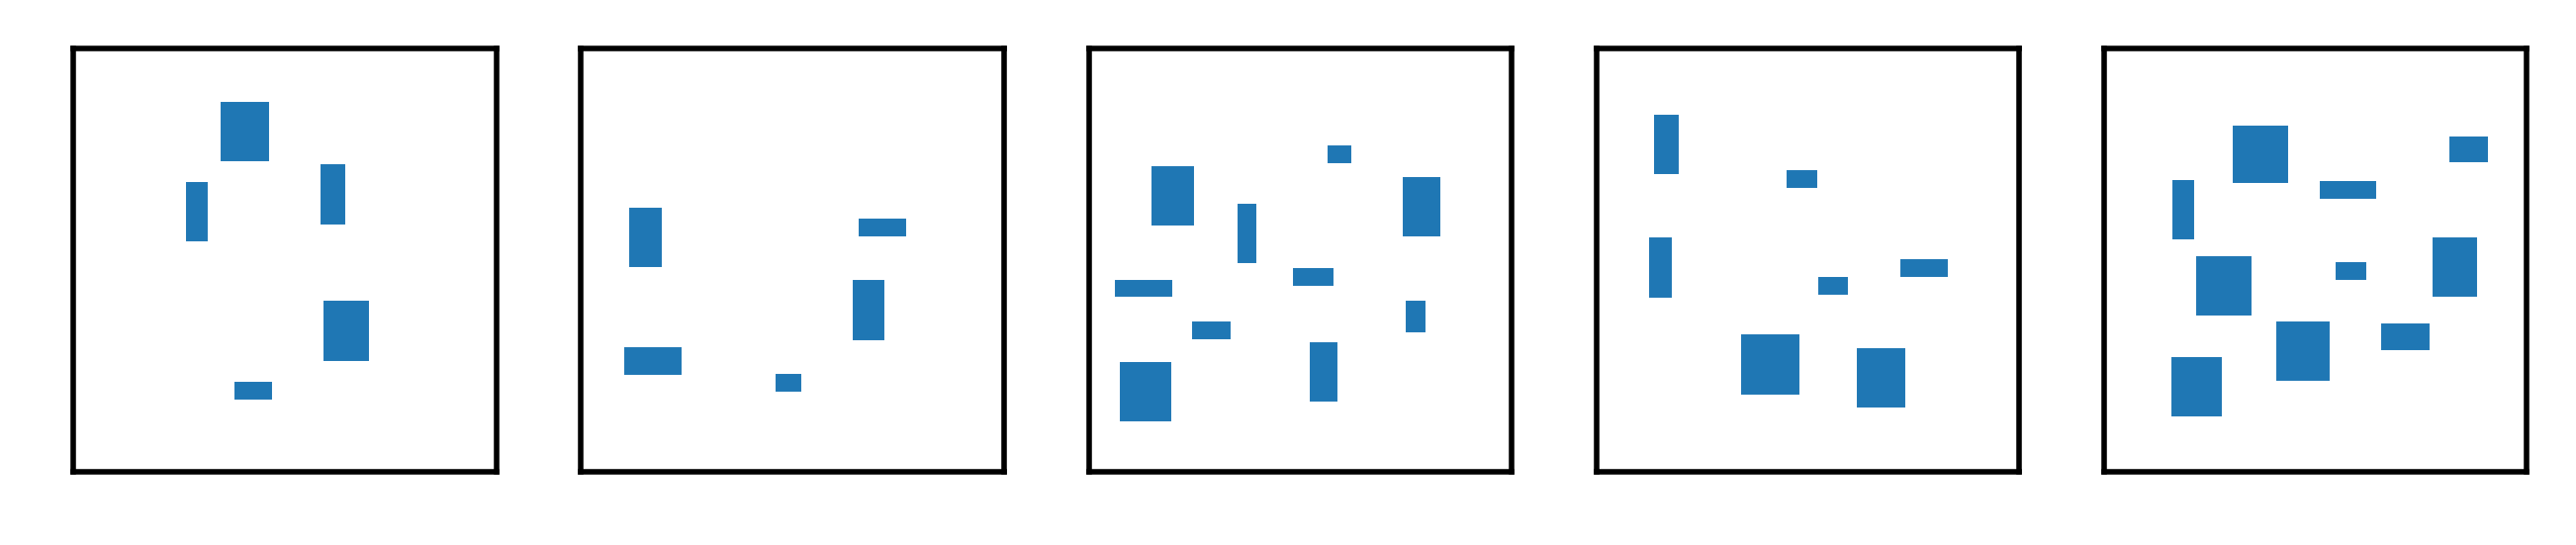
\includegraphics[width=.8\linewidth]{figures/content/chapter4/obstacles.png}
  \caption{随机生成的仿真训练环境}
  \label{fig:4_3}
\end{figure}
在训练过程中，智能体被建模为一个全连接网络，有 3 个隐藏层，每层 512 个单元。
除输出层外，每个全连接层后都接有 ReLU\citen{fred2018deep}激活函数。
我们使用Adam\citen{reyad2023modified}优化器，学习率为 lr。
每D个训练阶段进行一次更新，从大小为E的经验回放缓冲区中抽取批量大小为B的样本。
使用的超参数与值列于表\ref{tab:hyperparams}。

\begin{table}[htbp]
  \centering
  \begin{tabular}{ll|ll|ll|ll}
    \hline
    $lr$ & $2 \times 10^{-4}$ & $v_m$ & $1\ [m/s]$ & $D$ & $5$ & $N, N'$ & $16$ \\
    $E$ & $5 \times 10^{4}$ & $r_d$ & $0.05\ [m]$ & $K$ & $64$ & $m$ & $3$ \\
    $\gamma$ & $0.99$ & $d_f$ & $0.1\ [m]$ & $B$ & $32$ & $b$ & $9$ \\
    $T$ & $0.1\ [s]$ & $d_s$ & $0.2\ [m]$ & $H$ & $200$ & $\eta$ & $0.5$ \\
    \hline
  \end{tabular}
  \caption{超参数的符号与值}
  \label{tab:hyperparams}
\end{table}

在无人机导航仿真评估中，为了展示我们算法的有效性，我们将ART-IQN与具有多个风险倾向$\alpha=\{0.1,0.25,0.5,0.75,1.0\}$的IQN进行比较。
此外，我们还训练了一个DQN智能体作为对照，训练过程与所提出的算法相同。
我们比较了不同智能体在不同环境下的平均回合返回值、成功率、碰撞率和平均导航时间。
具体来说，评估在三组环境上进行，每组环境包含100个不同的随机环境，每个智能体的节点数分别为$n_{obs}=\{2,6,12\}$。

\begin{table}[htbp]
  \centering
  \caption{CVaR 性能指标对比}
  \label{tab:cvar_comparison}
  \begin{tabular}{|c|c|*{9}{c|}}
    \hline
    \multirow{2}{*}{方法} & \multirow{2}{*}{CVaR} & \multicolumn{3}{c|}{成功率} & \multicolumn{3}{c|}{碰撞率} & \multicolumn{3}{c|}{导航时间 [s]} \\
    \cline{3-11}
    & & n=26 & n=12 & n=6 & n=26 & n=12 & n=6 & n=26 & n=12 & n=6 \\
    \hline
    DQN  & - & 0.85 & 0.65 & 0.56 & 0.13 & 0.31 & 0.39 & 5.23 & 8.11 & 8.34 \\
    \hline
    \multirow{5}{*}{IQN} & 0.1 & 0.87 & 0.74 & 0.59 & 0.09 & 0.15 & 0.17 & 5.41 & 12.52 & 18.52 \\
    & 0.25 & 0.88 & 0.72 & 0.67 & 0.10 & 0.17 & 0.25 & 5.31 & 10.23 & 13.23 \\
    & 0.5 & 0.87 & 0.73 & 0.66 & 0.11 & 0.19 & 0.28 & 5.30 & 8.46 & 9.46 \\
    & 0.75 & 0.84 & 0.69 & 0.62 & 0.13 & 0.22 & 0.31 & 5.25 & 8.57 & 8.60 \\
    & 1.0 & 0.86 & 0.67 & 0.57 & 0.12 & 0.30 & 0.41 & 5.12 & 7.89 & 8.05 \\
    \hline
    ART-IQN & - & 0.87 & 0.77 & 0.70 & 0.11 & 0.17 & 0.15 & 5.32 & 8.26 & 11.76 \\
    \hline
  \end{tabular}
\end{table}

表\ref{tab:cvar_comparison}通过对比DQN、不同风险偏好下的 IQN 以及ART-IQN，展示了定量实验结果。
在所有测试环境中，DQN的表现与风险中性的IQN相近。
当障碍物数量$n_{obs}=2$时，环境相对简单，所有智能体均能以较高的成功率和较低的碰撞率完成导航任务。
当$n_{obs}=6$时，采用较低CVaR值的IQN智能体相比高CVaR值的智能体碰撞率更低，但其任务完成时间更长，超时率也更高。
相比之下，ART-IQN 在成功率达到0.77的同时，保持了较低的碰撞率，且平均导航时间仅比风险中性策略长出0.37秒。
在$n_{obs}=12$的情况下，所有智能体的平均回报和成功率均有所下降。
这一下降可归因于智能体所面临的严重部分可观测性问题。在低CVaR设置下超时情况更常见，而在高CVaR设置下碰撞更为频繁。
相比之下，ART-IQN 在成功率和碰撞率方面均表现最佳，同时导航时间也维持在合理范围内。

\begin{figure}[htbp]
  \centering
  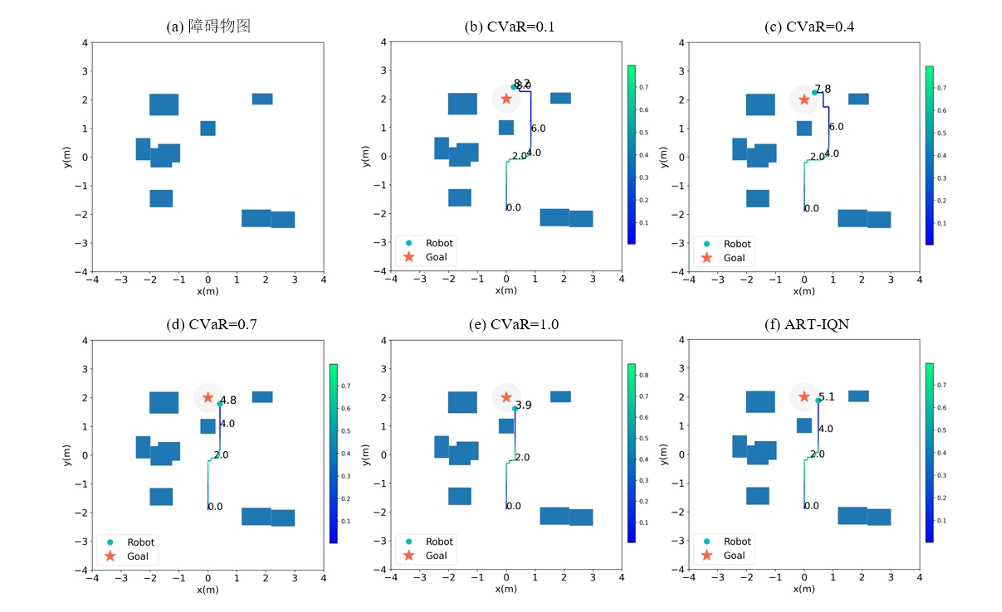
\includegraphics[width=.9\linewidth]{figures/content/chapter4/uvasimulation.png}
  \caption{不同风险倾向的无人机行为和导航时间比较}
  \label{fig:4_4}
\end{figure}

我们选取一次随机生成障碍物数量为9个的实验结果作为典型样例进行定行分析，如图\ref{fig:4_4}所示。
其中图\ref{fig:4_4}（a）是障碍物图，图\ref{fig:4_4}（b）-图\ref{fig:4_4}（e）是具有不同CVaR的IQN模型结果，图\ref{fig:4_4}（f）是ART-IQN模型结果，路线上的颜色表示飞行时的速度，数字表示飞行路线的长度。
当CVaR的数值为1时，无人机会以优先到达目的地为目标，而忽略了因接近障碍物导致的碰撞风险，所以在图\ref{fig:4_4}（e）中，无人机后半程以紧贴方形障碍物线路飞行，并以最短的3.9米总路程到达终点。
随着CVaR数值的下降，无人机会逐渐提高与障碍物碰撞的警觉性，这会在周围有障碍物的情况下，优先保障无人机与障碍物处于一定的安全距离，但牺牲了飞行的速度以及可能导致更远的飞行路线，甚至在CVaR数值为0.4和0.1的情况下，无人机在接近终点时收到终点左侧矩形障碍物影响，都出现不同程度进一步再向y轴正方向飞行的情况。

相比之下，在图\ref{fig:4_4}（f）中，ART-IQN模型的无人机通过动态调整CVaR，在避障效率与风险控制间取得平衡，其路径在周围障碍物变多时保持较低的速度以及一定的距离，当周围障碍物变少时，提高飞行的速度。
在飞行刚开始时，飞机速度偏小，这是因为刚开始还并不了解周围的环境，不确定性较高，随着飞机向前接近目标点方向飞行，周围障碍物稀松并且距离较远，速度开始加快，当发现坐标点大约为（0，1）的障碍物时，飞机进行避障处理且降低飞行速度，直至抵达飞行终点。


\begin{figure}[htbp]
  \centering
  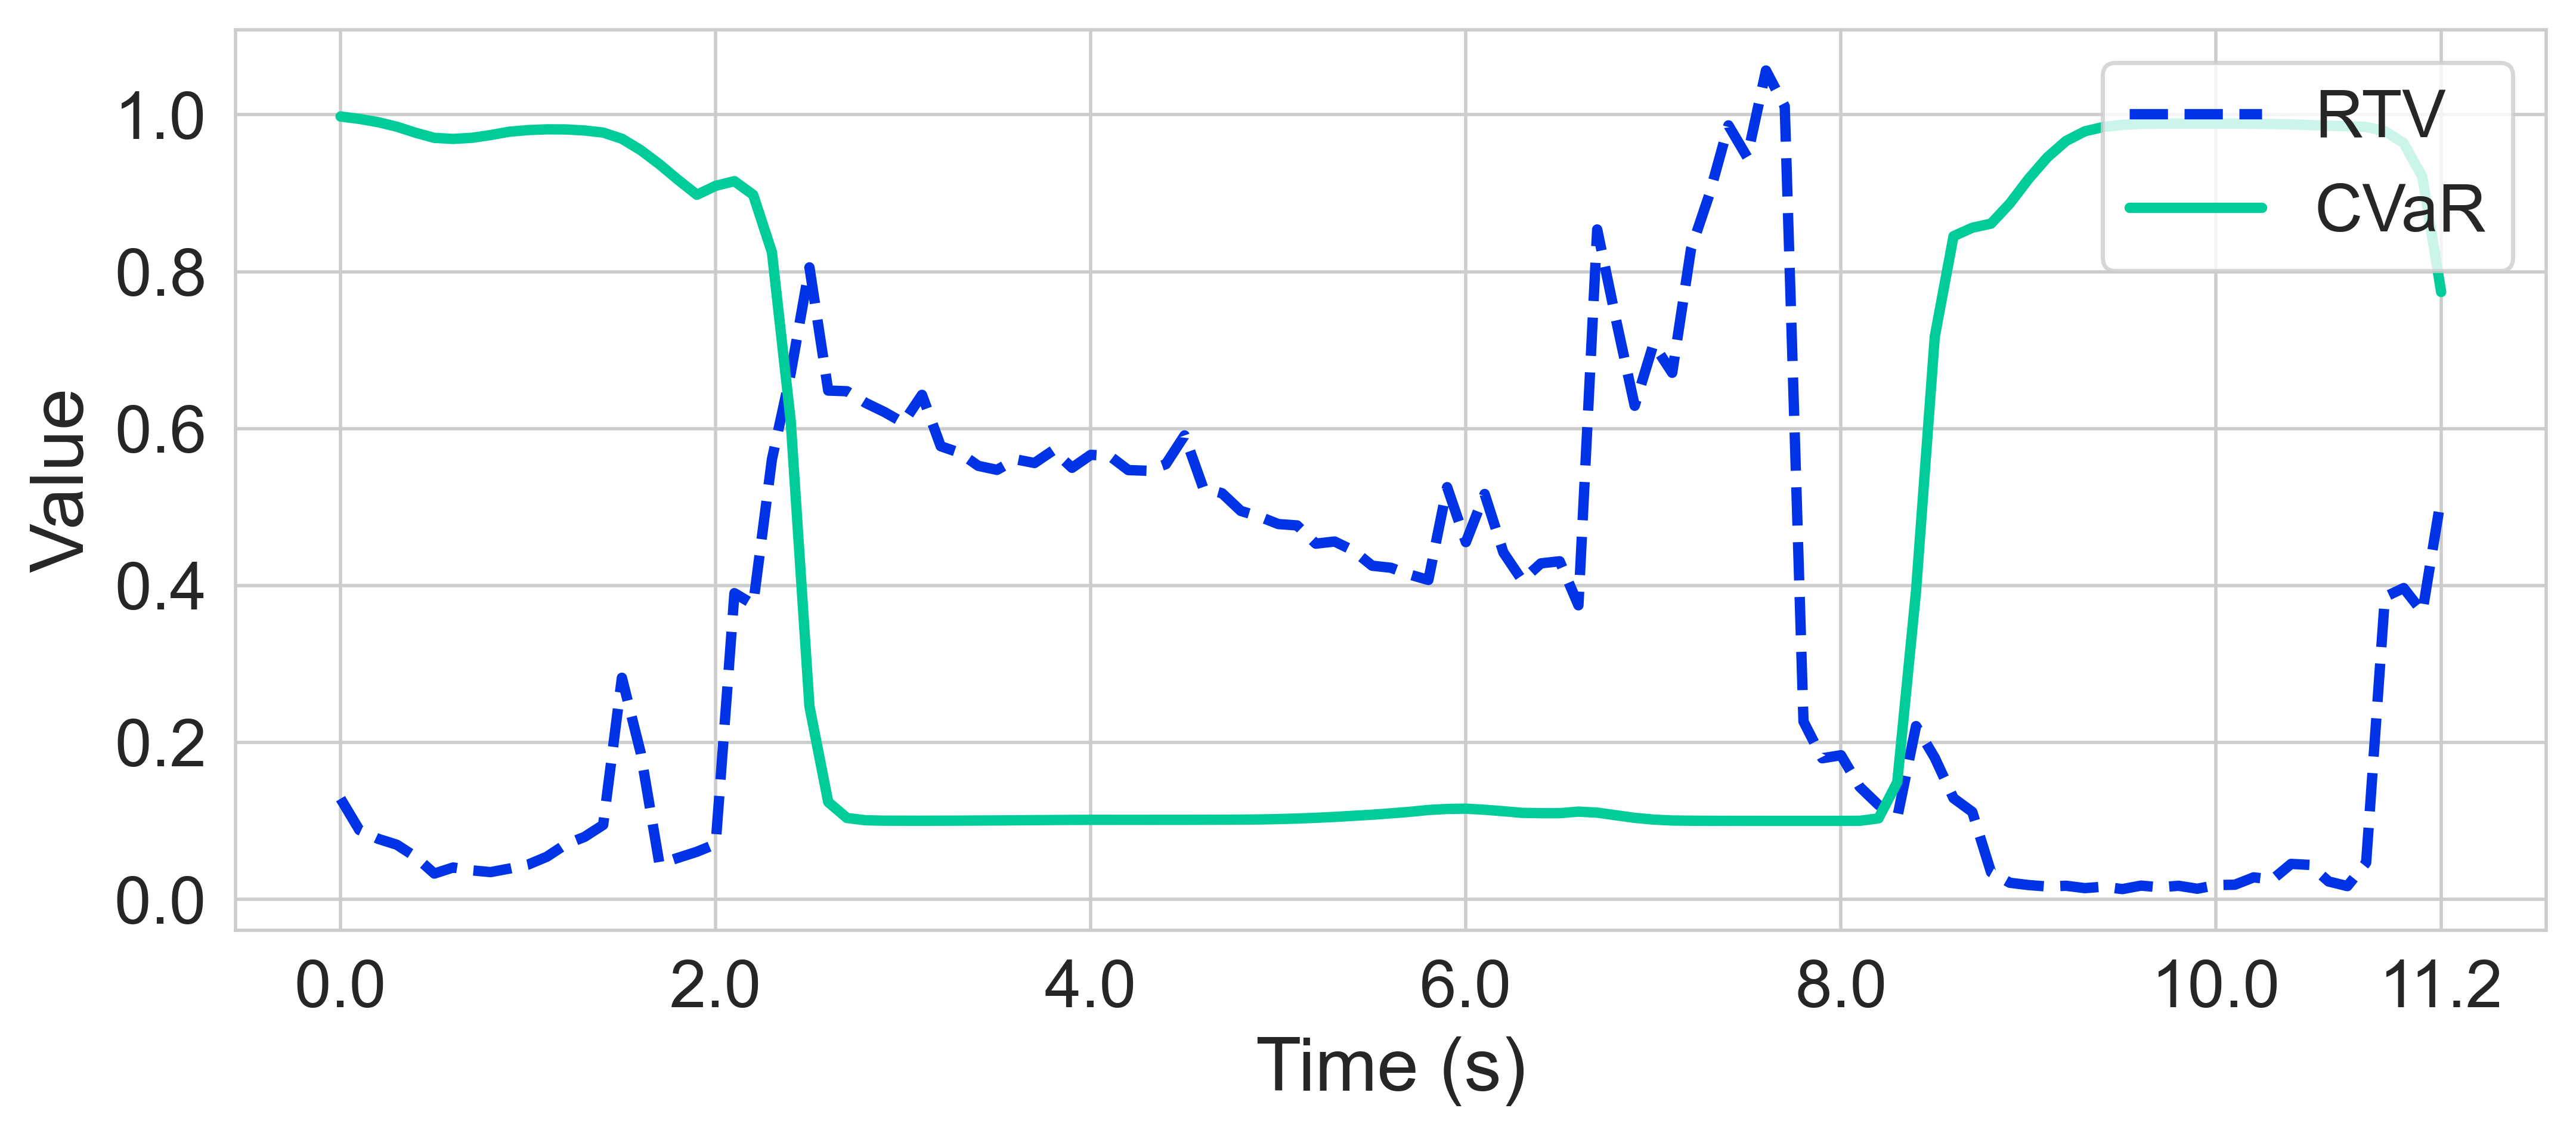
\includegraphics[width=.8\linewidth]{figures/content/chapter4/tcv.png}
  \caption{右截断方差（RTV）和自适应条件风险价值（CVaR）的关系。}
  \label{fig:4_5}
\end{figure}
图\ref{fig:4_5}展示了图\ref{fig:4_4}(f)轨迹中右截断方差和自适应条件风险价值的变化情况。
无人机初始时采用风险中性的自适应条件风险价值参数1.0，这是因为在尚未熟悉环境时，它采取风险中性的策略。
在0至2秒期间，由于当前环境不确定性较低，无人机以最大速度进行风险中性飞行。
大约在2至8秒期间，由右截断方差估计的内在不确定性增加并维持在高位，导致CVaR值下降，这对应于图\ref{fig:4_4}(f)中间区域表现出的风险规避行为。
当右截断方差从8秒开始下降并维持在较低水平直至回合结束，自适应条件风险价值值随之升高，使无人机重新采用风险中性策略，以高效方式抵达目标点。
这清晰地表明，在导航过程中，无人机能够根据环境不确定性动态调整其风险倾向：当不确定性增加时表现出风险规避行为，当环境不确定性降低时则转向风险中性策略。
\section{基于分布式强化学习的导航模型部署与验证}
在前文中，我们已经基于分布式强化学习方法完成了无人机自主导航模型的训练与验证，并在仿真环境中取得了较好的性能表现。
然而，仿真环境与实际嵌入式平台在计算资源、功耗约束以及实时性要求等方面存在显著差异，因此有必要将训练得到的模型进一步压缩与优化，并部署至实际飞行平台上进行验证。

本节面向资源受限的嵌入式系统，针对所训练的分布式强化学习导航模型开展轻量化处理与工程化部署。
首先，借助 X-CUBE-AI 工具链对训练好的神经网络模型进行自动化优化与部署转换。
该工具通过权重量化、算子融合以及内存调度优化等方法，在尽可能保持模型决策性能的前提下，有效降低模型的存储开销与计算复杂度，从而提升模型在嵌入式平台上的推理效率。
在模型部署方面，本文将优化后的神经网络模型烧录并运行于Adhoc Deck扩展板所搭载的STM32H743微控制器上，实现端侧推理计算。Crazyflie 2.1主控负责底层飞控与姿态稳定控制，而Adhoc Deck作为协处理单元，负责执行强化学习策略推理，并根据当前环境状态输出导航决策指令。两者通过通信接口进行数据交互，从而构建“飞控执行—边缘决策”协同架构，实现计算与控制的功能解耦。

最后，在Crazyflie 2.1微型无人机平台上开展真实环境飞行实验，对所部署模型的导航性能、环境适应能力以及实际运行效率进行综合评估。实验结果表明，经过轻量化处理后的模型能够在资源受限的嵌入式硬件上稳定运行，并满足实时导航任务的需求。

本节内容结构如下：首先介绍部署平台与相关工具；其次详细阐述网络模型的量化方法与具体部署流程；最后给出真机实验结果，并对模型在实际环境中的表现进行分析与讨论。
\subsection{部署工具与部署平台}
在本小节中我们使用的部署工具为X-CUBE-AI，它是由 STMicroelectronics提供的一个重要扩展工具包，隶属于 STM32Cube.AI生态体系，主要面向嵌入式边缘智能应用的开发与部署。该工具基于 STM32CubeMX 开发环境，能够实现从模型转换、性能优化到嵌入式部署的全流程支持，显著降低了深度学习模型在资源受限设备上的落地难度。

具体而言，X-CUBE-AI 支持将主流深度学习框架（如 TensorFlow、Keras 等）中训练好的神经网络模型自动转换为高效的ANSI C 代码，从而使其能够在STM32系列微控制器上运行。
转换过程中，工具会结合目标硬件平台的存储资源、算力约束以及功耗需求，对模型结构进行裁剪与优化，包括权重量化、内存复用以及运算融合等，以提高推理效率并降低资源占用。
在面向集成Neural-ART加速器的硬件平台时，X-CUBE-AI 进一步提供了针对专用神经网络处理单元的优化支持。
具体来说，该工具会对神经网络中的各类算子进行细粒度分析，在算子级别生成对应的微代码，并尽可能将计算任务映射至Neural-ART加速器执行，从而充分发挥硬件加速能力。
当某些算子无法被 NPU支持时，系统会自动将其调度回通用CPU执行，实现异构计算资源之间的协同调度。
这种基于算子级别的动态调度机制，在保证模型功能完整性的同时，最大程度提升了整体推理性能和执行效率。
此外，X-CUBE-AI还支持将生成的优化推理库无缝集成到用户工程中，并提供完整的接口函数用于模型初始化、输入输出管理及推理调用。这使得开发者能够在不深入底层实现细节的情况下，将人工智能算法快速部署到嵌入式系统中，实现从云端训练到端侧推理的高效迁移。
\begin{figure}[htbp]
  \centering
  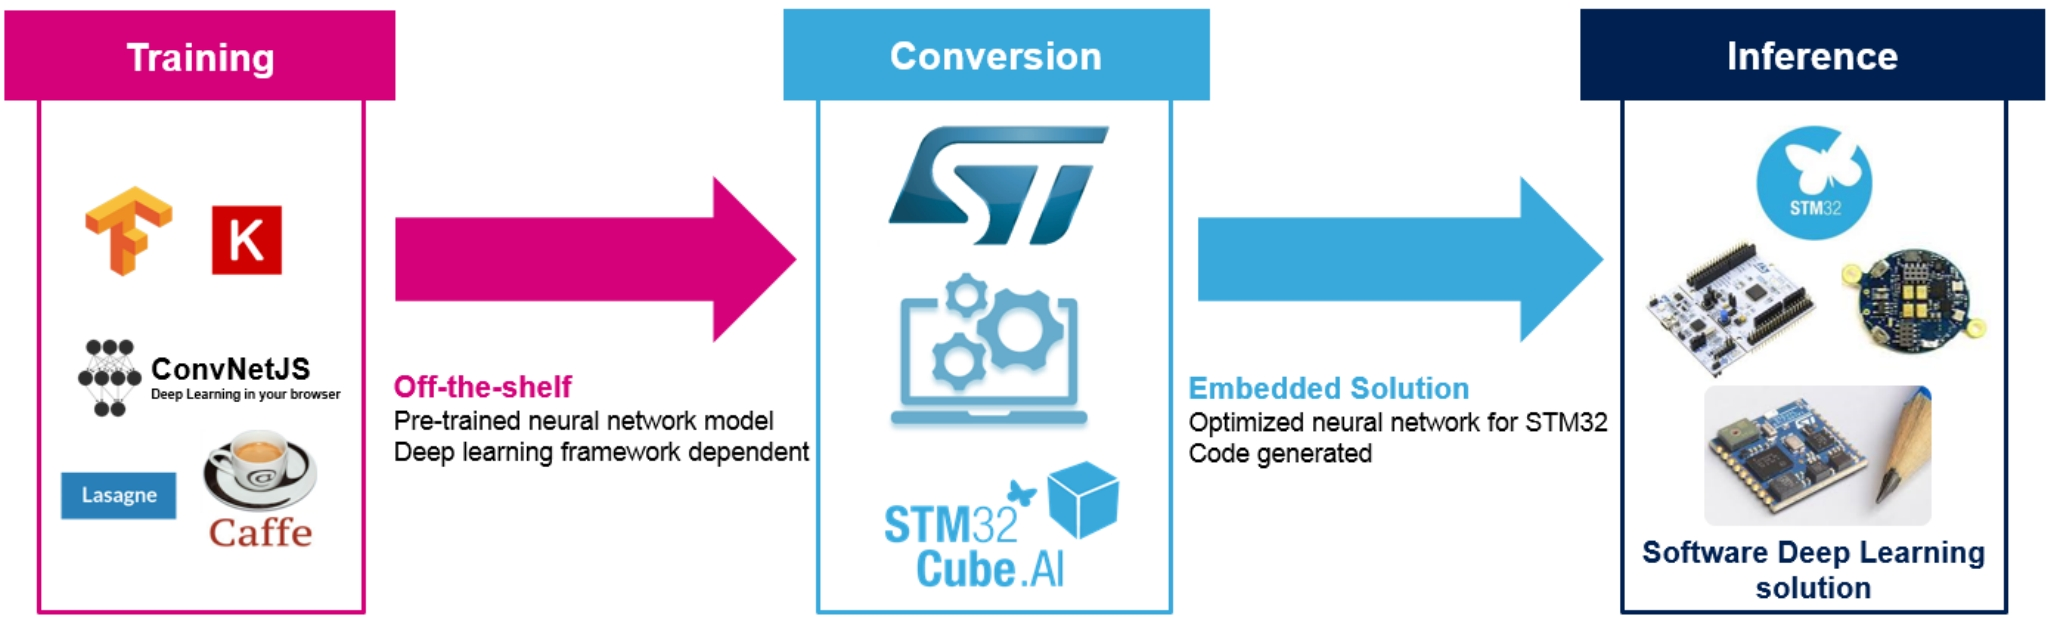
\includegraphics[width=.8\linewidth]{figures/content/chapter4/CUBEAI.jpeg}
  \caption{ X-CUBE-AI 概述}
  \label{fig:4_6}
\end{figure}


本文实验最终将优化后的神经网络模型部署于 Adhoc Deck 扩展板硬件平台上。
该扩展版以 STM32H743VIH6 微控制器为核心，辅以外部Flash存储器与FRAM非易失性存储器，形成了一套兼顾计算性能、存储容量与数据可靠性的嵌入式系统。
STM32H743VIH6 基于ARM Cortex-M7内核，主频最高可达480 MHz，具备较强的浮点运算能力和丰富的片上外设资源，可满足复杂算法在嵌入式环境下的实时运行需求。

在存储设计方面，系统采用多层次存储架构。
首先，微控制器内部集成2MB片上Flash存储空间。该存储器采用双存储块结构，每个存储块容量为1MB，并进一步划分为多个扇区。这部分存储空间用于存储系统核心程序与基础配置，并通过逻辑划分实现不同功能区域的隔离，包括Bootloader区、主固件区、配置区以及用户数据区。其中，Bootloader负责系统启动及固件更新管理，主固件区用于存储应用程序，配置区用于保存系统参数，而用户数据区则支持运行过程中的数据存储。

在存储体系设计方面，系统采用分层化的多级存储架构。首先，微控制器内部集成 2MB 片上 Flash 存储空间。该存储器采用双存储体（Dual-Bank）结构，每个存储体容量为 1MB，并进一步划分为多个扇区（Sector）。基于该片上 Flash，系统实现了功能分区，包括 Bootloader 区、主固件区、配置区以及用户数据区。其中，Bootloader 区用于系统启动与固件升级管理，主固件区用于存储应用程序，配置区用于保存系统参数，而用户数据区则用于支持运行过程中的数据存储需求。此外，系统预留独立的 Flash 扇区作为临时存储区，在固件升级过程中用于缓存新版本固件，从而实现安全可靠的在线升级机制。

为进一步提升系统的数据存储能力，Adhoc Deck 扩展板引入了外部 Flash（W25Q64），用于存储大容量数据，如运行日志、轨迹信息以及扩展资源文件。同时，系统集成了 FRAM（FM25CL64）作为高可靠性存储单元。相比传统 Flash 存储器，FRAM 具有更高的写入速度和极高的擦写寿命，且无需擦除即可直接写入，因而特别适用于频繁更新的关键数据（如系统状态与控制参数）的存储场景。

综上，Adhoc Deck 扩展板通过片上 Flash、外部 Flash 与 FRAM 的协同设计，在存储容量、访问效率及数据可靠性之间实现了有效平衡。其中，片上 Flash 保障系统运行与升级过程的安全性，外部 Flash 提供大容量数据支持，而 FRAM 则满足高频写入与关键数据保护需求。该多层次存储架构为后续算法的稳定运行与数据处理提供了坚实的硬件基础。

\begin{figure}[htbp]
    \centering
    \subfloat[正面]{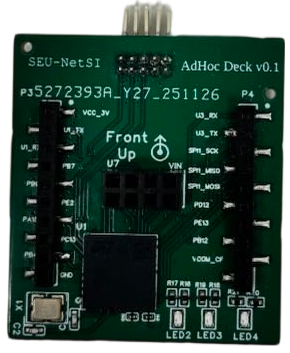
\includegraphics[width=.4\textwidth]{figures/content/chapter4/Adhoc正面.png}}
    \quad
    \subfloat[反面]{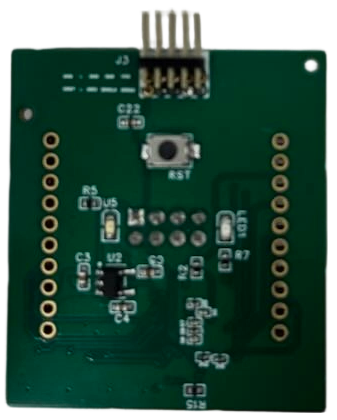
\includegraphics[width=.4\textwidth]{figures/content/chapter4/Adhoc反面.png}}
    \caption{部署平台：Adhoc Deck}
    \label{fig:4_7}
    \end{figure}

\subsection{网络模型的量化与部署}

在完成分布式强化学习模型的训练后，为实现其在嵌入式平台上的高效部署，需要将原始基于PyTorch框架的模型转换为硬件可执行的中间表示格式。为此，本文采用 ONNX（Open Neural Network Exchange）作为模型转换的中间桥梁，以实现模型从训练环境向嵌入式推理引擎的平滑迁移。

具体而言，首先对原始的 IQN模型进行结构封装，构建适用于导出的推理模型。在不改变原始网络结构与参数的前提下，对模型的前向传播过程进行显式展开，使其计算图能够被ONNX正确解析与表达。在该封装过程中，重点保留并规范化如下关键计算流程：状态特征提取、分位数特征映射、状态与分位数特征融合，以及分布式Q值估计。其中，分位数嵌入模块采用余弦基函数对采样分位点进行映射，并通过全连接层投影至高维特征空间，从而有效刻画动作价值的分布特性，增强模型对不确定性的表达能力。

为验证模型转换过程的正确性与稳定性，本文在Python环境下对转换前后的模型输出进行一致性检验。具体方法为：构造相同输入，分别输入至 PyTorch 模型与 ONNX 模型中，并计算两者输出 Q 值之间的最大绝对误差。实验结果表明，转换前后模型输出的最大误差控制在 $10^{-5}$ 以内，表明模型在转换过程中未引入显著数值偏差，具备良好的数值一致性，为后续嵌入式平台部署提供了可靠保障。图\ref{fig:4_8}展示了压缩后模型的网络图。
 \begin{figure}[htbp]
  \centering
  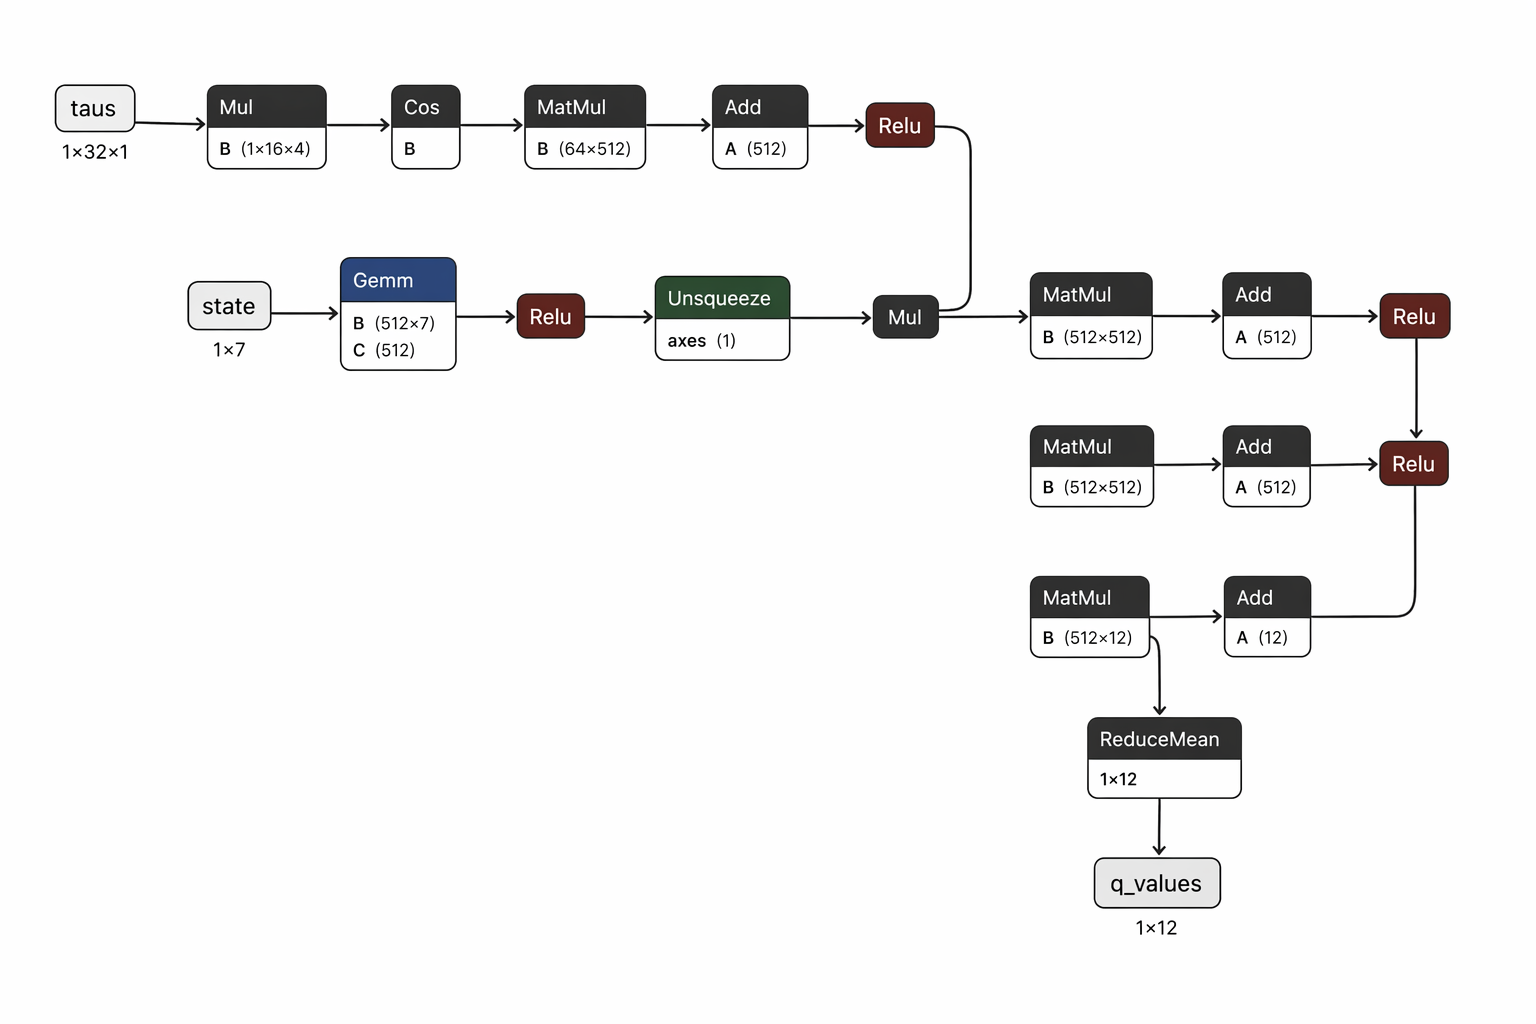
\includegraphics[width=.7\linewidth]{figures/content/chapter4/iqn_native.png}
  \caption{转换后的网络模型图}
  \label{fig:4_8}
\end{figure}

本文基于 STM32Cube.AI 提供的模型转换与部署工具链，对训练完成的模型进行了多层次优化处理。
整体而言，该优化过程并非单一压缩策略，而是由计算图优化、算子融合、权重量化、权重压缩、内存复用以及推理内核优化等多种技术协同构成。
首先，在模型转换阶段，通过对计算图进行静态分析，执行常量折叠与冗余节点消除等操作，将训练阶段中可预计算的部分提前固化，从而减少运行时计算负担；
同时，通过算子融合技术，将卷积层与批归一化层、激活函数等进行等效合并，在不改变模型表达能力的前提下减少中间张量的生成与存储开销，提高执行效率。
在此基础上，引入量化机制，将原始的 32 位浮点参数映射为低比特定点表示，显著降低模型参数存储规模，并使推理过程能够利用嵌入式处理器中的定点运算单元，从而在保证精度可控的前提下提升计算效率。

在上述优化手段中，权重压缩是降低模型 ROM 占用的关键技术之一，其具体实现过程如图\ref{fig:4_9}所示。原始网络模型中，各层权重与偏置参数（如 W1.conv、W2.dense、W3.dense）通常以 float32 形式分散存储，其总体大小由参数数量与数据精度共同决定，对应图中的未压缩存储结构（Un-compressed ROM size）。针对这一问题，CUBE-AI 首先对各层参数进行结构化重排，将不同层的权重与偏置按照统一顺序拼接为连续的内存块（memory chunk），从而提升数据访问的局部性，并为后续压缩提供统一的数据组织形式。在此基础上，结合量化后的低比特表示，对权重数据进行进一步压缩编码，将原始高精度参数映射为紧凑的定点表示，并通过统一格式进行集中存储。由图中“W′ compressed layer”可以看出，压缩后的权重不再与原始层一一对应，而是以压缩块形式重新组织，其中标注的“×4”表示相应权重存储规模约缩减至原始的四分之一，而“×1”则表示该部分压缩收益较低，基本保持原始比例。该过程本质上通过减少冗余表示与优化存储结构，实现参数的高效编码。

\begin{figure}[htbp]
  \centering
  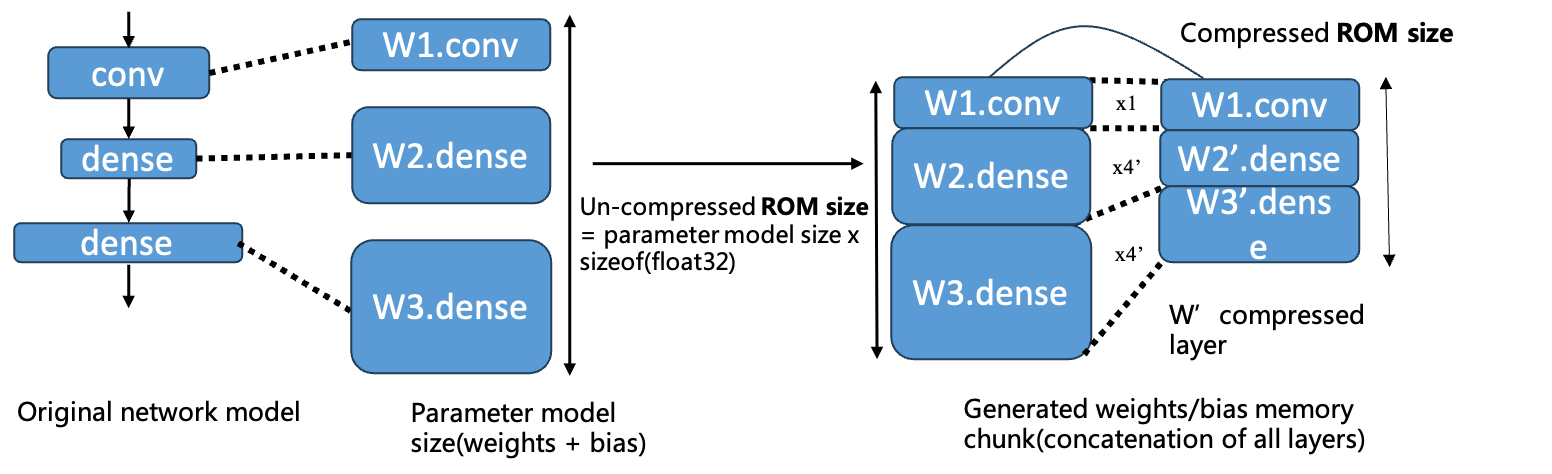
\includegraphics[width=.8\linewidth]{figures/content/chapter4/compressTheory.png}
  \caption{CUBE-AI权重压缩}
  \label{fig:4_9}
\end{figure}

在推理执行阶段，压缩后的权重通常以连续数组形式存储于 Flash 中，并在计算过程中按需读取，直接以定点形式参与运算或通过轻量级解码恢复必要精度，从而避免频繁的浮点转换操作，在保证计算正确性的同时兼顾存储效率与执行效率。通过上述机制，模型参数存储规模通常可降低至原始 float32 表示的约 1/4 甚至更低，显著缓解嵌入式平台的存储压力。此外，为进一步降低运行时内存占用，CUBE-AI 通过生命周期分析对中间张量进行内存复用，将不同计算阶段的缓冲区映射至同一物理地址，从而减少 RAM 使用量；同时采用静态内存分配策略，在编译阶段确定所有张量的内存布局，避免动态分配带来的额外开销与内存碎片问题。在推理执行层面，通过调用针对 ARM Cortex-M 架构优化的高效计算内核（如基于 SIMD 与 DSP 指令的实现），进一步提升模型运行速度。综上所述，该模型压缩与优化过程从存储表示、计算结构及执行机制多个层面协同作用，在保证模型精度基本稳定的前提下，大幅降低了模型对嵌入式硬件资源的需求，为复杂深度学习模型在资源受限环境中的高效部署提供了有效支撑。

如图\ref{fig:4_10}所示，给出了经仿真验证后的训练模型在压缩优化后的复杂度分析结果。
基于 STM32Cube.AI 生成的报告可知，模型单次推理的乘加运算次数（MACC）为18\allowbreak,033\allowbreak,384次，其中计算开销主要集中在中间的矩阵乘法层，单层占比约为 46.5\%，而激活函数及加法等操作的计算占比较低。
存储方面，模型在 Flash（ROM）中的占用为 572,636 Byte（约 559.21 KiB），全部由权重参数构成，表明量化与权重压缩已有效降低存储规模。运行内存方面，推理过程占用 RAM 为 34,816 Byte（约 34.00 KiB），主要用于中间激活值存储，输入输出占用极小且已包含其中。总体来看，压缩后的模型在计算复杂度、存储占用及内存使用之间实现了良好平衡，能够满足嵌入式平台的部署需求。

\begin{figure}[htbp]
  \centering
  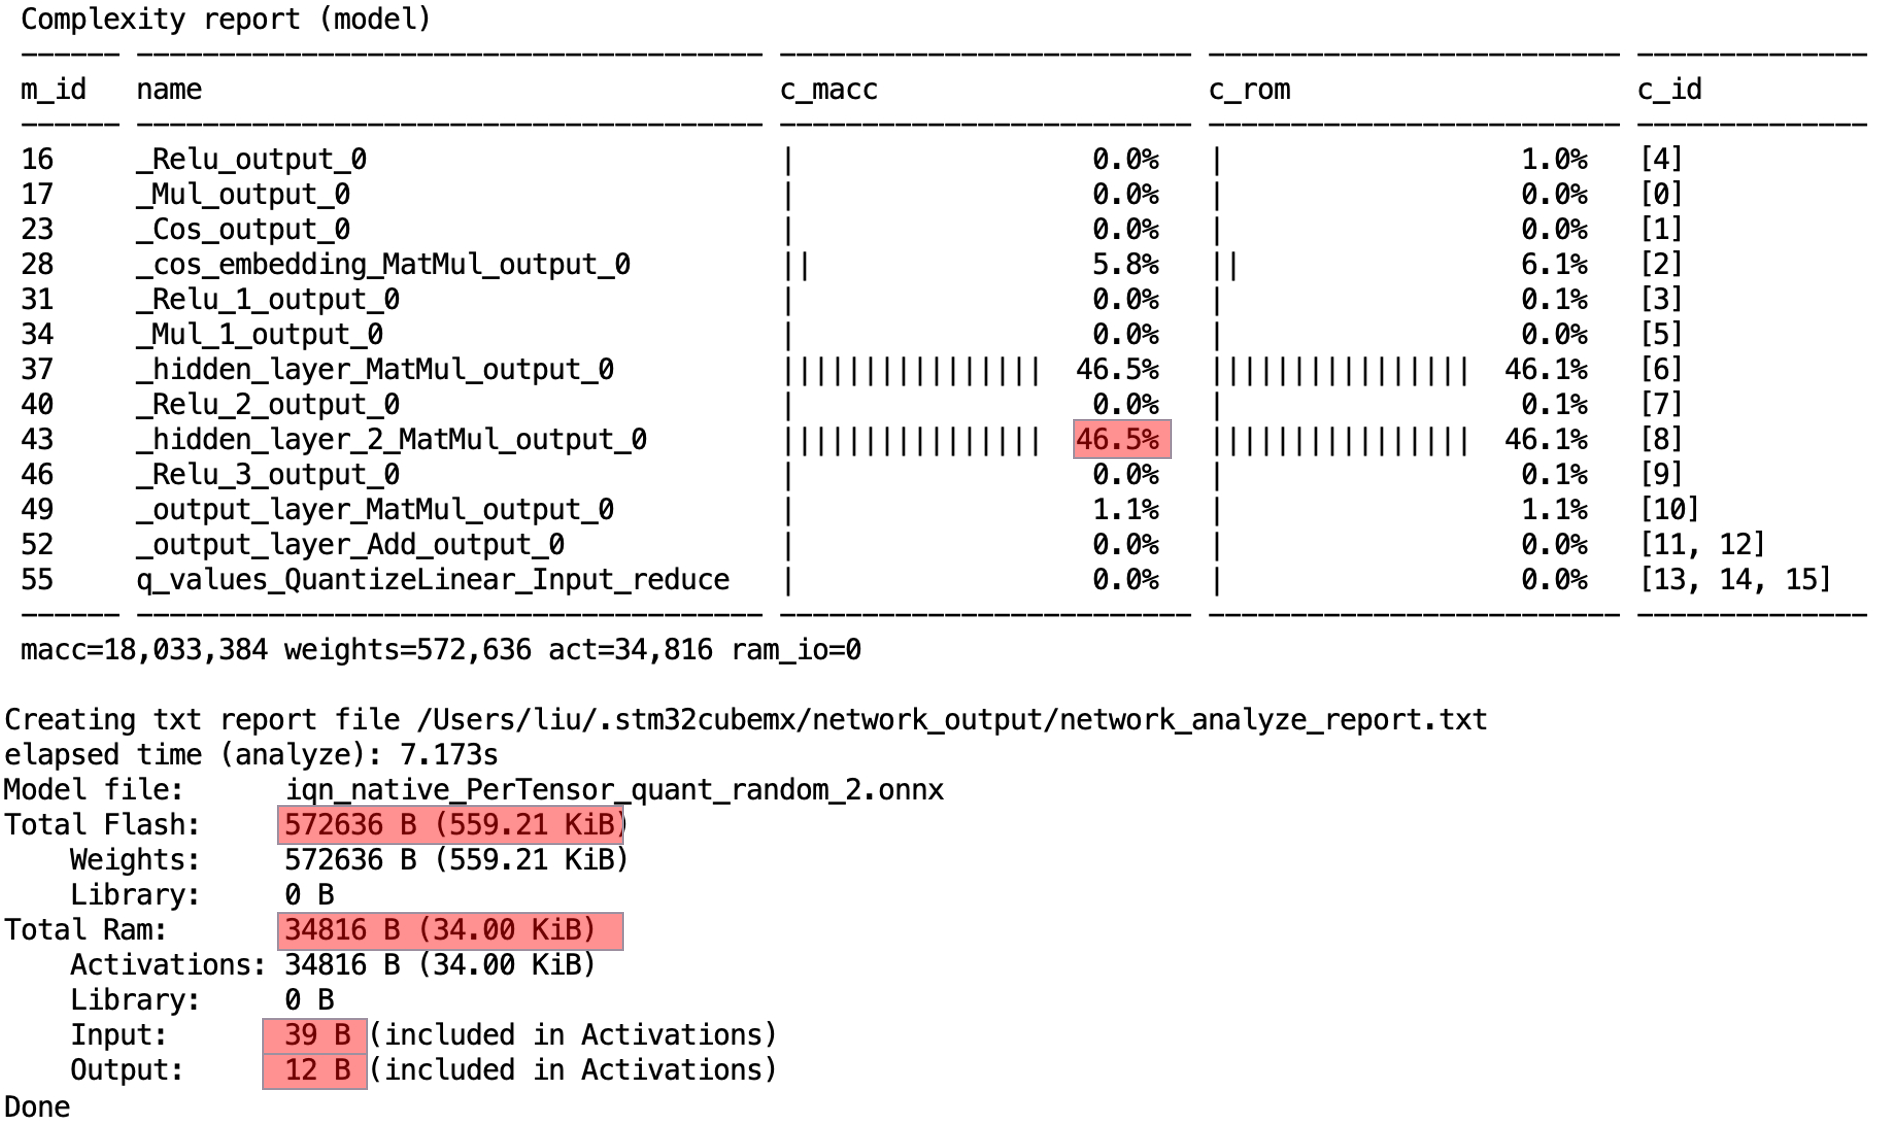
\includegraphics[width=.8\linewidth]{figures/content/chapter4/AIcompression.png}
  \caption{模型压缩结果}
  \label{fig:4_10}
\end{figure}
针对压缩后的模型，其具体的嵌入式部署方法如图\ref{fig:4_11}所示。
系统以 Adhoc Deck 扩展板为核心计算单元，用于分别存储运行时数据与压缩后的神经网络模型参数。
在该硬件平台上部署经优化后的IQN模型，实现飞行过程中的实时决策推理。

在模型部署流程中，首先将训练并压缩后的模型烧录至 Flash 存储器中，系统运行时由主控处理器加载相关参数并执行推理计算。模型以无人机当前状态信息作为输入，输出对应的动作价值估计或控制指令，从而实现对飞行行为的实时决策控制。整个推理过程在嵌入式端本地完成，无需依赖外部计算资源，从而保证系统的实时性与自主性。
在感知与通信方面，系统通过 Multi-ranger Deck 获取周围障碍物的距离信息，该模块通过I2C接口与无人机进行数据交互，实现环境感知输入的实时更新。
同时，外部定位系统采用 Vicon 动作捕捉系统，通过计算机端处理后生成高精度位姿数据，并经由 2.4G Crazyradio PA 无线通信模块发送至无人机，实现定位信息的闭环反馈。
嵌入式系统通过 UART 接口实现Adhoc Deck与无人机进行数据交互，实现模型输入输出与飞控控制指令之间的传递。
从整体数据流来看，系统形成了“环境感知—状态获取—模型推理—控制输出”的闭环结构：一方面，多源传感器（如测距模块与定位系统）提供实时环境与位置信息；另一方面，嵌入式端部署的 IQN 模型对输入状态进行推理，输出控制策略，并通过通信接口反馈至无人机执行机构，从而实现自主决策与避障控制。

综上所述，该部署方案充分结合了嵌入式计算平台与外部感知系统的优势，通过在资源受限的硬件环境中实现强化学习模型的高效推理，构建了一个具备实时性与自主性的无人机智能控制系统，为后续复杂环境下的自主导航与决策提供了可靠基础。
\begin{figure}[htbp]
  \centering
  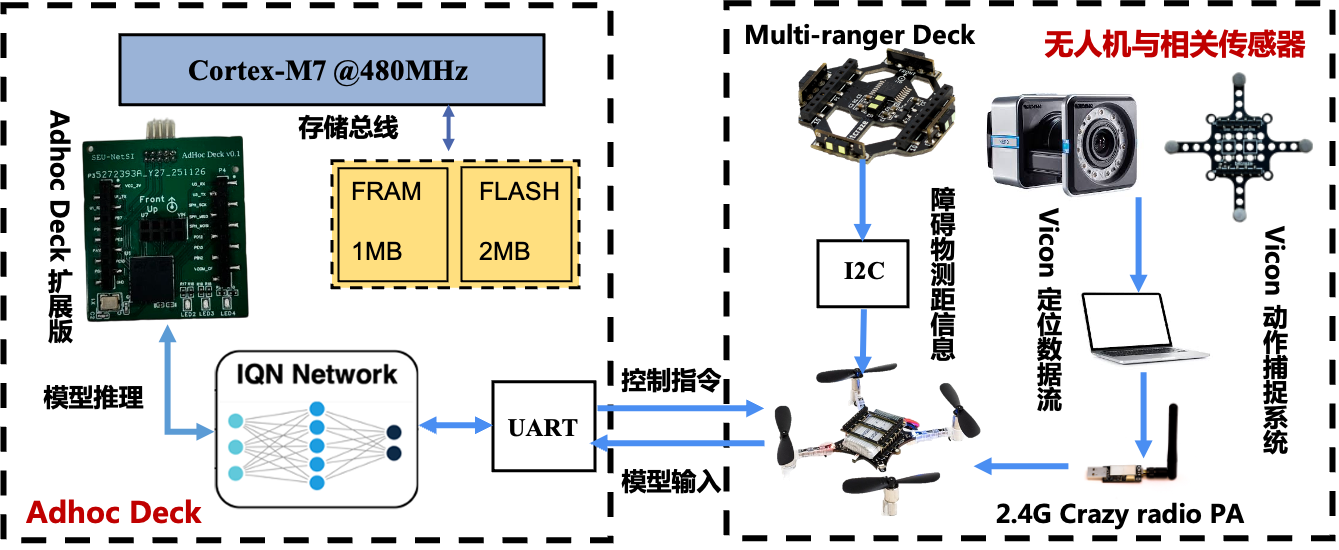
\includegraphics[width=.8\linewidth]{figures/content/chapter4/Adhoc与无人机交互.png}
  \caption{Adhoc Deck与无人机及其相关传感器交互}
  \label{fig:4_11}
\end{figure}

\subsection{真机实验结果分析}
本节基于上述算法与系统设计开展真机实验，以验证所提出强化学习导航算法在实际系统中的可行性与实时性。
首先对无人机硬件平台及其相关配置进行介绍，如图\ref{fig:4_12}所示，实验平台基于开源微型四旋翼无人机Crazyflie 2.1，并结合扩展计算模块Adhoc Deck构建边缘推理系统，实现模型在嵌入式端的在线决策能力与无人机导航功能。具体配置如下

\begin{figure}[htbp]
  \centering
  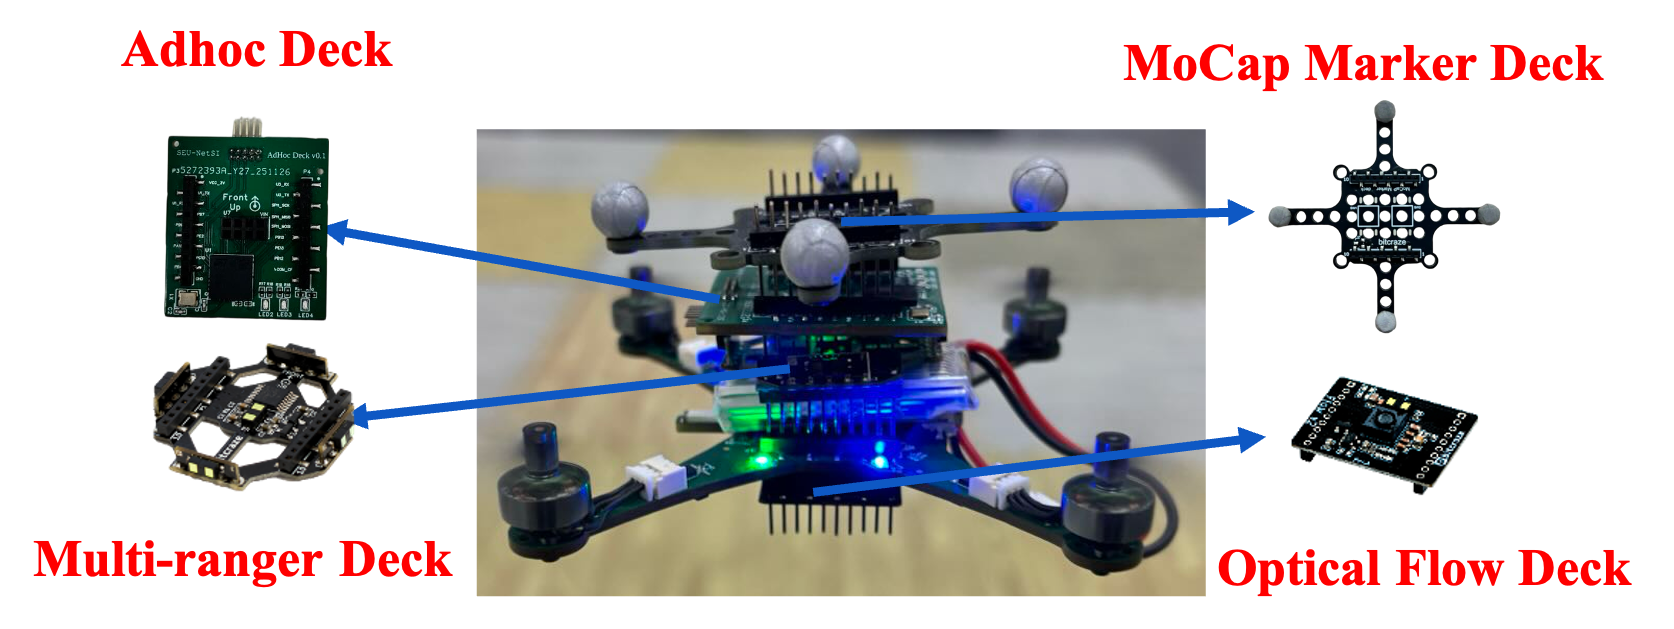
\includegraphics[width=.8\linewidth]{figures/content/chapter4/导航无人机.png}
  \caption{部署模型所用到的无人机及其扩展版}
  \label{fig:4_12}
\end{figure}

\begin{itemize}

  \item 嵌入式计算模块（Adhoc Deck）：作为模型推理的核心单元，搭载 Cortex-M7 处理器，负责执行压缩后的 IQN模型，实现实时路径决策与控制输出。
  
  \item 测距感知模块（Multi-ranger Deck）：由多个基于 ToF（Time-of-Flight）的激光测距传感器（VL53L1x）构成，分别安装于无人机前、后、左、右及上方方向，用于获取周围障碍物的距离信息，最终将数据传输至 Adhoc Deck，作为模型输入的一部分。
  
  \item 光流传感器模块（Optical Flow Deck）：由 VL53L1x 激光高度传感器和 PMW3901 光流传感器组成，可提供最高 100 Hz 的速度测量数据。
  
  \item 被动反光标记模块（MoCap Marker Deck）：由多个反光球组成，通过反射外部红外光源实现目标检测与识别，并由运动捕捉系统获取无人机的高精度位姿信息。
  
  \end{itemize}

  无人机真机导航任务在4.8×4.8米复杂环境中实施。如图\ref{fig:4_13}所示，在泡沫板场地中，我们在不同位置放置了形状大小各异的立方体作为我障碍物，并保证至少有一个障碍物在起点和终点的连线上，避免简单的直线飞行。

\begin{figure}[htbp]
  \centering
  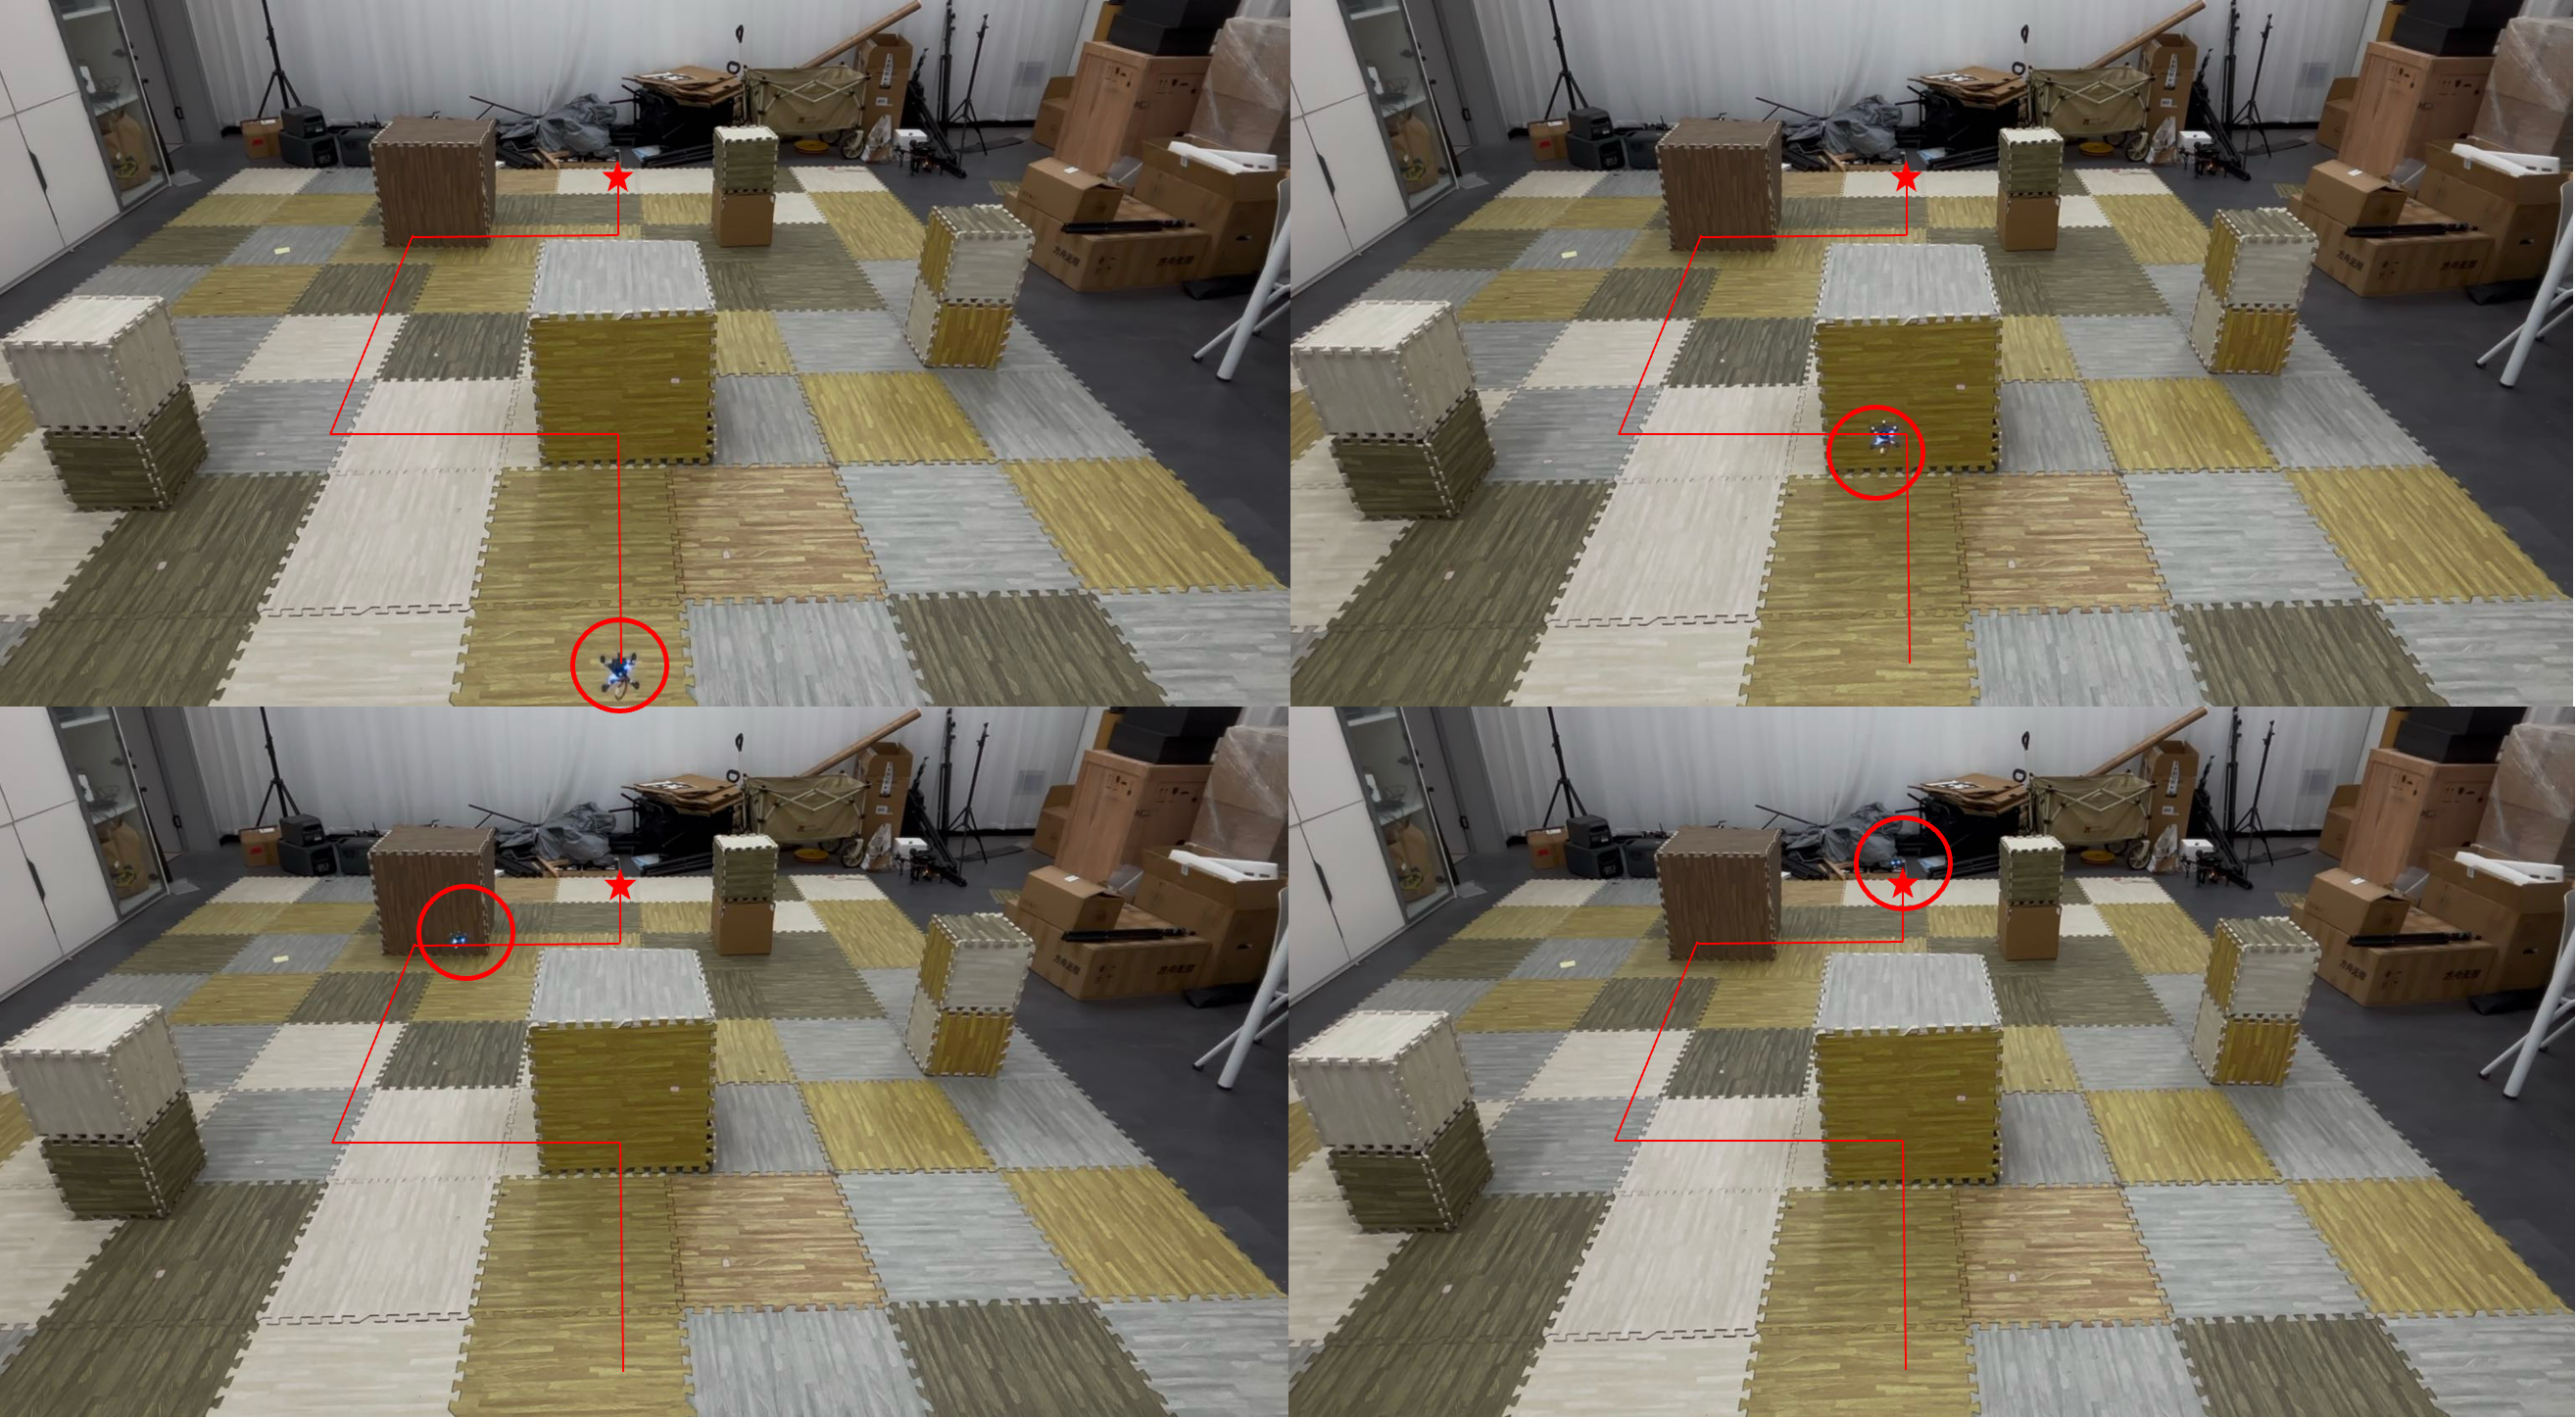
\includegraphics[width=.8\linewidth]{figures/content/chapter4/真机实验图.png}
    \caption{无人机自主导航实验图}
    \label{fig:4_13}
    \end{figure}

实验过程中，无人机需在未知环境中完成从起点到目标点的自主导航任务。
图\ref{fig:4_13}展示了实验过程中四个典型时刻的实拍图像，分别对应时刻1、时刻2、时刻3及时刻4。
在时刻2（图\ref{fig:4_13}(b)），无人机飞行至环境中第一个关键转折区域。面对局部障碍物或通道变化，导航系统实时更新路径规划策略，成功引导无人机调整航向，避免与周围环境发生碰撞。
最后，在时刻4（图\ref{fig:4_13}(d)），无人机成功抵达目标区域附近。此时，无人机已顺利完成导航任务，飞行轨迹收敛至目标点，整体导航过程平稳可靠。实验结果表明，本文方法能够在实际飞行条件下实现稳定、有效的自主导航。
\section{本章小结}

本章围绕无人机在复杂未知环境中的自主导航问题，系统地开展了从算法设计、模型训练到嵌入式部署与真机验证的完整研究工作。

首先，针对传统强化学习方法仅关注期望回报、难以应对低概率高风险事件的问题，本文在分布式强化学习框架下，引入回报分布建模思想，构建了基于隐式分位数网络的导航模型。在此基础上，提出了自适应风险倾向隐式分位网络算法，通过结合条件风险价值与回报分布特性，使智能体能够在决策过程中综合考虑收益与风险，从而提升在复杂环境中的安全性与鲁棒性。同时，引入右截断方差刻画内在不确定性，并基于其变化动态调整风险倾向，实现策略在风险规避与效率之间的自适应平衡。最后通过构建二维仿真环境并引入域随机化与渐进式训练策略，有效提升了模型的泛化能力。实验结果表明，相较于传统DQN及固定风险偏好的IQN方法，ART-IQN在成功率、碰撞率与导航效率等指标上均表现出更优的综合性能，验证了所提方法在复杂环境中的有效性。

在模型部署方面，针对嵌入式平台资源受限与实时性要求高的特点，本文基于STM32Cube.AI工具链对训练模型进行了量化、压缩。优化后的模型成功部署于Adhoc Deck扩展板，实现了端侧实时推理，并与Crazyflie 2.1无人机飞控系统协同工作，构建了“感知—决策—控制”的闭环自主导航系统。

最后，通过真实飞行实验对所提出方法进行了验证。实验结果表明，经过压缩优化后的模型能够在嵌入式硬件上稳定运行，并在实际复杂环境中实现有效避障与自主导航，具备良好的实时性与环境适应能力。


      % 第四章：
\chapter{微型无人机集群测距与自主导航原型系统}


\section{ 引言}

随着微型无人机在复杂环境中的应用需求不断提升，单机自主导航已难以满足高效率、高鲁棒性的任务要求，多无人机集群协同逐渐成为研究热点。
然而，在实际应用中，受限于微型无人机平台的计算资源、通信带宽以及传感能力，实现集群级别的稳定测距、可靠定位以及自主导航仍面临诸多挑战，尤其是在复杂未知环境下，如何构建一个具备完整闭环能力的原型系统，是从算法研究走向工程落地的关键问题。

针对上述问题，本文在前几章的研究基础上，进一步开展微型无人机集群测距与自主导航原型系统的设计与实现工作。
第三章围绕集群相对定位问题，提出了一种基于UWB的自适应协同定位方法，通过鲁棒测距协议与期望最大化算法相结合，实现了多无人机环境下稳定且高精度的相对定位；
第四章则针对复杂环境中的自主导航问题，基于分布式强化学习框架，提出了自适应风险倾向隐式分位网络算法，有效提升了无人机在低概率高风险场景下的决策安全性与鲁棒性，并完成了模型训练与嵌入式部署。

在此基础上，本章面向系统级集成与真实场景验证，构建了一个完整的微型无人机集群自主导航原型系统。
该系统以Crazyflie 2.1微型无人机为核心平台，结合Adhoc Deck扩展板，实现机载计算、通信与感知能力的集成。
在系统架构上，采用“感知—定位—决策—控制”的分层设计思路，其中领导者无人机基于第四章提出的导航算法实现自主路径规划与避障飞行，而跟随无人机则依托第三章的协同定位方法获取相对位姿信息，并结合简化避障策略完成编队跟随与局部避碰，从而实现集群层面的协同运动。

同时，为保证系统在实际运行中的稳定性与实时性，本文进一步设计并实现了完整的软硬件体系，包括嵌入式模型部署、无人机内部通信机制、飞行控制接口以及外部监控系统等关键模块，并对系统运行流程与部署方案进行了系统化设计。
通过构建真实飞行实验环境，对所提出的集群测距与自主导航方法进行了综合验证。

实验结果表明，所构建的原型系统能够在资源受限的微型无人机平台上稳定运行，实现多无人机之间的可靠测距与协同定位，并支持领航-跟随模式下的自主导航与避障飞行，验证了本文所提方法在实际复杂环境中的可行性与有效性。

\section{系统硬件组成}
\begin{figure}[htbp]
  \centering
  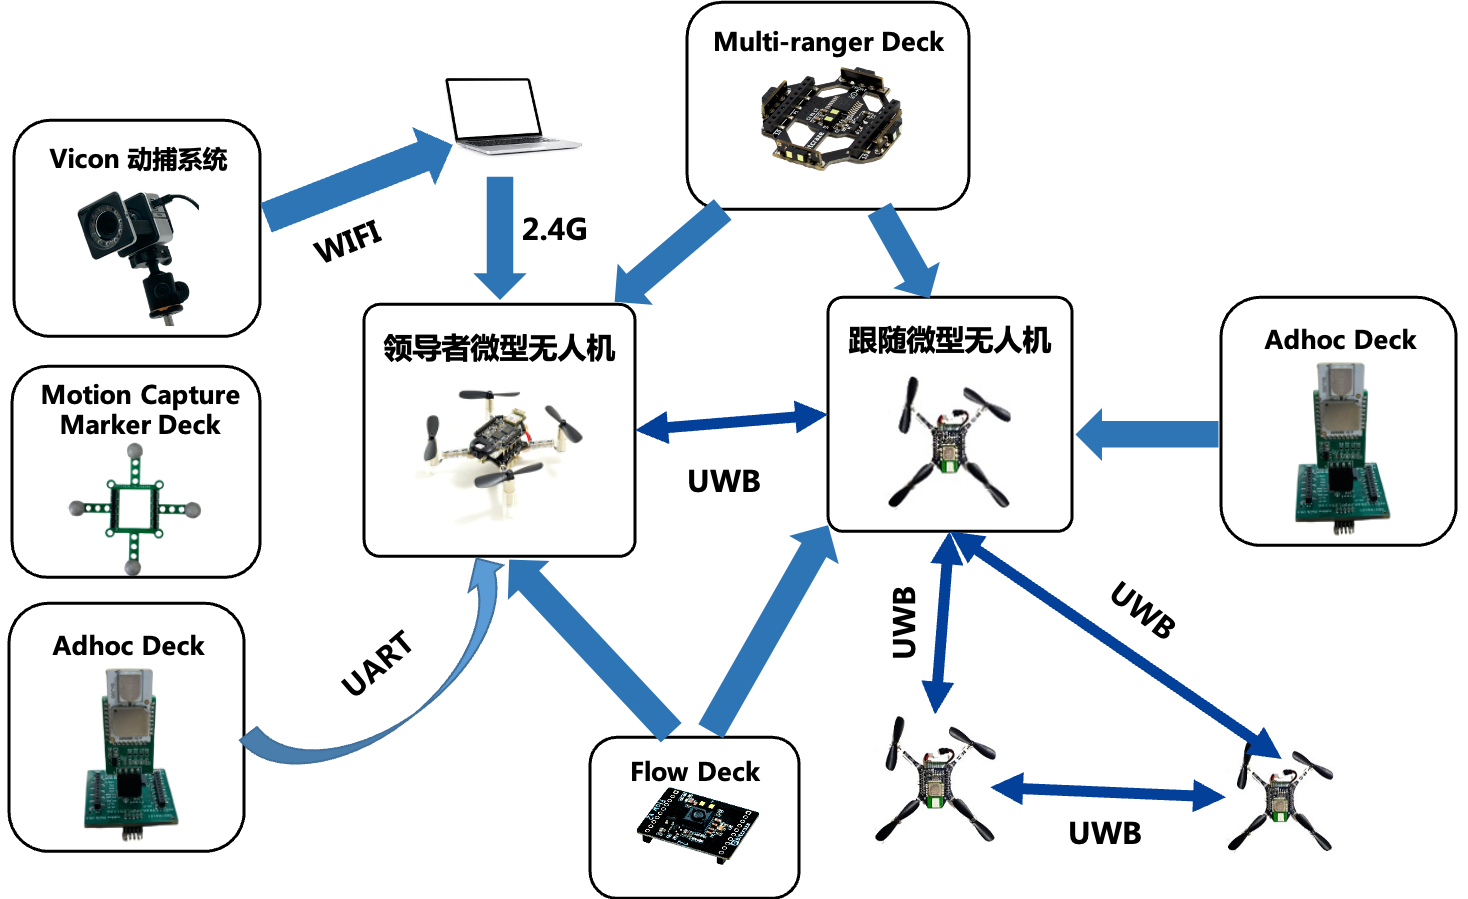
\includegraphics[width=.8\linewidth]{figures/content/chapter5/硬件架构.png}
  \caption{原型系统硬件架构}
  \label{fig:5_1}
\end{figure}

本文构建的微型无人机集群自主导航系统的硬件架构如图\ref{fig:5_1}，整体由外部监控系统、领导者无人机、跟随者无人机以及多种计算或传感器扩展模块组成。

在外部系统部分，基于 Vicon 动作捕捉系统 与 Motion Capture Marker Deck 实现高精度位姿获取，并通过服务器经 WiFi 将位置信息发送至电脑端。
同时，电脑端通过Crazy Radio PA的2.4GHz 无线链路与无人机通信，作为导航传入的必要数据。

在无人机平台方面，系统采用“领导者—跟随者”分层结构：领导者无人机搭载 Adhoc Deck 与 其他的传感器扩展模块，其中 Adhoc Deck 提供嵌入式计算能力与UWB通信，用于运行协同定位算法与自主导航；
其他的传感器模块用来为导航传入必要的输入数据。
跟随无人机主要依赖 UWB 模块进行相对测距与定位，通过与领导者及其他无人机之间的 UWB 通信，实现分布式协同定位与编队跟随。
\subsection{无人机平台}
\begin{figure}[htbp]
    \centering
    \subfloat[Adhoc Deck]{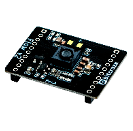
\includegraphics[width=.23\textwidth]{figures/content/chapter5/FlowDeck.png}}
    \quad
    \subfloat[Flow Deck]{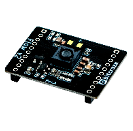
\includegraphics[width=.23\textwidth]{figures/content/chapter5/FlowDeck.png}}
    \quad
    \subfloat[Multi-ranger Deck]{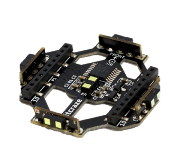
\includegraphics[width=.23\textwidth]{figures/content/chapter5/MultirangDeck.png}}
    \quad
    \subfloat[Motion Capture Marker Deck]{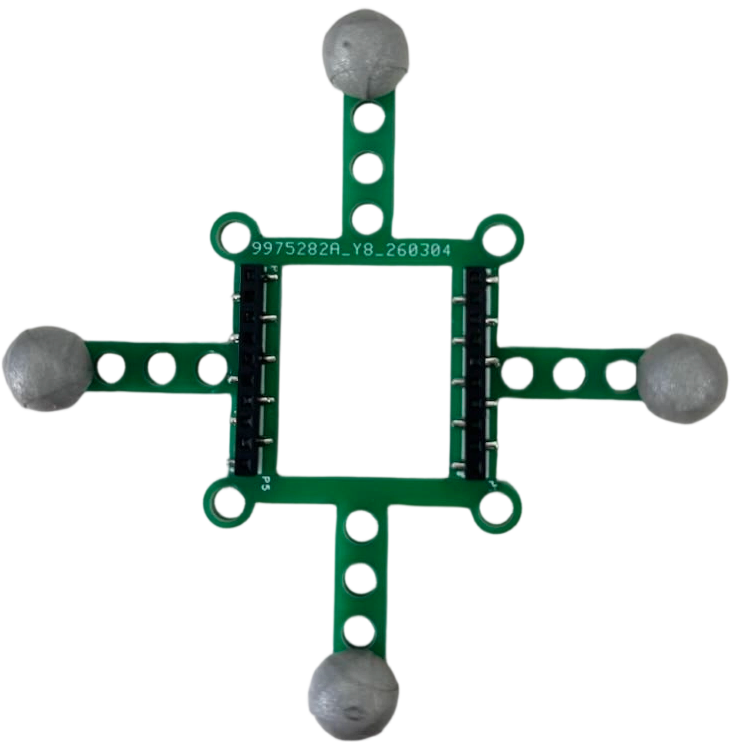
\includegraphics[width=.23\textwidth]{figures/content/chapter5/viconDeck.png}}
    \caption{领导者无人机硬件模块组成}
    \label{fig:5_2}
    \end{figure}
如图\ref{fig:5_2}所示，领岛无人机搭载了多种功能扩展板，用于实现感知、计算与定位等关键功能，具体包括 Adhoc Deck、Flow Deck、Multi-ranger Deck 以及 Motion Capture Marker Deck。

其中，Adhoc Deck 是系统的核心计算模块，基于嵌入式处理器构建，负责运行本文提出的协同自主定位于自主导航算法，实现机载实时决策。
同时，该扩展板支持外设接口扩展，可集成 UWB 模块，从而具备测距与通信能力，使领导者无人机既能够执行导航任务，又能够参与集群间的相对定位与信息交互。
Flow Deck 主要用于提供对地速度与高度信息，其通过光流传感器与 ToF 距离传感器实现对无人机平面运动速度及离地高度的估计，在无外部定位系统的情况下可辅助飞行稳定与状态估计。
Multi-ranger Deck 集成多个方向的距离传感器，可实时获取无人机前、后、左、右及上方的障碍物距离信息，为自主导航算法提供环境感知输入，从而支持局部避障决策。
Motion Capture Marker Deck 搭载反光标记点，用于配合外部动捕系统获取高精度位姿信息，为导航模型提供输入的数据。


\begin{figure}[htbp]
    \centering
    \subfloat[UWB Deck]{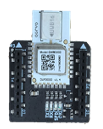
\includegraphics[width=.23\textwidth]{figures/content/chapter5/UWBDeck.png}}
    \quad
    \subfloat[Flow Deck]{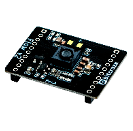
\includegraphics[width=.33\textwidth]{figures/content/chapter5/FlowDeck.png}}
    \quad
    \subfloat[Multi-ranger Deck]{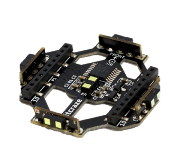
\includegraphics[width=.33\textwidth]{figures/content/chapter5/MultirangDeck.png}}
    \caption{跟随者无人机硬件模块组成}
    \label{fig:5_3}
    \end{figure}
如图\ref{fig:5_3}所示，跟随无人机主要搭载 UWB Deck、Flow Deck 以及 Multi-ranger Deck，以实现相对定位与局部避障等功能。

其中，UWB Deck 是跟随无人机实现协同定位的核心模块。该扩展板基于 UWB 芯片，能够与领导无人机及其他跟随者之间进行高精度测距与数据交互。通过构建多节点间的测距网络，并结合第三章提出的自适应协同定位算法，跟随无人机能够实时获取自身在集群中的相对位姿信息，从而实现对领导者的稳定跟随。
Multi-ranger Deck 集成多方向距离传感器，用于实时感知周围障碍物距离信息。
跟随无人机在执行编队跟随任务的同时，可基于该模块提供的环境感知信息实现局部避障与避碰，从而提升系统在复杂环境中的安全性。

领导者与跟随者无人机搭载各种扩展版的最终图\ref{fig:5_4}所示。
\begin{figure}[htbp]
    \centering
    \subfloat[领导者无人机]{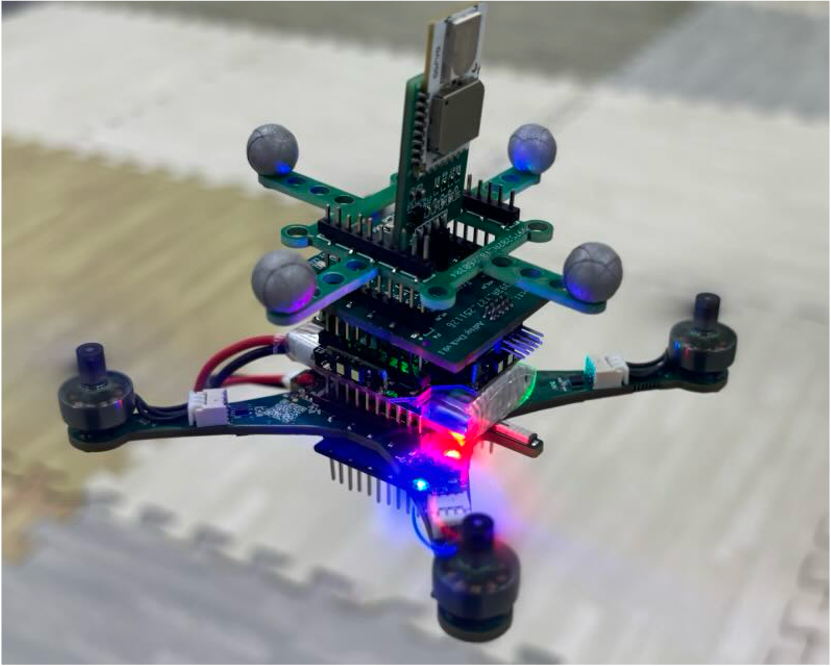
\includegraphics[width=.45\textwidth]{figures/content/chapter5/领导者图片.png}}
    \quad
    \subfloat[跟随者无人机]{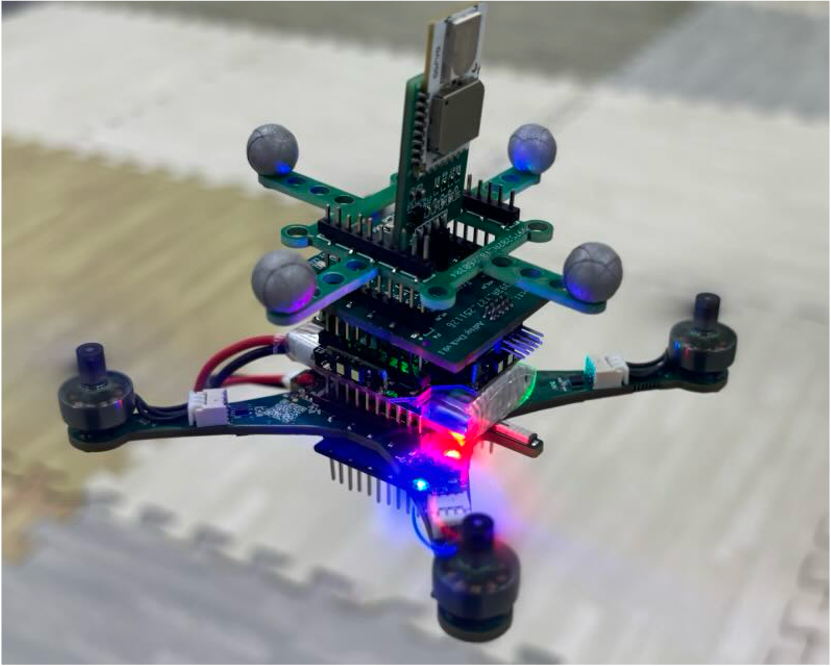
\includegraphics[width=.45\textwidth]{figures/content/chapter5/领导者图片.png}}
    \caption{无人机集群自主导航系统}
    \label{fig:5_3}
\end{figure}
\subsection{外部监控平台}
外部监控平台主要由 Vicon 动作捕捉系统 与 Crazyradio PA 无线通信模块 构成，用于实现无人机状态获取与飞行指令下发。

\begin{figure}[htbp]
  \centering
  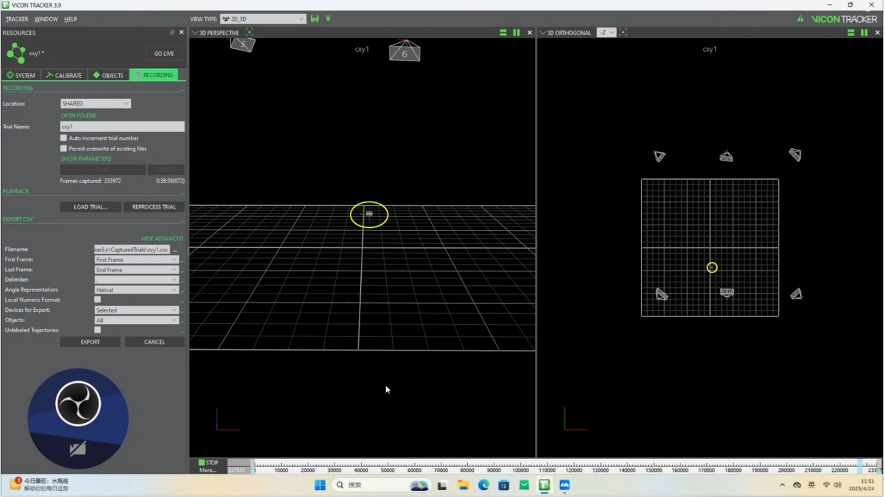
\includegraphics[width=.7\linewidth]{figures/content/chapter5/vicon平台.png}
  \caption{vicon 监控平台}
  \label{fig:5_4}
\end{figure}

其中，Vicon 动作捕捉系统 通过在无人机上安装 Motion Capture Marker Deck，利用多台红外摄像机对标记点进行实时捕捉与三维重建，从而获取无人机在全局坐标系下的高精度位姿信息。该系统具有厘米级甚至毫米级的定位精度与较高的更新频率，可为算法开发与实验验证提供可靠的“真值”参考。

在安装 Motion Capture Marker Deck 后，需要对动作捕捉系统进行校准，以确保定位精度与系统稳定性。具体步骤如下：

\begin{enumerate}
    \item 准备工作：  
    确保 Vicon 系统硬件（如摄像机、反光标记球等）已正确安装并连接正常，相关软件已完成安装并成功启动。同时，将反光球合理粘贴在被捕捉对象（如人体或无人机）关键位置，以保证后续识别的稳定性与准确性。

    \item 摄像机聚焦：  
    打开 Vicon 系统软件，进入摄像机调试与聚焦模块。按照软件提示依次对各个摄像机进行校准，使各摄像机视野中不存在多余光斑（建议在避光环境下进行）。当每个摄像机画面中的标记点均显示为蓝色时，表明摄像机校准完成。

    \item 空间坐标校准：  
    使用校准工具（带反光球的标定棒）在整个捕捉空间内移动，构建全局空间坐标系。系统根据多摄像机采集的数据，计算空间中各标记点的位置关系，从而完成对捕捉空间范围及坐标系的标定。

    \item 建立刚体模型：  
    检查粘贴在 Motion Capture Marker Deck 上的反光球是否牢固且分布合理。将无人机置于捕捉空间内，系统对反光球的标记点进行识别与建模。通常至少需要三个非共线标记点才能建立刚体模型，本实验中共使用四个反光球进行建模，最终建立的刚体模型如图~\ref{fig:5_4} 所示。

    \item 数据检查：  
    校准完成后，进行简单的动作捕捉测试，观察系统输出的数据是否连续、平滑，是否存在异常跳变或数据丢失现象。如发现问题，应返回对应步骤重新进行校准，以确保系统性能满足实验要求。
\end{enumerate}

Crazyradio PA 是用于连接上位机与无人机的 2.4GHz 无线通信模块。其通过 USB 接口与计算机相连，并基于 Crazyflie 通信协议（CRTP）与无人机建立稳定的数据链路。
上位机可通过 Crazyradio PA 向领导者无人机发送飞行控制指令，同时接收无人机回传的状态信息，实现对系统运行过程的实时监控与参数调节。

\section{系统软件模块}
本文构建的微型无人机集群测距与自主导航原型系统在软件层面采用分层解耦与模块化设计方法，整体由单机功能模块、集群协同功能模块以及算法支撑模块三部分组成，并围绕“感知—定位—决策—控制—通信”的处理流程构建完整闭环。

在单机层面，系统根据功能角色的不同，将无人机划分为领导者与跟随者两类节点，其软件架构在统一框架下进行差异化设计。

对于领导者无人机，其模块层主要包括飞行控制模块、自主导航模块以及协同定位模块。其中，飞行控制模块位于系统底层，负责接收上层控制指令并完成姿态与速度的闭环控制；自主导航模块作为核心决策单元，基于强化学习模型输出无人机在复杂环境中的运动决策，实现路径规划与动态避障；协同定位模块则参与集群测距与状态估计过程，为系统提供相对位置信息支撑。各模块之间通过统一的数据接口进行交互，使导航决策能够平滑映射至底层控制执行。

对于跟随无人机，其模块层包括飞行控制模块、协作通信定位模块以及局部避障模块。其中，协作通信定位模块基于 UWB 测距与信息交互机制，结合分布式定位算法实现无人机间的相对位姿估计；局部避障模块利用机载传感器信息对周围环境进行感知，并在跟随过程中对潜在碰撞进行规避；飞行控制模块则根据定位结果与跟随策略输出控制量，实现对领导者无人机的稳定跟随。相比领导者，跟随者不直接参与全局路径规划，而侧重于协同感知与局部决策。

在集群层面，系统进一步抽象为两个核心子系统，即集群定位飞行任务子系统与自主导航任务子系统。其中，集群定位飞行任务子系统主要负责无人机之间的测距、通信以及协同定位，对应本文第三章提出的自适应协同定位方法；自主导航任务子系统则由领导无人机主导，负责在复杂未知环境中的路径规划与避障决策，对应第四章提出的强化学习导航算法。两个子系统相互协同，共同支撑集群飞行任务的完成。

在数据流层面，系统整体运行过程可描述为：环境感知与测距数据首先由各类传感器与通信模块获取，经协同定位模块融合得到无人机状态信息；
随后，领导者无人机基于自主导航模块输出控制决策，跟随无人机根据相对位姿与跟随策略生成控制指令；最终，飞行控制模块将高层指令转换为底层执行信号，驱动无人机完成相应运动。同时，通信模块贯穿整个系统，实现无人机之间以及无人机与上位机之间的数据交互。
在上述整体架构基础上，针对前文尚未详细说明的关键功能模块，本文进一步对跟随避障算法、通信模块以及飞行控制模块进行补充说明。
\begin{figure}[htbp]
  \centering
  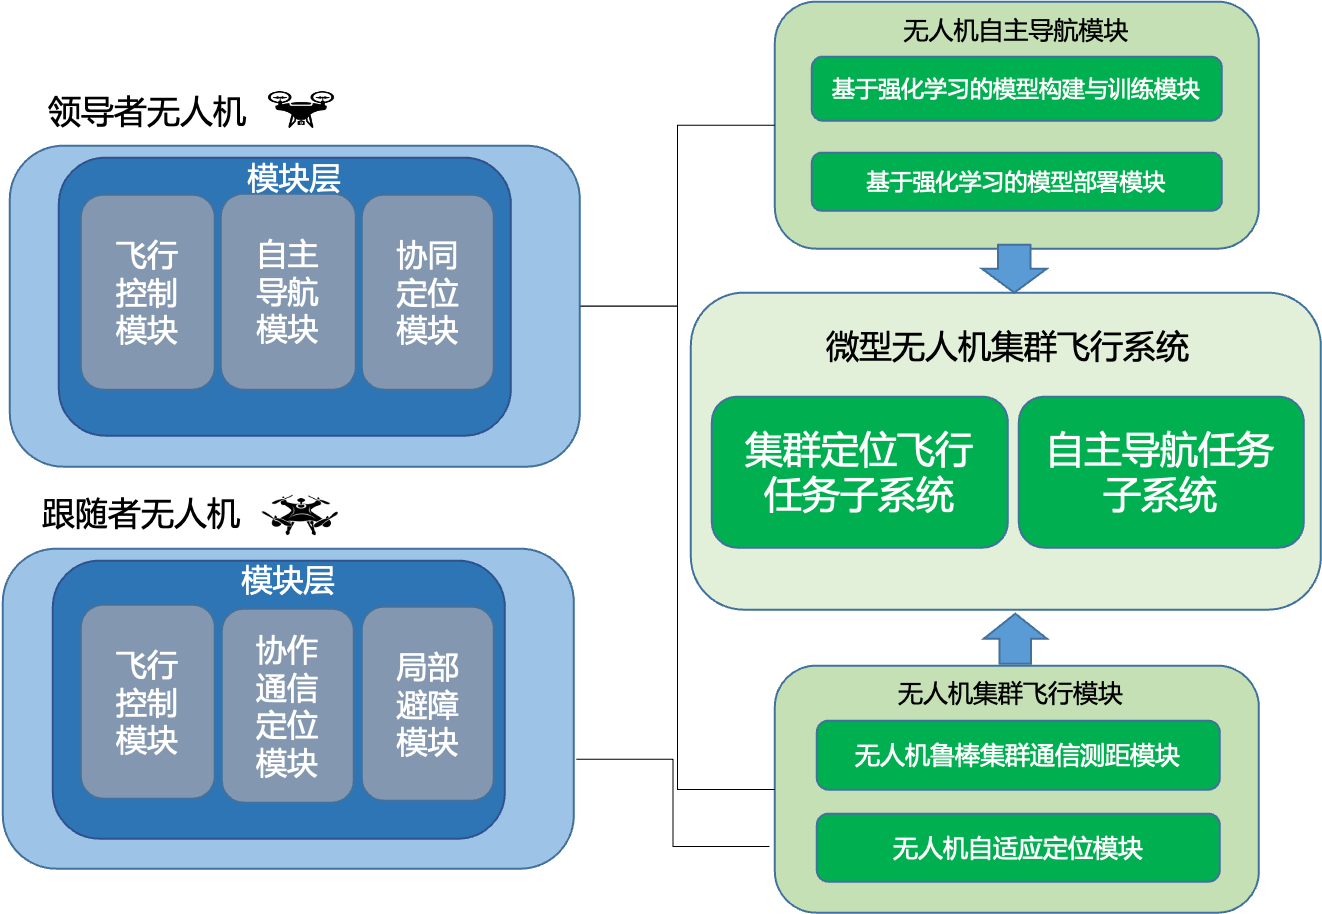
\includegraphics[width=.6\linewidth]{figures/content/chapter5/软件架构.png}
  \caption{系统软件架构}
  \label{fig:5_5}
\end{figure}
\subsection{跟随与避障模块}
在多无人机编队飞行中，每架无人机都有其在领导者坐标系下的预定位置。
为了简化问题，我们将0号无人机设置为编队中的领导者，因此其预定位置被设为坐标系原点。
首先，仅考虑编队保持任务时，第$i$架无人机的速度控制律采用经典PID形式\cite{knospe2006pid}表示为：
\begin{equation}
\boldsymbol{v}_{i}=k_{p} \boldsymbol{e}_{i 0}+k_{d} \dot{\boldsymbol{e}}_{i 0}+k_{i} \int \boldsymbol{e}_{i 0} d t
\end{equation}
其中，$\boldsymbol{e}_{i 0}$为领导者与跟随着的相对位置偏差，也就是预定位置和实际位置之间的差异。

对于无人机周边的外界障碍物的碰撞避免，我们假设无人机可以通过传感器得知障碍物相对机体坐标系下的具体位置$ \boldsymbol{p}_{i}^{o b s}=\left(x_{i}^{o b s}, y_{i}^{o b s}\right)$和距离机体的距离$d_{i}^{o b s}$。
当无人机靠近障碍物$c$米时开始产生阻碍速度，阻碍增益系数为$k_{o b s}$。
当无人机靠近障碍物时，我们增高相应的排斥速度，以避免碰撞发生。
因此，我们设计了一个具有防止无人机与障碍物发生碰撞的编队控制协议。
\begin{equation}
\boldsymbol{v}_{i}=k_{p} \boldsymbol{e}_{i 0}+k_{d} \dot{\boldsymbol{e}}_{i 0}+k_{i} \int \boldsymbol{e}_{i 0} d t-\sum_{j}^{N_{o b s}} k_{o b s}\left(c-\min \left(d_{j}^{o b s}, c\right)\right) \operatorname{sign}\left(\boldsymbol{p}_{j}^{o b s}\right)^{\circ}\left|\boldsymbol{p}_{j}^{o b s}\right|^{-1}
\end{equation}
\subsection{通信模块}
在本文系统中，无人机与上位机之间的通信采用 Crazyflie 平台提供的 Crazy Real-Time Protocol（CRTP） 协议实现。CRTP 是一种轻量级、面向实时控制设计的数据通信协议，主要用于在上位机与无人机各功能子系统之间进行高效、可靠的数据交互。

从体系结构上看，CRTP 采用分层设计，其通信栈自下而上包括物理层、链路层、协议层以及功能子系统层。其中，物理层支持 USB 或 2.4GHz 无线链路（Crazyradio PA）；链路层负责数据包的可靠传输与顺序控制；CRTP 协议层通过引入端口（port）与通道（channel）机制，实现数据在不同功能模块之间的路由；最上层的子系统则对应无人机内部的具体功能模块，如飞行控制、参数管理、数据日志与定位等。

在数据结构方面，每个 CRTP 数据包由端口号、通道号以及负载数据组成。其中，端口号占 4 位（范围 0–15），用于标识目标功能模块；通道号占 2 位（范围 0–3），用于模块内部功能区分；负载数据最大为 30 字节。该设计使得协议具有较低开销，同时能够灵活支持多模块并行通信。

Adhoc Deck 与无人机之间基于 UART进行数据通信。
该部分主要负责两者之间的指令交互与状态数据传输，是支撑上层协同算法与控制逻辑运行的关键基础。
在具体实现上，通信链路基于 STM32H7 平台的 UART 外设构建，并结合 DMA 机制实现高效的数据收发，以降低 CPU 占用率。同时，引入 UART 空闲中断用于检测数据帧边界，从而支持变长数据的可靠接收。在发送方向，通过数据组包与二值信号量相结合的方式，对 DMA 发送过程进行同步控制，避免多任务环境下的资源冲突；在接收方向，采用“DMA 接收 + IDLE 中断触发 + 回调处理”的流程，将接收到的字节流进行解析并写入线程安全的环形队列，供应用层按需读取。

在此基础上，本文进一步对通信模块的具体实现机制进行设计与分析，重点介绍系统初始化流程、数据收发机制以及软件分层结构。

无人机上电后，系统首先完成 BSP 层与 Module 层的初始化工作。关键初始化过程包括：创建用于数据接收的环形队列、初始化用于发送同步的二值信号量 tx\_semaphore（初始为空闲状态），以及注册底层接收回调函数 receive\_callback，为后续通信流程的稳定运行奠定基础。

在通信机制设计方面，系统分别对发送链路（TX Flow）与接收链路（RX Flow）进行了优化设计。对于发送链路，采用“数据组包 → 等待二值信号量（确保上一轮 DMA 传输完成）→ 启动新一轮 DMA 发送”的处理流程，通过信号量机制实现对 DMA 资源的互斥访问，从而避免多任务环境下的发送冲突，并保证数据传输的时序正确性与完整性。

对于接收链路，系统采用“DMA 硬件接收 → UART 空闲中断（IDLE）触发 → 调用接收回调函数 → 数据解包并写入环形队列 → 应用层读取”的处理流程。其中，利用 UART 空闲中断对变长数据帧进行边界检测，有效提升了数据接收的灵活性与效率。在中断回调函数中，为确保环形队列在中断上下文中的操作安全性，采用 FreeRTOS 提供的 taskENTER\_CRITICAL\_FROM\_ISR() 机制对队列读写指针进行保护，从而避免中断嵌套或任务抢占导致的数据一致性问题。

从系统架构角度出发，Adhoc Deck 与无人机主控之间的通信模块采用分层设计思想，可划分为以下三个层次：


\begin{itemize}
    \item 硬件驱动层（bsp\_transmit.c/h）
    该层负责 STM32H7 底层外设（如 UART3 与 DMA1）的初始化与配置，管理发送与接收缓冲区，并实现基于“DMA + UART 空闲中断（IDLE）”的变长数据帧接收机制，为上层提供高效、低开销的数据传输接口。

    \item 协议解析层（transmit\_packet.c/h, transmit\_config.h）
    该层定义通信数据包的结构与消息类型，负责原始字节流的封包与解包处理，并维护线程安全的环形接收队列，实现中断上下文与任务上下文之间的数据解耦与可靠传递。

    \item 系统与中断管理层（stm32h7xx\_it.c, main.c）  
    该层负责中断向量的统一管理（包括 UART3 空闲中断与 DMA 传输完成中断），并通过 \texttt{USER\_INIT} 宏机制实现各功能模块的自动注册与初始化，从而提高系统的模块化程度与可维护性。
\end{itemize}

\begin{lstlisting}[language=C, caption={通信数据包结构定义}]
typedef struct __attribute__((packed)){
    uint8_t header;                   // 帧头 (0xAA)
    Transmit_Packet_Type_t msg_type;  // 消息类型
    uint8_t data_len;                 // 有效载荷长度
    uint8_t data[MAX_PAYLOAD_SIZE];   // 有效载荷数据
} Transmit_Packet_t;
\end{lstlisting}
此外，为降低通信开销并提升跨平台兼容性，通信数据包采用紧凑的数据结构设计，通过显式控制内存布局以消除编译器默认对齐带来的冗余填充，从而在保证数据一致性与可解析性的同时，提高整体通信效率。
\subsection{飞行控制模块}
\begin{figure}[htbp]
  \centering
  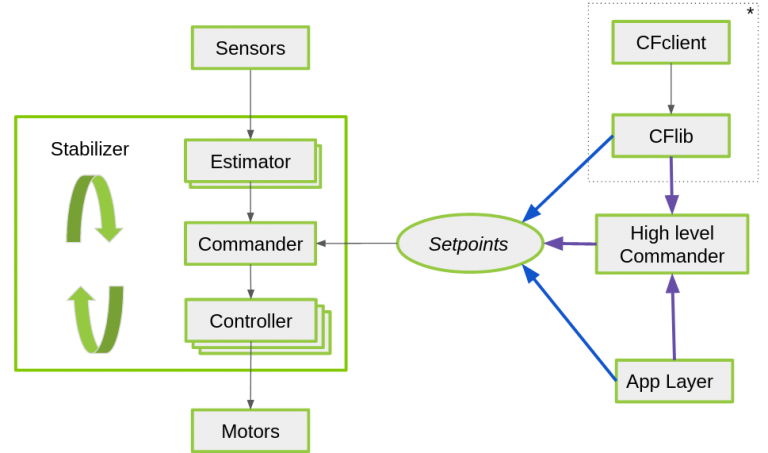
\includegraphics[width=.6\linewidth]{figures/content/chapter5/无人机飞控.png}
  \caption{无人机飞行控制的Commander模块}
  \label{fig:5_6}
  \end{figure}
Crazyflie 2.1 无人机的飞行控制模块采用基于 setpoint 的分层闭环控制架构，通过统一的目标状态描述实现上层控制输入与底层控制器之间的解耦。在该机制中，setpoint 用于描述无人机在当前时刻的期望状态，并作为控制器的参考输入，与状态估计模块输出的实际状态进行比较，从而驱动多层控制器逐级完成闭环调节。根据控制目标的不同，系统支持多种 setpoint 工作模式，包括绝对位置模式（modeAbs）、速度模式（modeVelocity）以及禁用模式（modeDisable），从而能够适应不同任务场景下的控制需求。

在本文的系统实现中，主要采用速度模式（modeVelocity）作为无人机的控制方式。在该模式下，setpoint 不再直接描述无人机的空间位置，而是以速度作为控制目标，具体包括$x$、$y$、$z$三个方向的线速度以及偏航角变化率。控制系统通过将期望速度与当前估计速度进行比较，构建速度闭环控制，并进一步生成对应的加速度指令。由于四旋翼无人机的平动控制依赖于姿态调节，系统将期望加速度转换为相应的滚转角与俯仰角设定值，随后通过姿态控制环和角速度控制环逐级实现闭环调节，最终作用于电机驱动，实现对无人机运动状态的精确控制。

相较于绝对位置模式，速度模式具有更加连续和平滑的控制特性。由于其不依赖离散的位置目标点，而是通过连续速度输入驱动无人机运动，因此能够有效避免位置控制中可能出现的震荡与突变问题。此外，速度模式对系统响应速度要求较低，控制链路更为直接，有利于提高动态响应性能。在多无人机协同控制或基于外部感知（如UWB定位）的场景中，通过直接控制速度可以更方便地实现一致性控制与分布式决策，因此具有更强的适用性。



在本系统中，H7 芯片上运行的飞行控制算法需要将控制指令（setpoint）实时传输至无人机固件执行。由于无线通信带宽受限，若每次均传输完整的 setpoint 结构体，将带来较大的通信开销。
因此，有必要对传输数据格式进行优化设计，以降低数据量并提升通信效率。

首先，通过对飞控过程中 setpoint 使用情况的分析发现，相较于默认值，每一时刻仅有部分字段发生变化。据此，本文提出一种基于“差分传输”的数据压缩方法，仅传输相对于默认 setpoint 的变化量，从而显著减少通信负载。

具体而言，设计如下差分数据结构：
\begin{lstlisting}[language=C]
struct Diff
{
    uint8_t change;
    uint8_t data[2 * SIZE_OF_SETPOINT];
};
\end{lstlisting}

其中，\texttt{change} 表示当前 setpoint 中相较默认值发生变化的字节数量；\texttt{data} 用于存储具体变化信息。对于每一个发生变化的字节，采用“位置 + 数值”的编码方式进行存储，即：
\begin{itemize}
    \item \texttt{data[2n]} 表示发生变化的字节在 setpoint 中的位置索引；
    \item \texttt{data[2n+1]} 表示该位置更新后的数值。
\end{itemize}

因此，在实际传输过程中，仅需发送 $2 \times \texttt{change} + 1$ 个字节即可完成一次 setpoint 更新，相较于原始整结构体传输方式大幅降低了数据量。

在接收端，无人机固件首先加载默认 setpoint，然后根据接收到的差分数据，对对应位置进行逐字节更新，从而恢复出完整的控制指令。

为验证该方法的有效性，本文在无人机固件中构建了“自发送”测试机制，即由系统内部模拟 H7 芯片发送飞控数据。实验结果表明，该方法能够在保证飞行控制正常执行的前提下显著降低通信开销。在一次典型飞行测试中，改进方案的数据传输总量约为原始方案的 $15.58\%$，验证了所提出方法的高效性与可行性。

\section{系统部署与运行方案}
在系统部署过程中，不同模块采用了不同的程序烧录与调试方式。对于 Crazyflie 无人机本体，其固件通过 Crazyradio PA 无线模块进行烧录，上位机经由 2.4GHz 通信链路将编译好的固件下载至无人机，实现快速更新与部署。

对于 Adhoc Deck 扩展板，其程序烧录采用 ST-Link 调试器，通过 SWD 接口将程序下载至 STM32H7 芯片中。该方式主要用于嵌入式算法与底层驱动的开发与调试。

在调试方面，Adhoc Deck 采用 SWV（Serial Wire Viewer）机制进行运行信息输出，通过调试接口实时打印关键变量与系统状态，用于辅助程序调试与功能验证。

\begin{figure}[htbp]
  \centering
  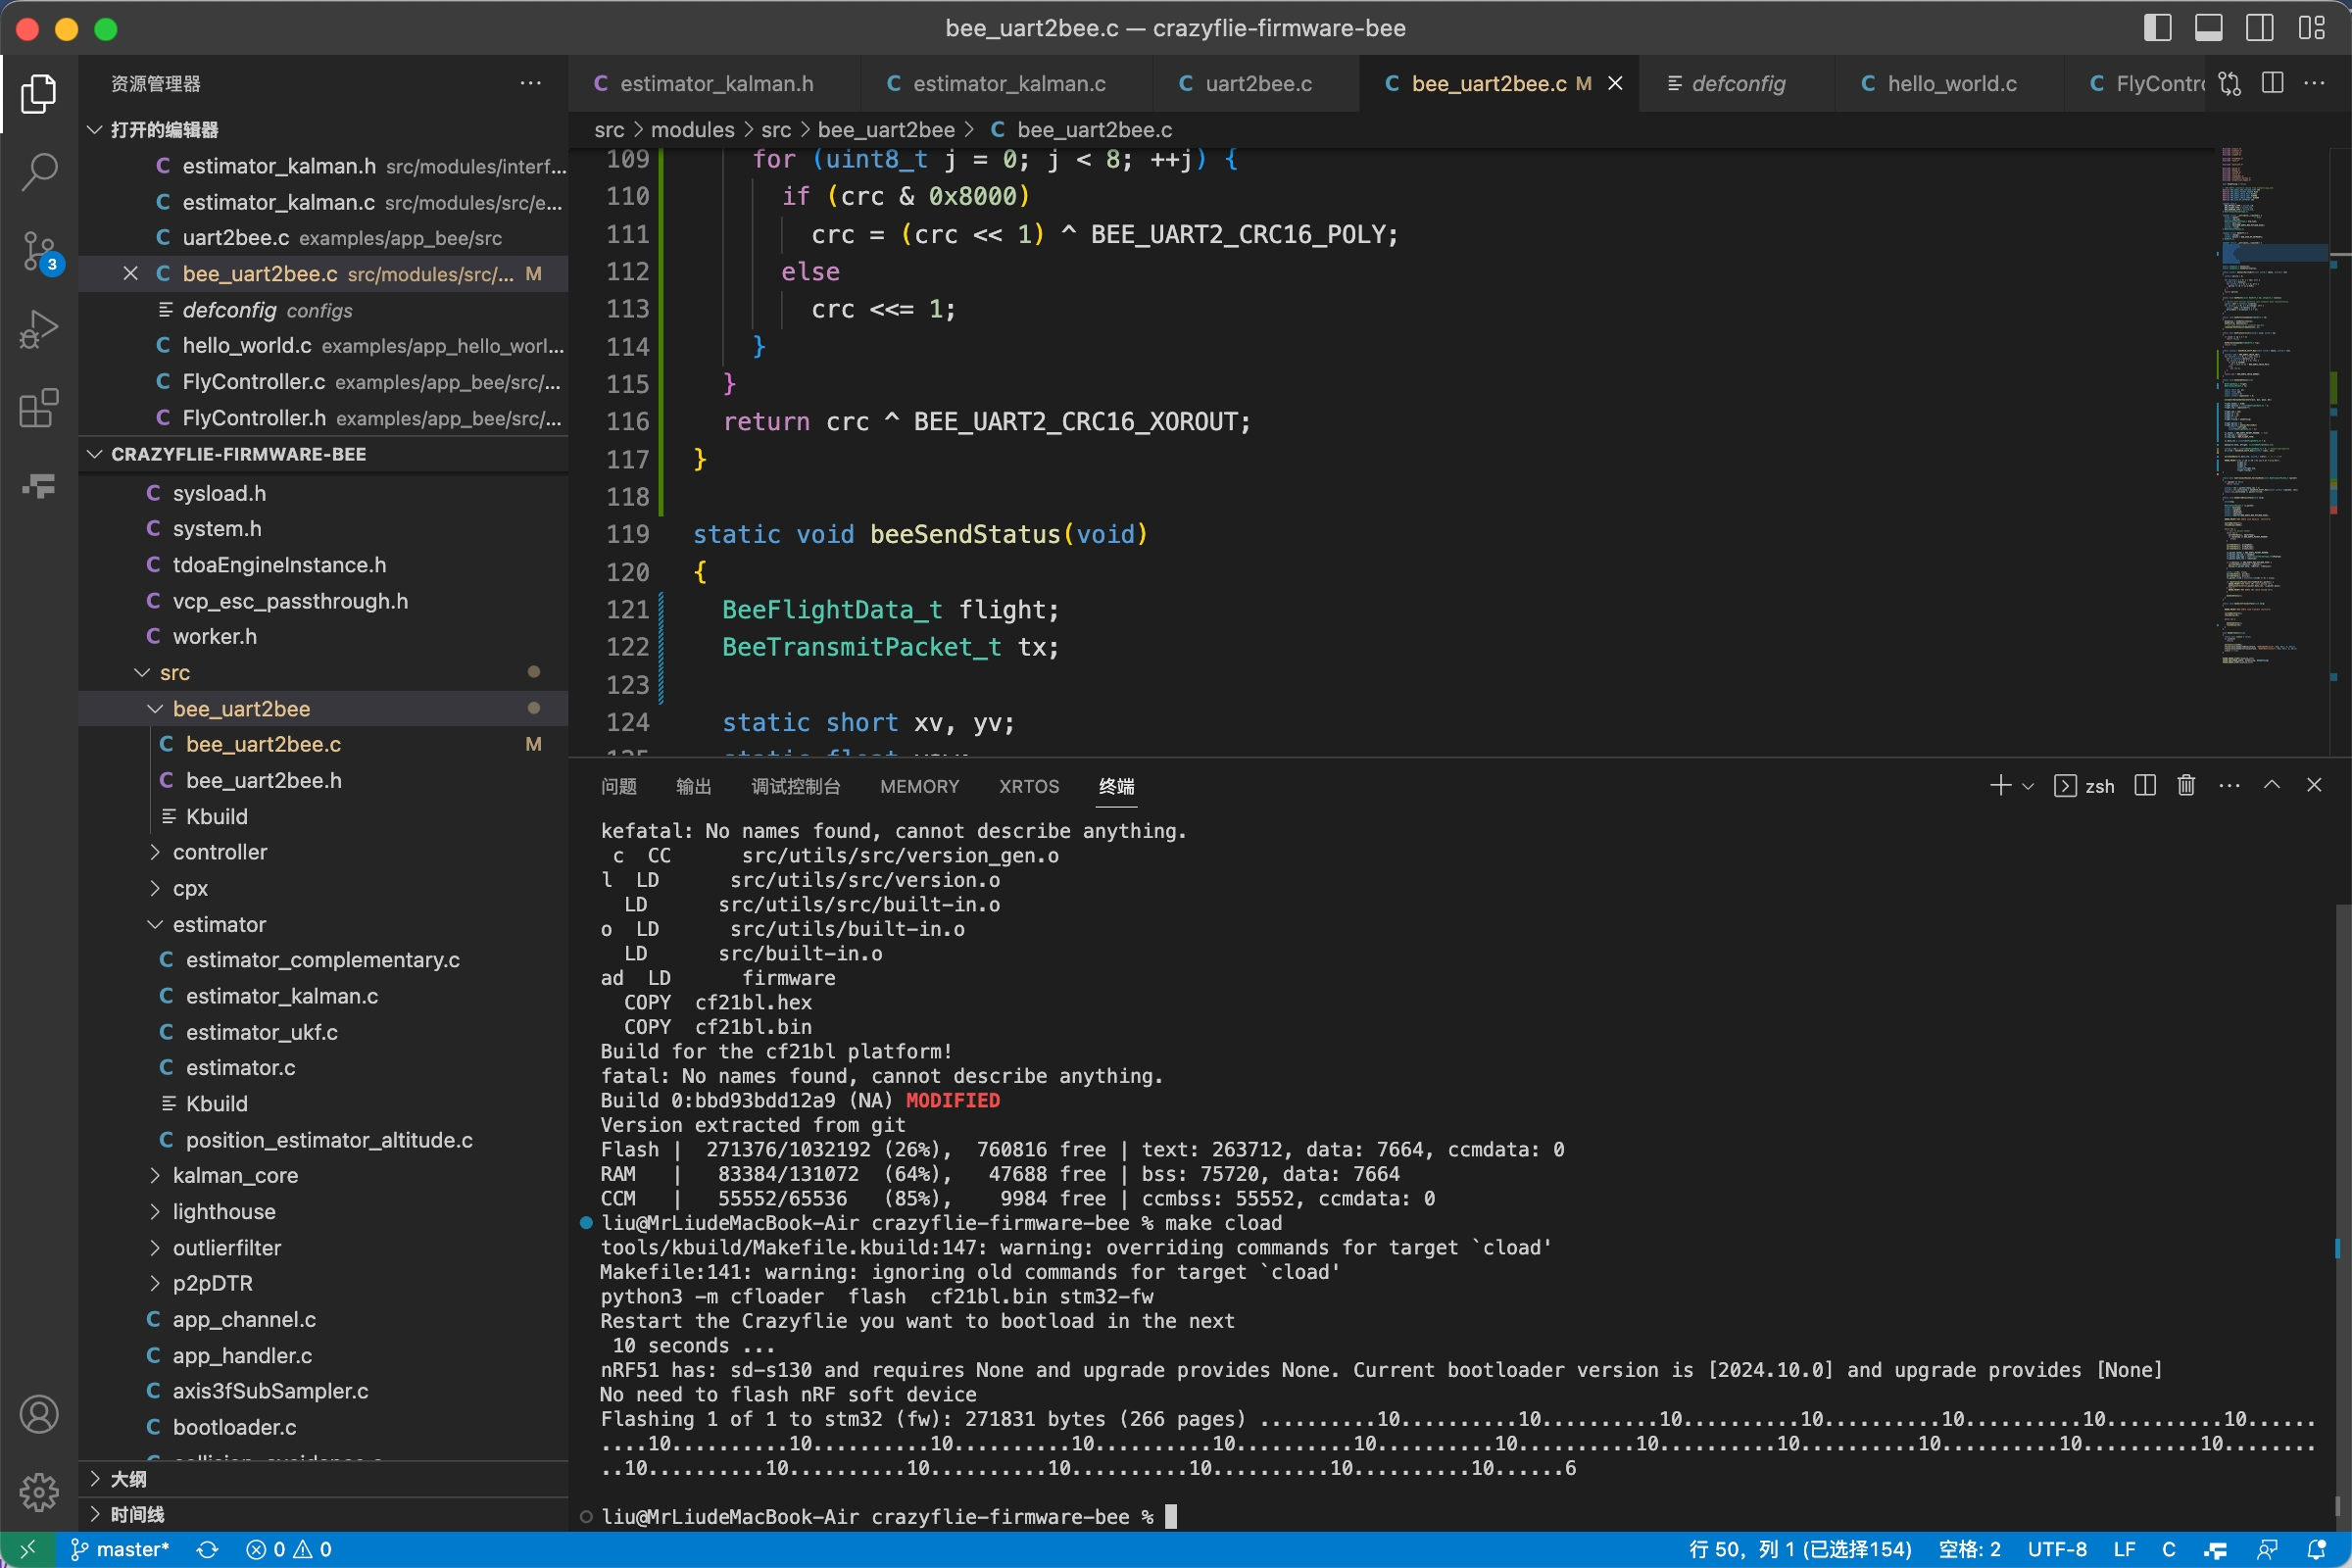
\includegraphics[width=.6\linewidth]{figures/content/chapter5/无人机编译烧录.jpg}
  \caption{无人机的编译与烧录}
  \label{fig:5_7}
\end{figure}

\begin{figure}[htbp]
  \centering
  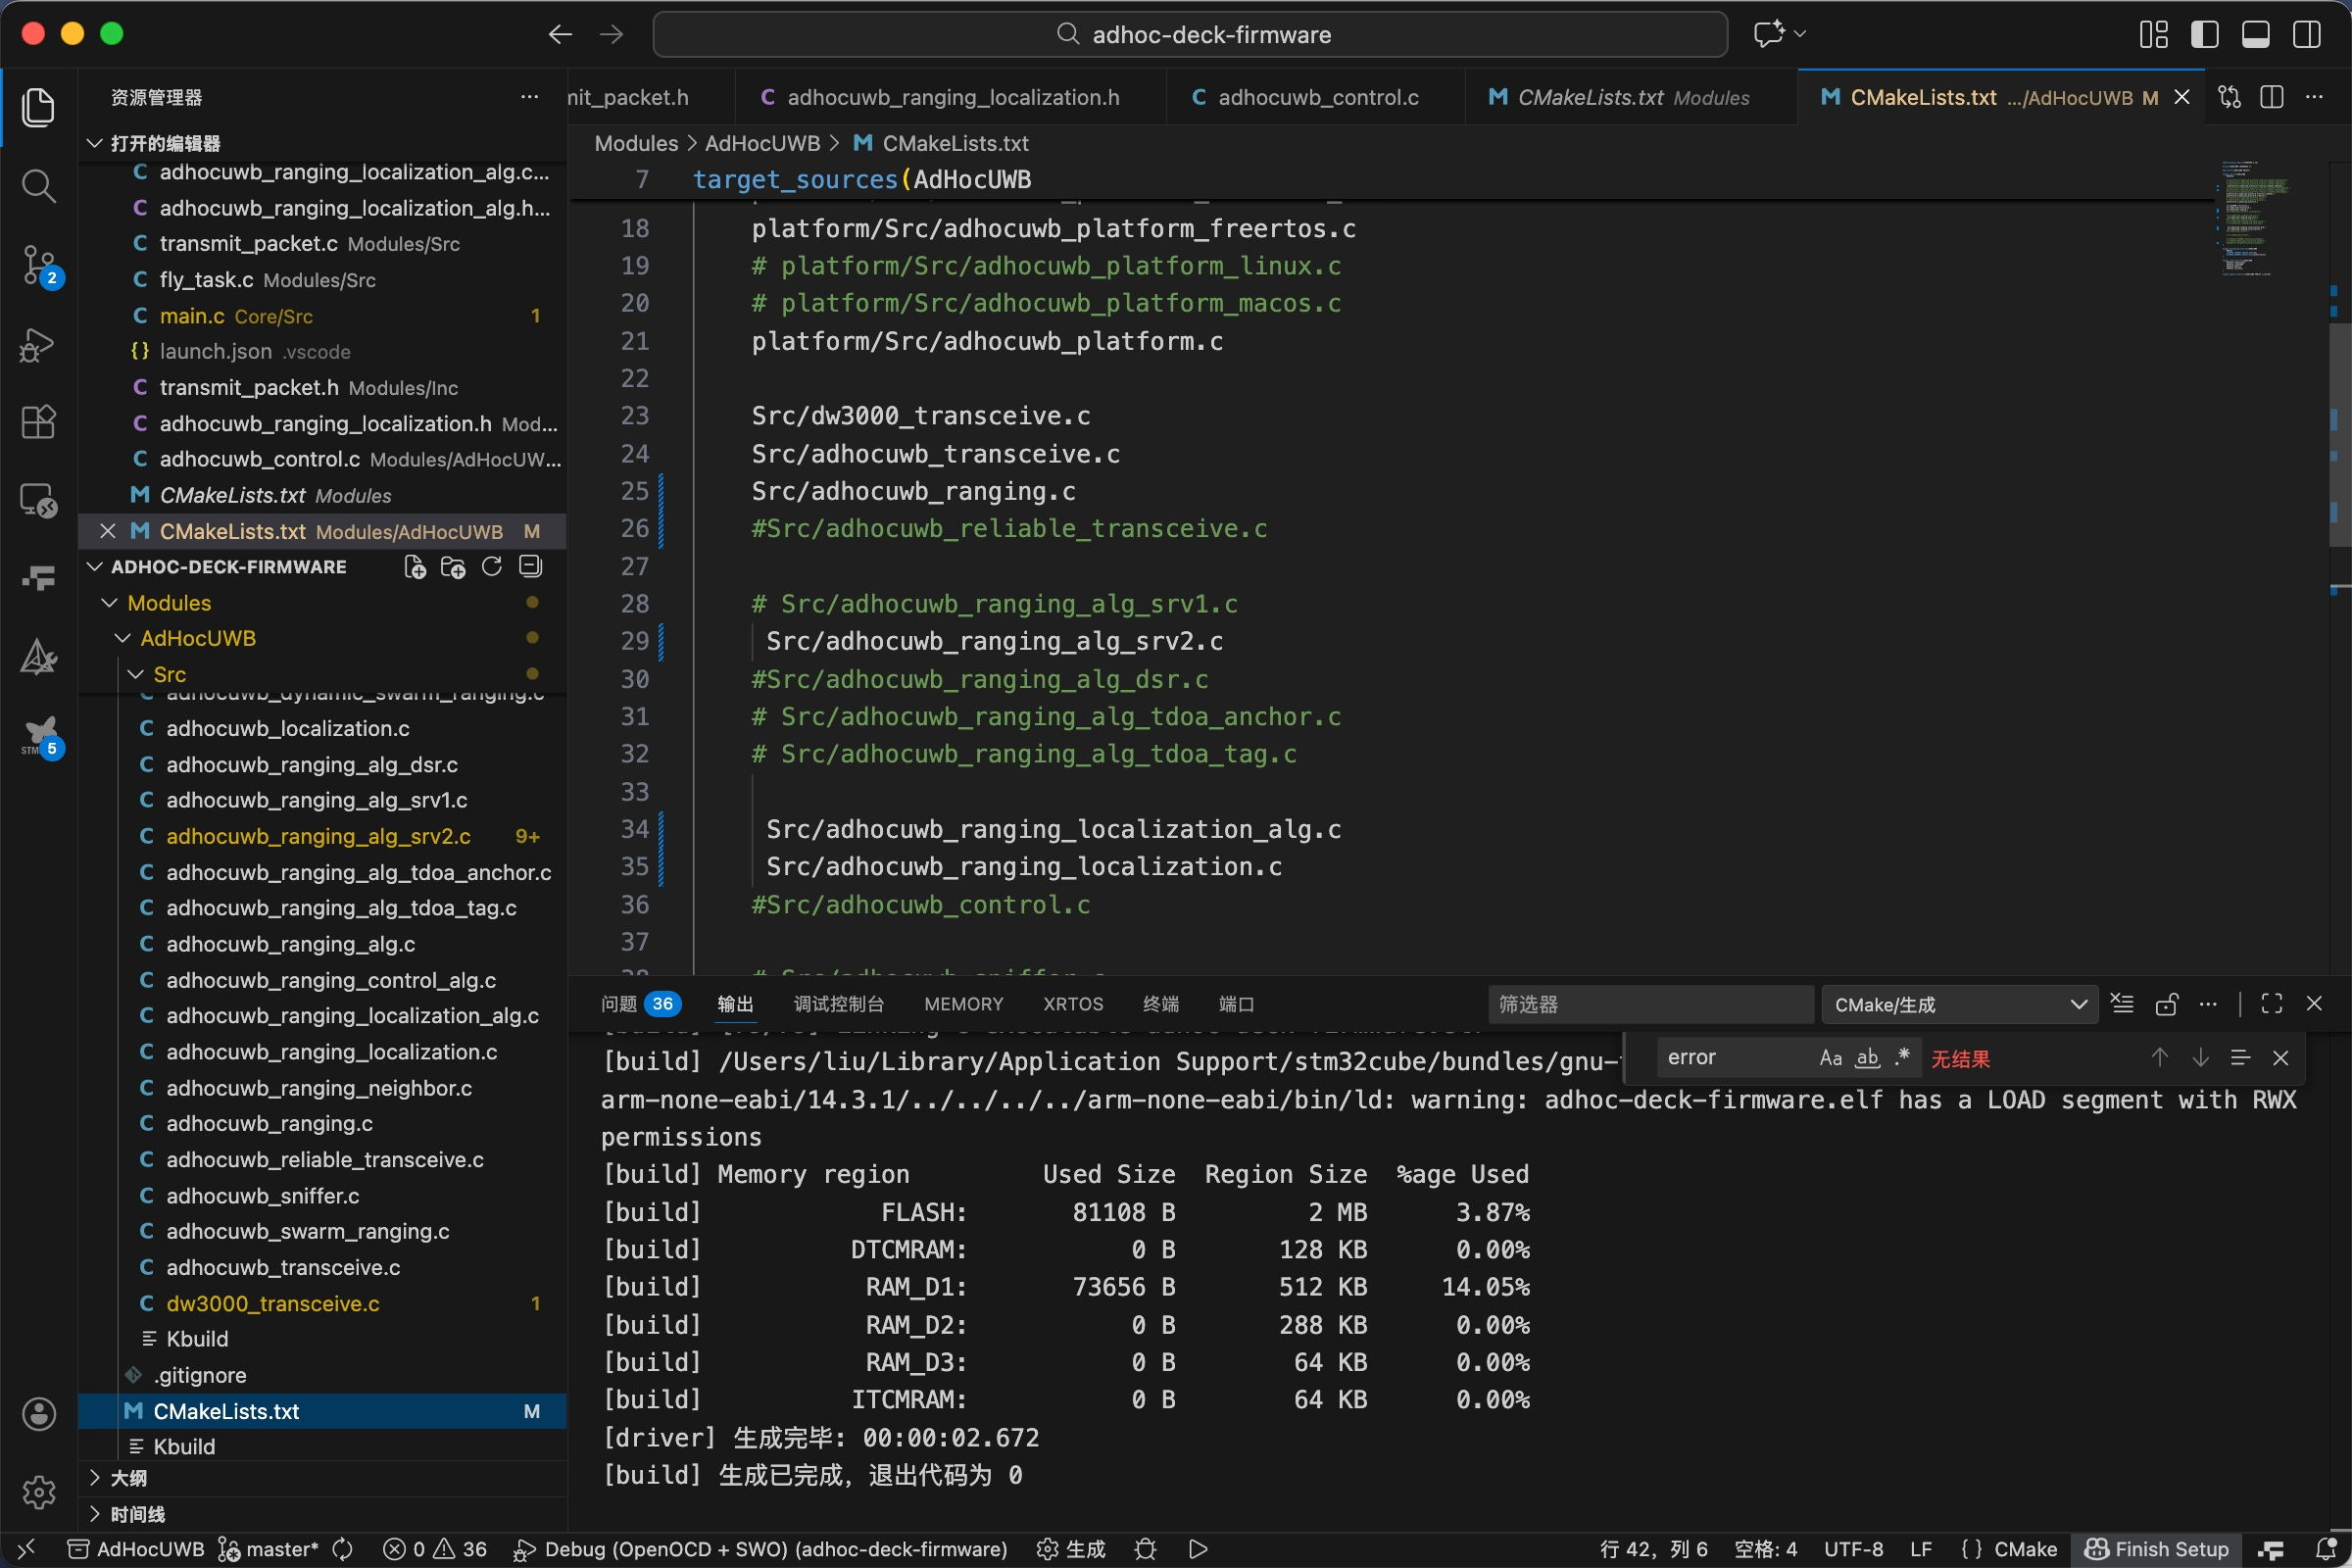
\includegraphics[width=.6\linewidth]{figures/content/chapter5/stmH7烧录.jpg}
  \caption{Adhoc Deck的编译与烧录}
  \label{fig:5_8}
\end{figure}

\begin{figure}[htbp]
  \centering
  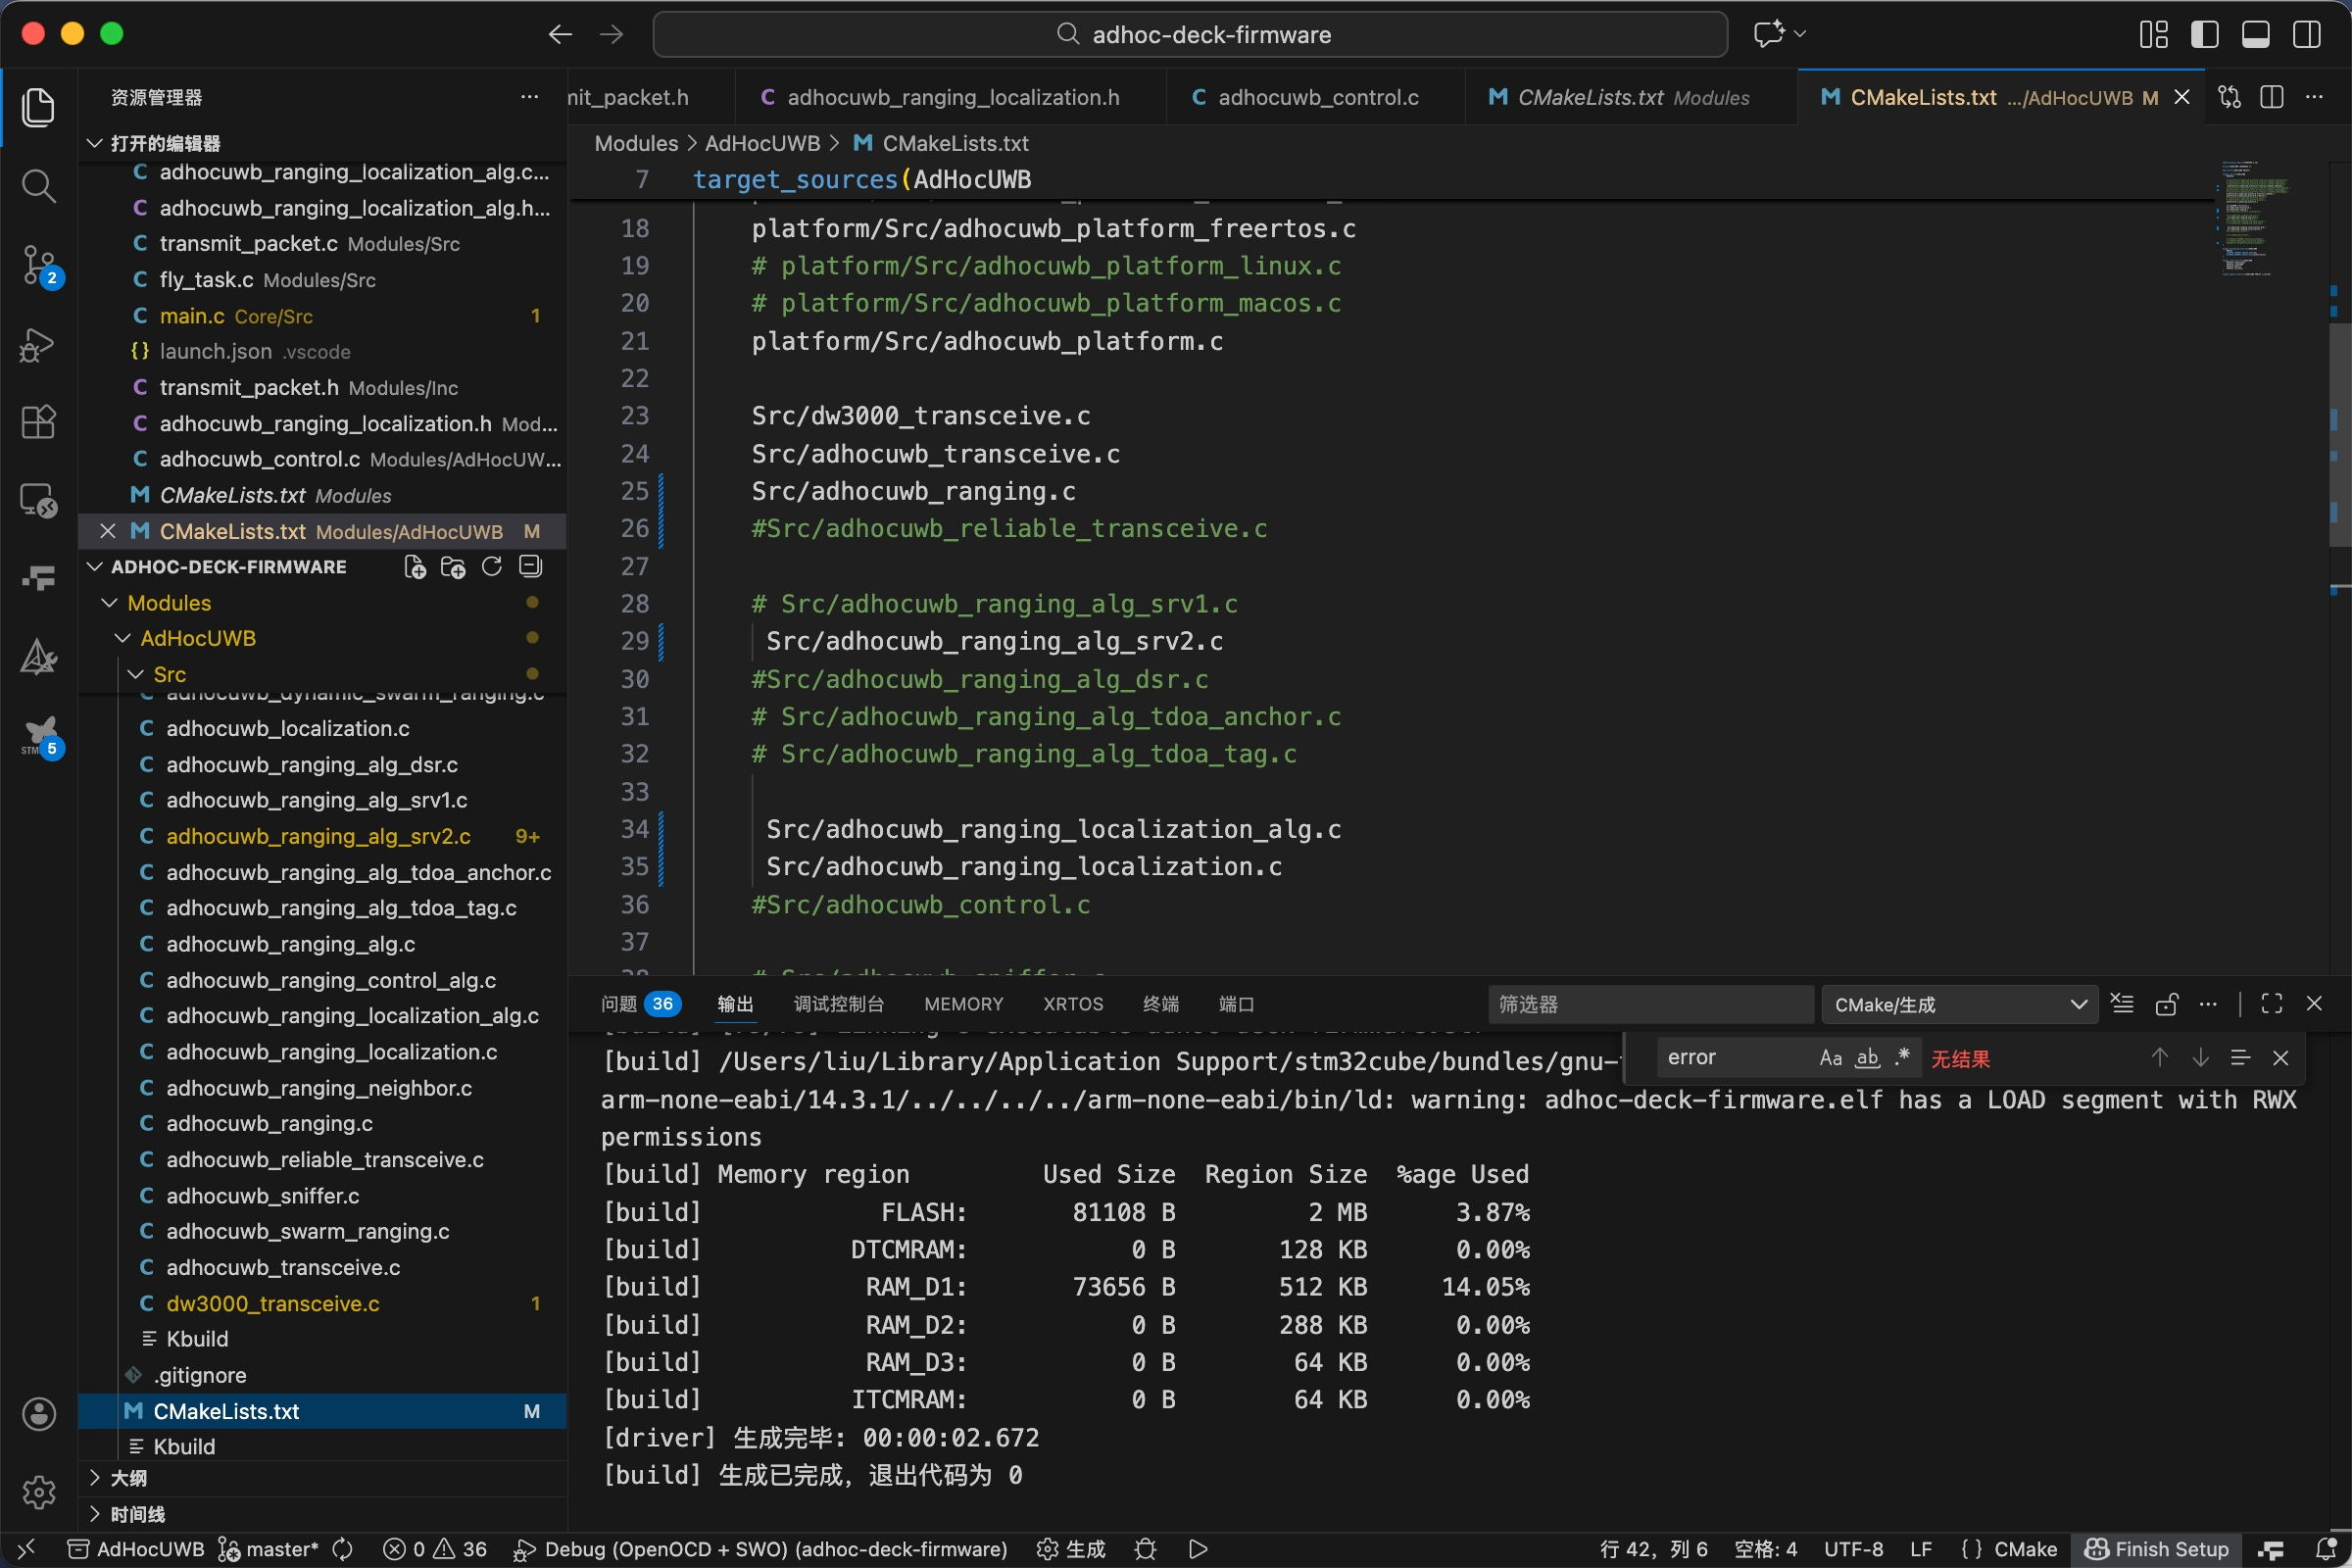
\includegraphics[width=.6\linewidth]{figures/content/chapter5/stmH7烧录.jpg}
  \caption{Adhoc Deck运行调试中的SWV输出}
  \label{fig:5_9}
\end{figure}
\section{ 系统测试与运行结果} 
%无人机编队飞行图以及Deck展示图

\section{本章小结} 

本章围绕微型无人机集群测距与自主导航原型系统的设计与实现，系统性地完成了从硬件构建到软件集成，再到实际飞行验证的整体工作，实现了前文算法研究向工程应用的有效落地。

在硬件方面，构建了由外部监控平台、领航无人机与跟随无人机组成的集群系统架构。通过集成 UWB 测距模块、光流与多方向距离传感器以及动捕系统，实现了多源信息融合的感知与定位能力，为集群协同提供了可靠的数据基础。
在软件方面，设计了分层模块化的软件架构，将系统划分为单机功能模块、集群协同模块以及算法支撑模块。针对领航与跟随两类无人机的不同功能需求，分别构建了自主导航、协同定位与局部避障等关键模块，并通过统一的数据流实现“感知—定位—决策—控制”的闭环运行机制。同时，结合 CRTP 通信协议与基于 UART 的高效数据传输机制，保障了系统在多节点协同下的实时性与稳定性。

在系统部署与实验验证方面，完成了无人机固件与嵌入式平台的编译烧录与调试，构建了真实飞行实验环境。实验结果表明，所设计的原型系统能够在资源受限的微型无人机平台上稳定运行，实现多无人机之间的可靠测距与协同定位，并支持领航—跟随模式下的自主导航与避障飞行，验证了本文所提方法在实际复杂环境中的可行性与有效性。


      % 第五章：
\chapter{总结与展望}


\section{论文总结}
本文围绕资源受限微型无人机在复杂未知环境中的协同感知与自主导航问题，针对集群测距、协同定位以及安全导航等关键技术展开了系统性研究，并完成了从算法设计到原型系统实现的完整验证。主要工作总结如下：

首先，针对微型无人机集群在高密度与高动态环境中测距不稳定的问题，本文在第三章提出了一种面向相对定位的鲁棒集群测距协议。通过对随机测距周期进行理论建模与参数优化，有效缓解了测距冲突与报文不匹配问题；同时引入不完全报文匹配下的补偿测距机制，提高了测距成功率。在此基础上，结合期望最大化算法，提出了一种自适应扩展卡尔曼滤波方法，实现了过程噪声与测量噪声的在线估计，从而在缺乏先验噪声信息的条件下提升了协同定位的精度与鲁棒性。

其次，针对无人机在复杂环境中自主导航面临的安全性不足问题，第四章提出了一种风险感知强化学习方法。该方法通过对回报分布进行建模，引入风险评估机制，使无人机在决策过程中能够兼顾收益与潜在风险，从而有效降低低概率高风险事件带来的影响。同时，通过对模型进行量化与压缩，实现了算法在资源受限嵌入式平台上的高效部署，满足了实时导航的需求。

最后，在第五章中，本文将所提出的协同定位方法与自主导航算法进行系统集成，构建了一个完整的微型无人机集群自主导航原型系统。该系统基于Crazyflie 2.1平台，采用“感知—定位—决策—控制”的分层架构，实现了多无人机之间的可靠测距、协同定位以及领航-跟随模式下的自主导航与避障。通过真实飞行实验验证，结果表明所构建系统能够在资源受限条件下稳定运行，具备良好的实时性与鲁棒性，验证了本文方法的工程可行性。

综上所述，本文从理论方法、算法设计到系统实现，系统性地解决了微型无人机集群在复杂环境中协同定位与安全导航的关键问题，为其在实际场景中的应用提供了重要参考。

\section{后续研究方向}
在前文工作的基础上，尽管本文已在微型无人机集群协同定位与自主导航方面取得了一定进展，但受限于研究条件与系统复杂性，相关方法在规模扩展、环境适应性以及协同智能水平等方面仍存在进一步提升空间。随着无人机技术与人工智能方法的不断发展，面向复杂动态环境的高效、安全与智能化集群系统将成为重要研究方向。基于此，本文结合第三章至第五章的研究内容，从协同测距与定位方法、风险感知决策机制以及系统集成与多机协同等方面，对未来可能的研究方向进行如下展望。
\subsection{集群测距与自适应定位方法的进一步研究（第三章）}
第三章主要解决了集群测距冲突与噪声未知条件下的协同定位问题，但仍存在一定的提升空间：

首先，在测距协议方面，本文采用随机周期与补偿机制来缓解冲突，但在更高密度集群或强干扰环境中，测距成功率仍可能下降。未来可研究基于时隙调度或自组织通信机制的测距协议，实现更加稳定和可预测的通信性能。同时，可结合图论方法，对测距拓扑结构进行优化，提高整体网络连通性。

其次，在测距误差建模方面，当前方法主要通过滤波进行补偿，缺乏对误差来源的精细建模。未来可针对非视距误差、多径效应等问题，引入环境感知或数据驱动的误差建模方法，从源头上提升测距精度。

再次，在自适应滤波方法方面，本文基于期望最大化算法实现了噪声协方差的在线估计，但其收敛速度和稳定性仍依赖一定条件。未来可研究更高阶自适应滤波方法（如UKF、IEKF或基于学习的滤波方法），并探索参数学习与状态估计的联合优化机制，以提升在强非线性场景下的性能。

最后，在分布式协同定位方面，当前方法仍存在一定集中处理特征。未来可进一步发展完全分布式定位算法，减少对单节点的依赖，提高系统的鲁棒性与可扩展性。

\subsection{风险感知强化学习导航方法的深化研究（第四章）}

第四章基于CVaR风险度量构建了风险感知强化学习导航方法，在提升无人机规避高风险行为方面取得了一定效果。然而，在复杂动态环境及工程落地过程中，仍存在进一步优化空间，具体体现在以下几个方面：

首先，在模型泛化能力方面，当前方法主要依赖于特定环境下的训练数据，其策略性能对环境分布具有一定依赖性。当环境发生变化（如障碍物分布、传感器噪声特性或动力学参数变化）时，策略可能出现性能退化甚至失效。为此，未来可引入域随机化（Domain Randomization）方法，通过在训练阶段对环境参数进行大范围扰动，使模型学习到更具鲁棒性的策略表示。此外，可结合迁移学习（Transfer Learning）或元学习（Meta-learning）方法，实现策略在不同任务或环境之间的快速适配，从而提升系统在未知场景中的泛化能力与实用性。

其次，在安全约束机制方面，尽管CVaR从风险分布角度对策略进行了约束，但其本质仍属于“软约束”，难以提供严格的安全保证。在实际无人机系统中，碰撞避免等安全约束往往具有“硬约束”特性。未来可考虑将强化学习与传统控制方法相结合，例如引入模型预测控制（Model Predictive Control, MPC）框架，在优化过程中显式加入状态与控制约束；或利用控制屏障函数（Control Barrier Function, CBF）构建安全过滤层，对强化学习输出的控制指令进行实时修正，从而形成“高层学习决策 + 低层安全约束”的分层控制结构，在保证安全性的同时兼顾策略的灵活性与最优性。

再次，在动态环境适应能力方面，当前方法主要针对静态或弱动态环境进行建模，对于快速变化的环境（如移动障碍物或多无人机交互场景）仍缺乏有效应对机制。未来可进一步研究时序建模方法（如引入循环神经网络RNN或注意力机制），增强策略对环境动态变化的感知能力；

此外，在轻量化与嵌入式部署方面，虽然本文已通过模型压缩降低了计算开销，但在更严格的资源受限平台（如纳型无人机）上仍存在实时性与功耗瓶颈。未来可从算法与硬件协同优化角度出发，进一步研究神经网络剪枝（Pruning）、知识蒸馏（Knowledge Distillation）以及量化感知训练（Quantization-Aware Training）等方法，在保证性能的前提下降低模型复杂度。同时，可探索基于专用加速硬件（如FPGA或边缘AI芯片）的部署方案，以实现高效、低功耗的实时推理。


\subsection{系统集成与多机协同能力提升（第五章）}

第五章完成了协同定位与风险感知导航方法的系统集成，构建了基于微型无人机平台的自主导航原型系统，并通过实验验证了系统的可行性与有效性。然而，从实际应用角度出发，系统在规模扩展、环境适应性以及协同智能水平等方面仍有进一步提升空间，未来可从以下几个方向展开研究：

首先，在系统规模扩展方面，当前系统主要面向小规模无人机集群进行设计与验证。当集群规模进一步扩大时，通信冲突、信息延迟及系统稳定性问题将更加突出。未来可研究面向大规模集群的分层式系统架构与通信调度机制，通过引入局部协同与全局协调相结合的策略，提高系统的可扩展性与运行效率。

其次，在复杂环境适应性方面，现有系统主要在室内或受控环境中进行验证，对于室外复杂环境（如动态障碍物、光照变化及弱定位条件）仍缺乏充分测试。未来可结合多传感器融合感知与环境建图技术，提升无人机在未知环境中的感知与定位能力，从而增强系统在真实场景中的适用性与鲁棒性。

再次，在多机协同决策能力方面，当前系统主要基于领航–跟随模式实现基础协同，其协同策略相对固定，难以适应复杂动态任务需求。未来可进一步引入多智能体强化学习（Multi-Agent Reinforcement Learning, MARL）方法，通过多无人机之间的协同学习与信息交互，实现去中心化的协同决策与自主任务分配。该方法能够使各无人机在局部观测条件下学习到协同避障与路径规划策略，从而在多障碍物、动态干扰及多机交互场景中显著提升系统整体性能与自适应能力。同时，可结合“集中训练–分布执行”机制，在保证实时性的前提下提高系统的可扩展性与稳定性。

最后，在软硬件协同优化方面，随着任务复杂度的提升，对计算资源与能耗提出了更高要求。未来可从系统层面出发，对计算、通信与控制模块进行联合优化，并结合嵌入式硬件加速技术，实现更高效、低功耗的无人机集群系统设计。      % 第六章：

%% ----------------------------------------------------------------------------
%%            Acknowledgement, Appendix, Bibliography and Resume
%% ----------------------------------------------------------------------------
//\input{chapters/acknowledgement}    % 致谢
\thesisbib{reference}               % 生成参考文献

%% 下面一句只是用于提示 TexPad 参考文献位置，正式生成时一定要删除
% \bibliography{reference.bib} % 告诉编译器参考文献所在文件

\input{chapters/appendix}           % 附录
% \input{chapters/resume}             % 作者简介

\end{document}
